\section{Reference figures}

% All the figures from Jim's web reports that have been used here

\subsection{From sections \ref{reverification} and \ref{finalCharacterization}}
\subsubsection{5x5 figures}

\subsubsection{Differential histograms}

% \subsubsection{Measurement histograms}
% \subsubsection{PTC curve}

\subsection{Web report reference figures}

A common tool for rapidly reviewing LSSTCam EO data are \href{https://s3df.slac.stanford.edu/data/rubin/lsstcam/}{web reports}, which provide full focal-plane, raft level, and sensor level figures of reference for prompt analysis of data runs. Web reports from runs 6 and 7 are available.

\subsubsection{Focal-plane level}
% \paragraph{Focal-plane layout}

\paragraph{Focal-plane mosaics for different quantities}

Focal plane mosaics consist of fully assembled focal planes, with amplifiers colored according to the associated measurement. The full focal-plane mosaics are generated for most eo-pipe parameters and are scaled appropriately for each parameter. These plots provide a visualization that shows differences in e2v and ITL sensors across the focal plane, and the uniformity.

\begin{figure}[h]
    \centering
    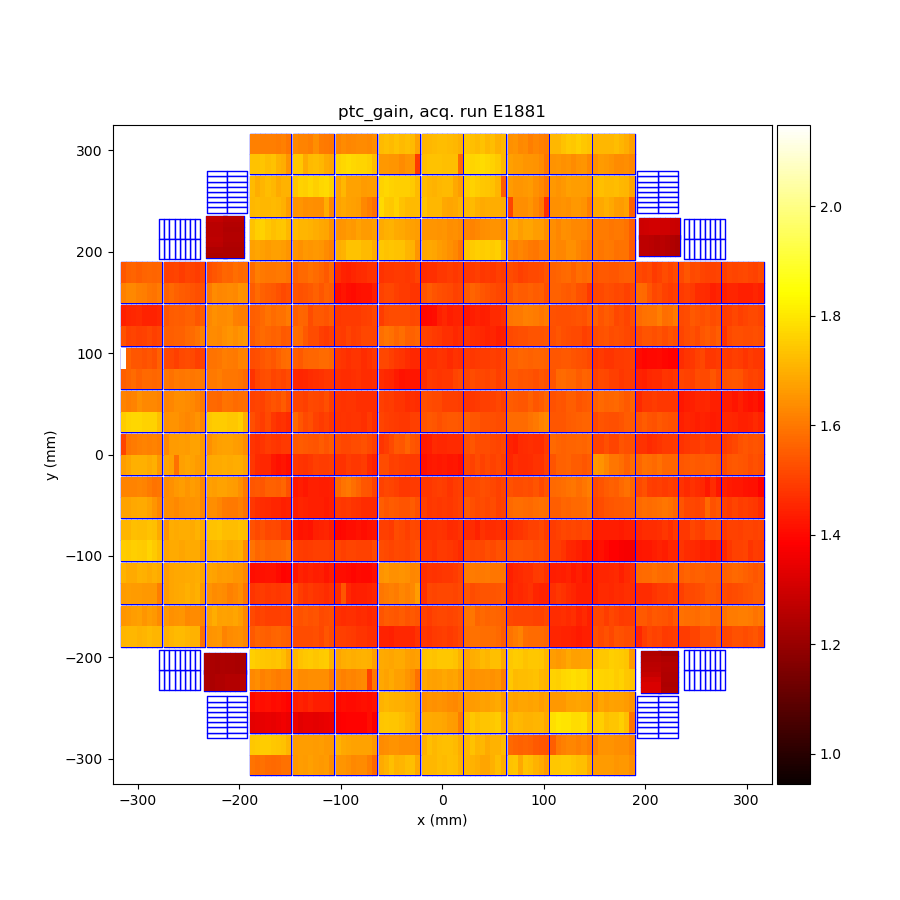
\includegraphics[width=0.8\linewidth]{figures/ReferenceFigures/ptc_gain_plot_LSSTCam_u_lsstccs_eo_ptc_plots_E1881_w_2024_35_20241105T131208Z.png}
    \caption{A focal plane mosaic from run E1881 for PTC gain}
    \label{fig:ref:fpMosaic}
\end{figure}

\paragraph{Histograms}

In addition to focal-plane mosaics, histograms are created for all eo-pipe metrics. These histograms have bins and ranges specific to each parameter. For some parameters, the histograms provide a neat visualization to quantify differences in e2v and ITL measurements, such as figure \ref{fig:ref:histogram} for PTC $a_{00}$. 

\begin{figure}[h]
    \centering
    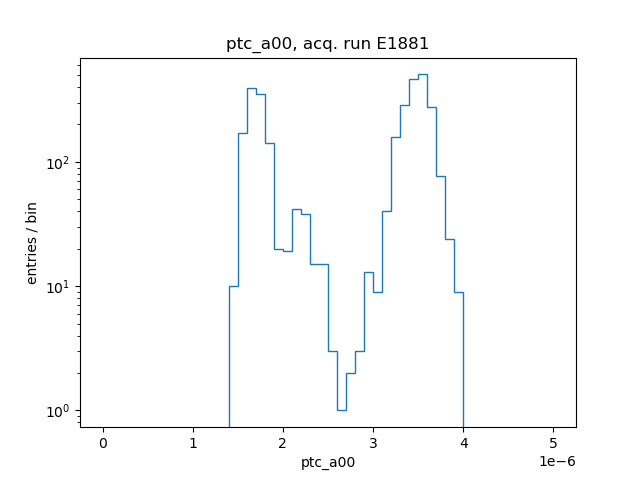
\includegraphics[width=0.8\linewidth]{figures/ReferenceFigures/ptc_a00_hist_LSSTCam_u_lsstccs_eo_ptc_plots_E1881_w_2024_35_20241105T131208Z.png}
    \caption{A histogram from run E1881 for PTC $a_{00}$}
    \label{fig:ref:histogram}
\end{figure}

\subsubsection{Raft level}

\paragraph{Correlation figures}

Correlation figures are created on the raft level for all science rafts. Two types of correlation figures are created; one for the imaging region, and one for the overscan region. The correlation computed is a Pearson correlation coefficient.

\begin{figure}[h]
    \centering
    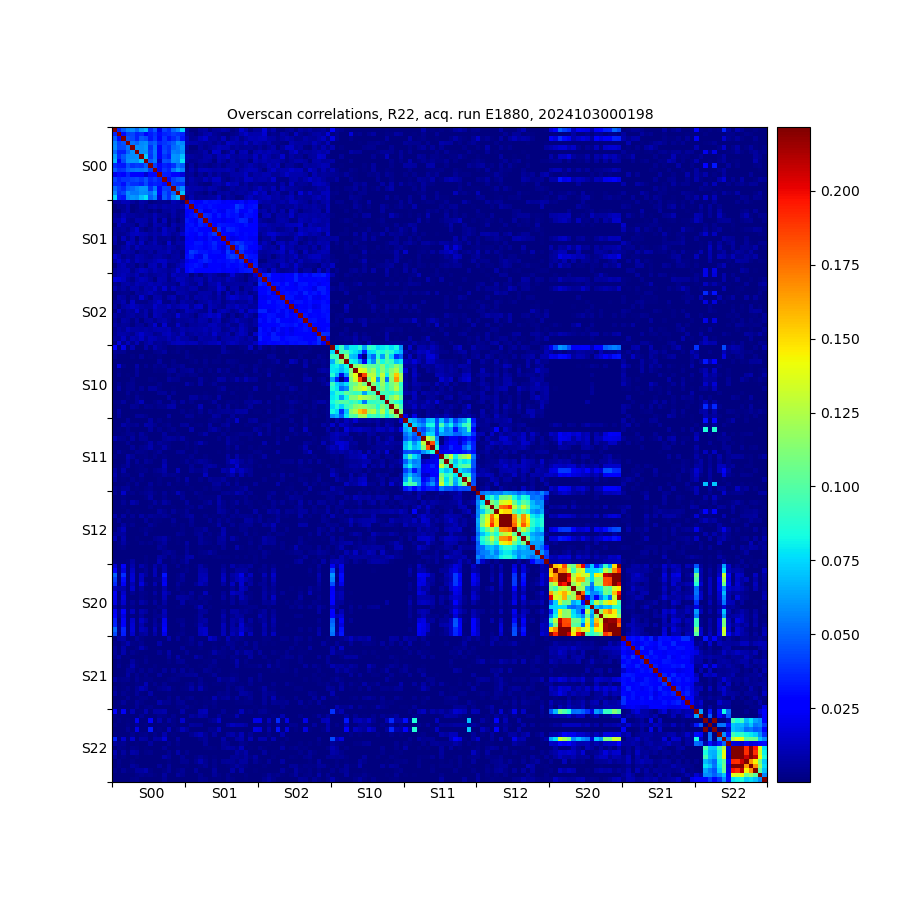
\includegraphics[width=0.8\linewidth]{figures/ReferenceFigures/overscan_correlation_plot_LSSTCam_R22_S00_u_lsstccs_eo_raft_amp_correlations_E1880_w_2024_35_20241101T015955Z.png}
    \caption{Overscan correlations for R22\_S11 in run E1880.}
    \label{fig:ref:overscanCorrelations}
\end{figure}

\paragraph{Lambda mosaics}

As a part of the standard B protocol, flats are taken in different LEDs to provide a chromatic response across the bandpass relevant to LSST. The mosaic is assembled on the raft level, and short wavelength flats show the laser annealing pattern characteristic to e2v sensors (see figure \ref{fig:ref:blueLambda}).

\begin{figure}[h]
    \centering
    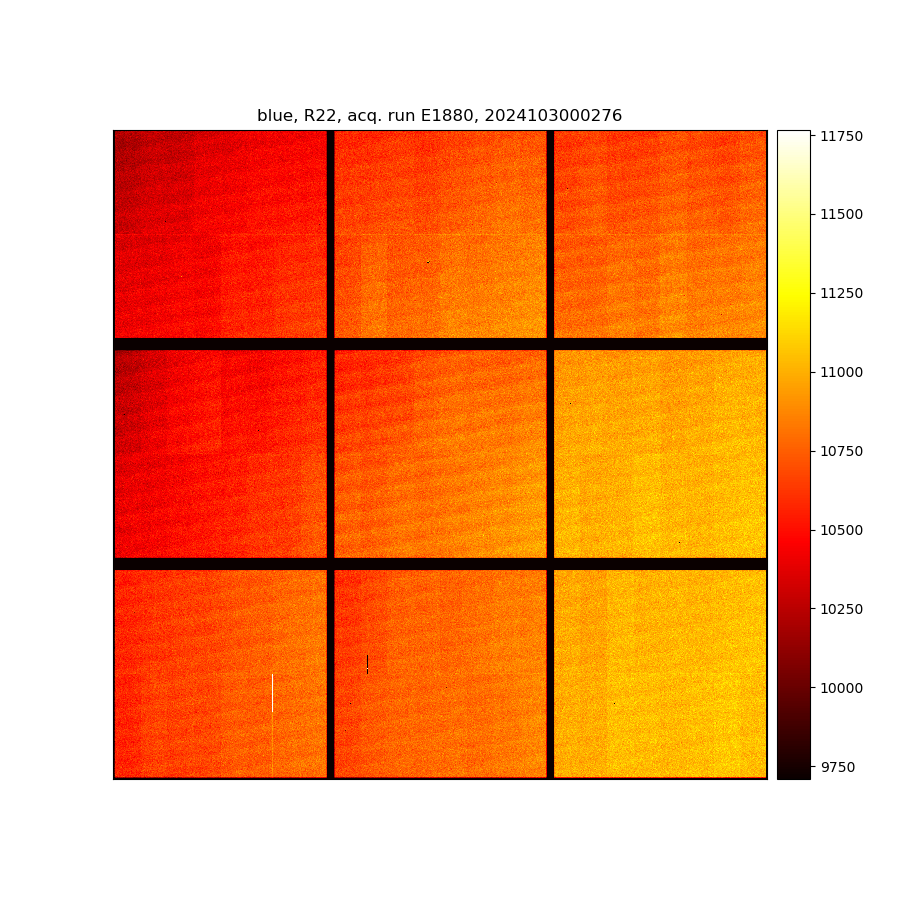
\includegraphics[width=0.8\linewidth]{figures/ReferenceFigures/eoRaftMosaic_LSSTCam_blue_MC_C_20241030_000276_R22_S00_u_lsstccs_eo_raft_lambda_mosaics_E1880_w_2024_35_20241101T020341Z.png}
    \caption{Blue led mosaic for R22 from run E1880.}
    \label{fig:ref:blueLambda}
\end{figure}

\paragraph{Calibration frames}

For runs with bias dark and flat frames (most commonly B protocols), combined calibrations are produced and assembled on the raft level. These mosaics are gain corrected.

\begin{figure}[h]
    \centering
    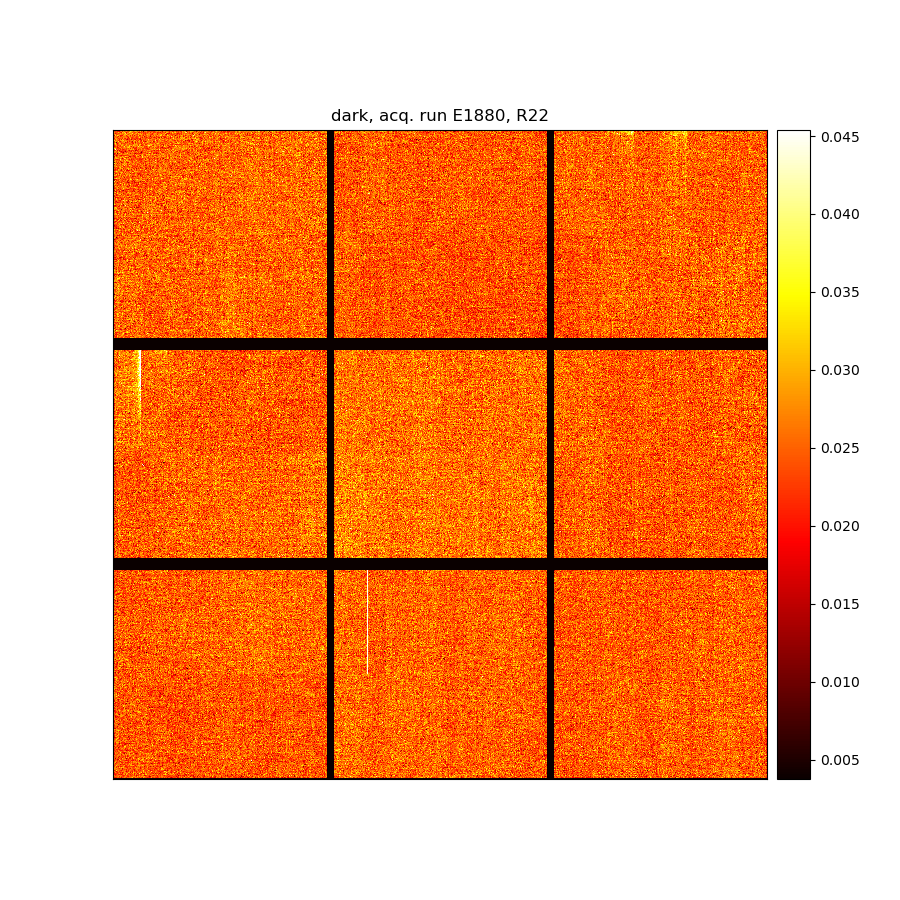
\includegraphics[width=0.8\linewidth]{figures/ReferenceFigures/eoDarkRaftMosaic_LSSTCam_R22_S00_u_lsstccs_eo_raft_calib_mosaics_E1880_w_2024_35_20241101T020324Z.png}
    \caption{Calibration dark for R22 from run E1880, extracted using B protocol dark sequence.}
    \label{fig:ref:calibFrame}
\end{figure}

\paragraph{Bias stability}

Bias stability figures are created for acquisition sequences that acquire multiple bias frames. Three different bias stability plots are created; amp-wise mean vs time, amp-wise standard deviation vs time, amp-wise mean vs time for region covering the readout corner.

\begin{figure}[h]
    \centering
    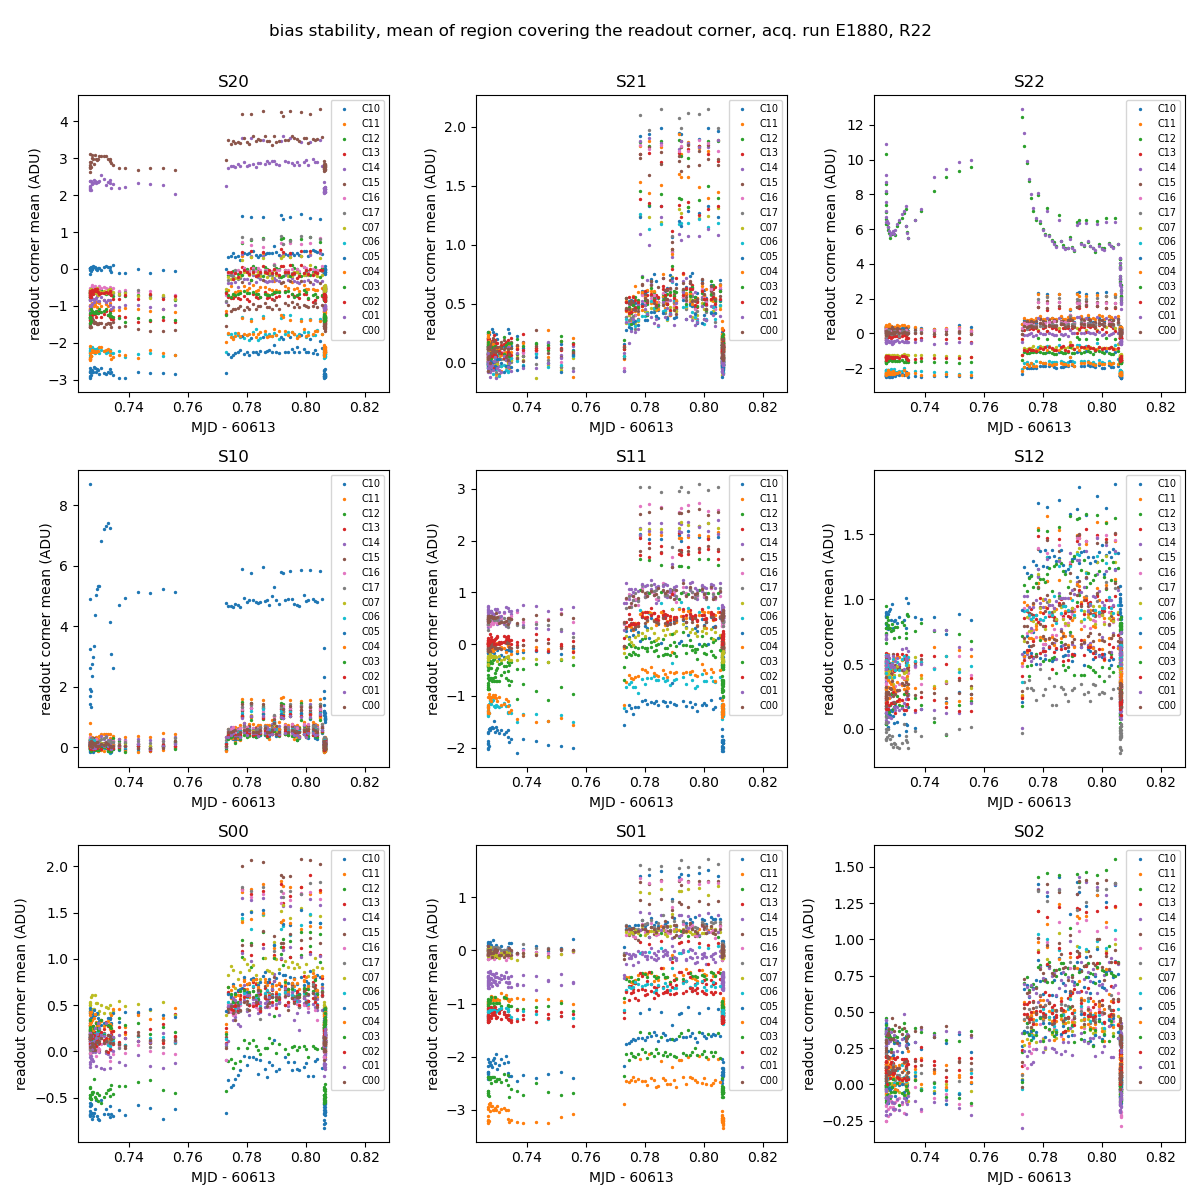
\includegraphics[width=0.8\linewidth]{figures/ReferenceFigures/bias_rc_mean_vs_time_plot_LSSTCam_R22_S00_u_lsstccs_eo_bias_stability_E1880_w_2024_35_20241101T020021Z.png}
    \caption{Bias stability mean vs time in readout corner for R22 from run E1880.}
    \label{fig:ref:biasStability}
\end{figure}

\paragraph{Divisadero profiles}

Divisadero tearing profiles are created for each raft, with divisadero response grouped along the mid-line break. The regions of individual amplifiers are marked by dashed lines to show regions where divisadero response is expected.

\begin{figure}
    \centering
    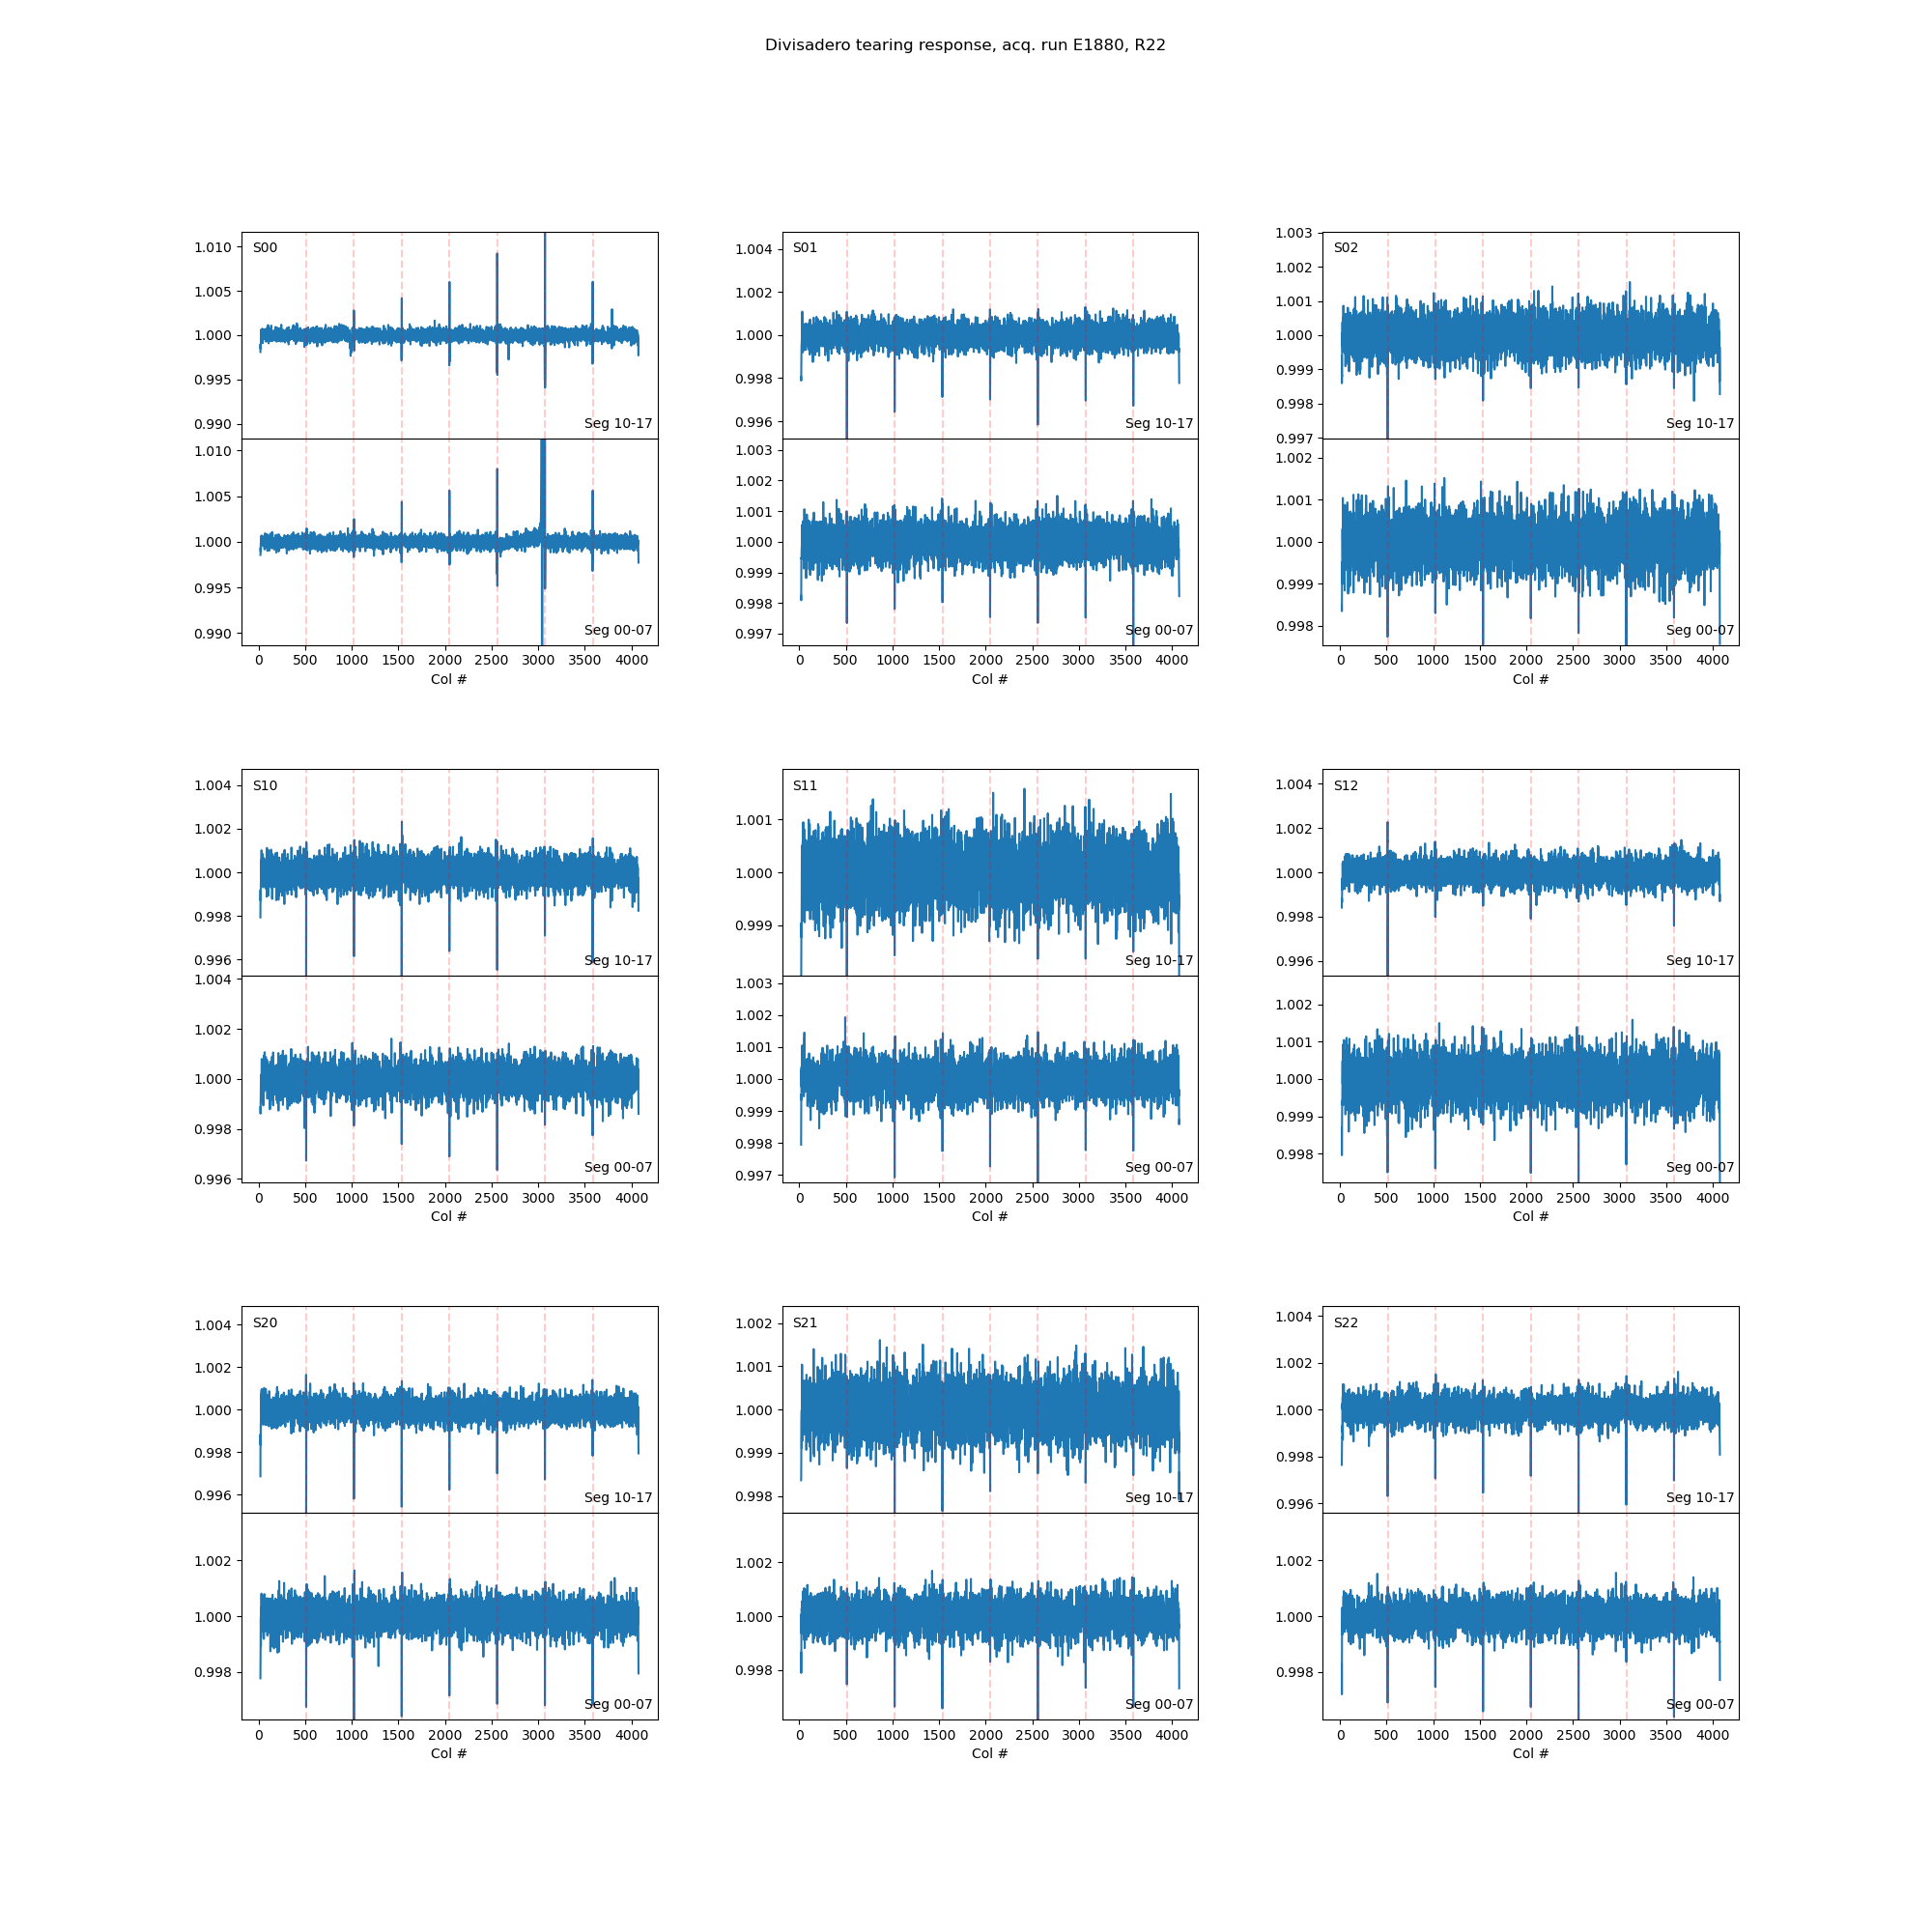
\includegraphics[width=0.8\linewidth]{figures/ReferenceFigures/divisadero_raft_plot_LSSTCam_R22_S00_u_lsstccs_eo_divisadero_tearing_E1880_w_2024_35_20241101T020421Z.png}
    \caption{Divisadero tearing profile for R22 from run E1880.}
    \label{fig:ref:divisaderoProfile}
\end{figure}

\subsubsection{Sensor level}

\paragraph{Bias profiles}

Bias profiles are created for each sensor, along both serial and parallel directions. Amplifiers are plotted separately to allow for amplifier dependent response to be identified. Different columns/rows are plotted in different colors to allow for identification of problematic columns/rows.

\begin{figure}
    \centering
    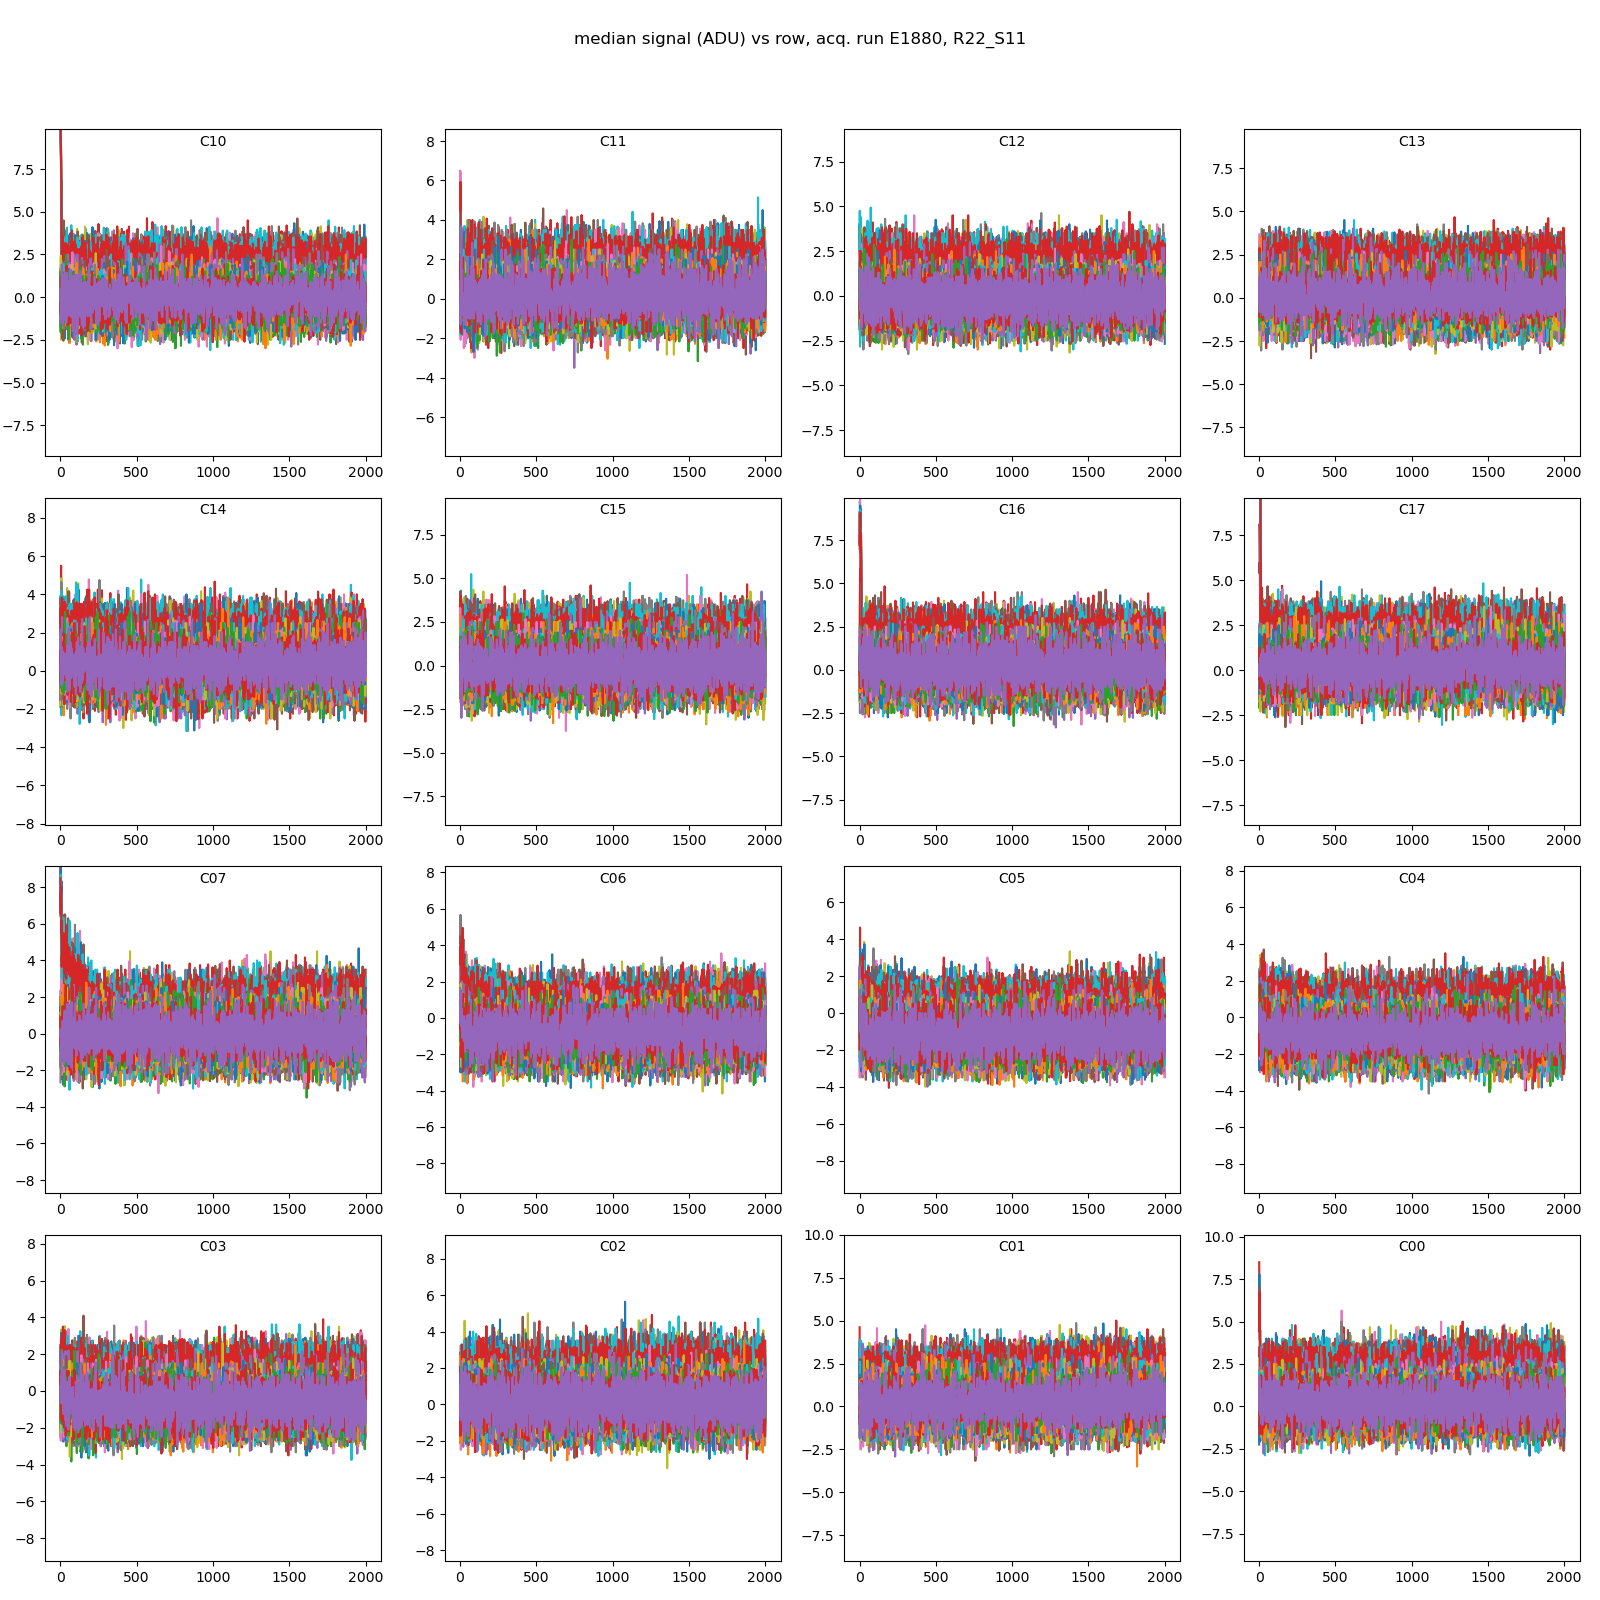
\includegraphics[width=0.8\linewidth]{figures/ReferenceFigures/bias_parallel_profile_plots_LSSTCam_R22_S11_u_lsstccs_eo_bias_stability_E1880_w_2024_35_20241101T020021Z.png}
    \caption{Median bias profile in the parallel direction for R22\_S11 from run E1880.}
    \label{fig:ref:biasProfile}
\end{figure}

\paragraph{PTCs}

PTC plots are created for each sensor, and separated by amplifier. For each amplifier, a PTC curve is created. PTC gain, $a_{00}$, and turnoff (in ADU) is shown for each amplifier.

\begin{figure}
    \centering
    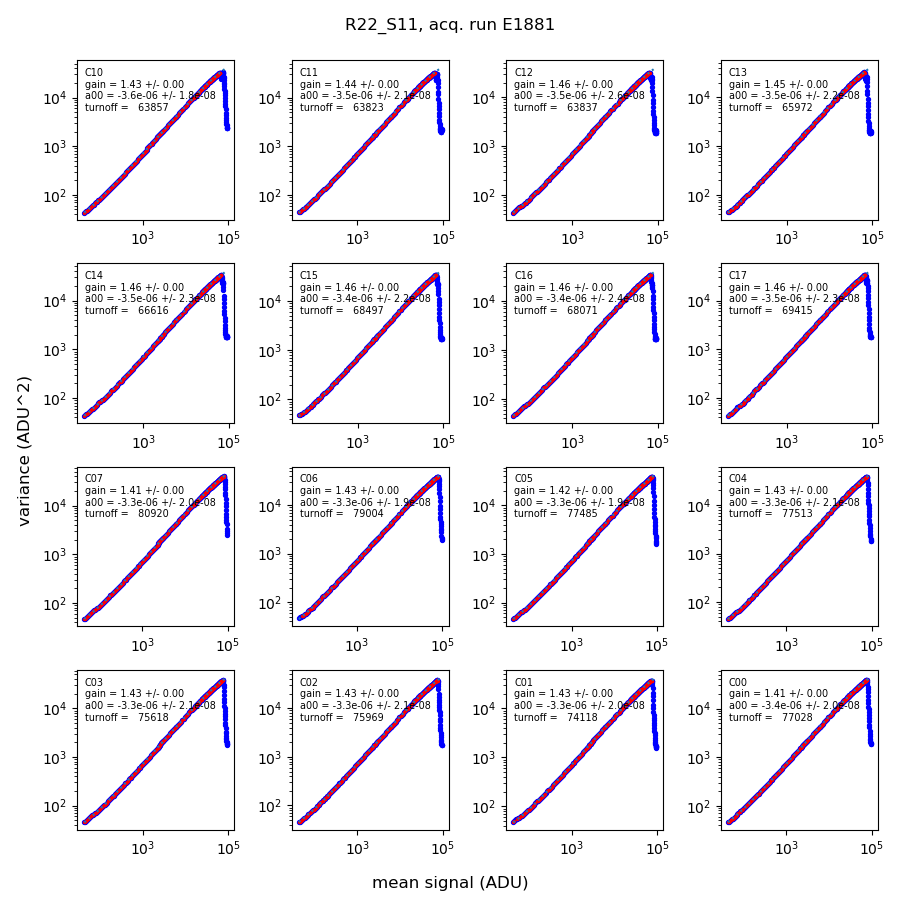
\includegraphics[width=0.8\linewidth]{figures/ReferenceFigures/ptc_plots_LSSTCam_R22_S11_u_lsstccs_eo_ptc_plots_E1881_w_2024_35_20241105T131208Z.png}
    \caption{PTC plots for R22\_S11 from run E1881.}
    \label{fig:ref:PTCs}
\end{figure}

\paragraph{Nonlinearity}

\paragraph{Data from flat pairs}

\paragraph{CTI}

\paragraph{BF covariances}

\paragraph{Persistence figure}


\clearpage

\section{OCS integration}

\clearpage
\section{Phosphorescence}\label{appendix:phosphorescence}
\clearpage
\section{Phosphorescence identification on ITL set of sensors}

\begin{figure}[!htbp]
\centering
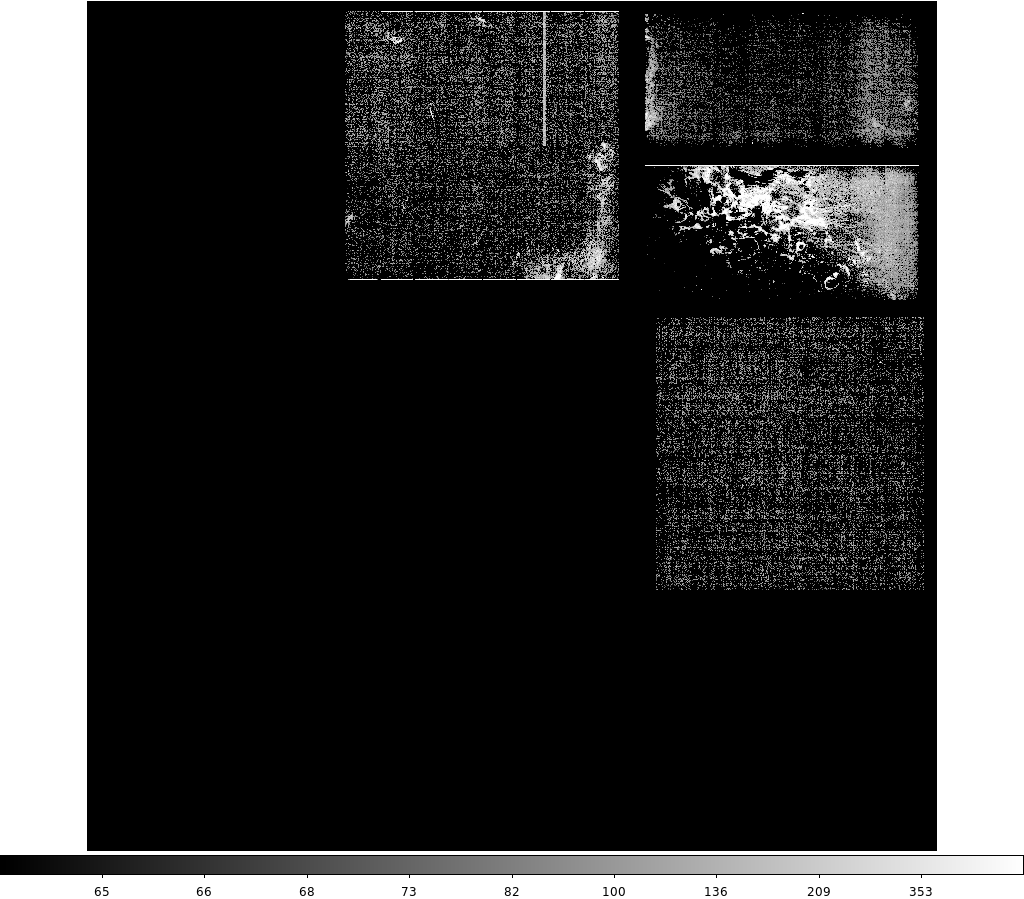
\includegraphics[width=0.9\textwidth]{figures/phosphorescence-survey/itl_fluor_R00_0-19_rb1_log.png}
\caption{Phosphorescence transients for the R00 CRTM captured in the first 15\,s following {\it red} CCOB LED at 400\,ke$^-$/pix. With 8$\times$8 blocking, the upper end of the color scale (640) corresponds to 10\,e$^-$/pixel when averaged over 64 pixels contributing.}
\label{fig:phos:R00}
\end{figure}

\begin{figure}[!htbp]
\centering
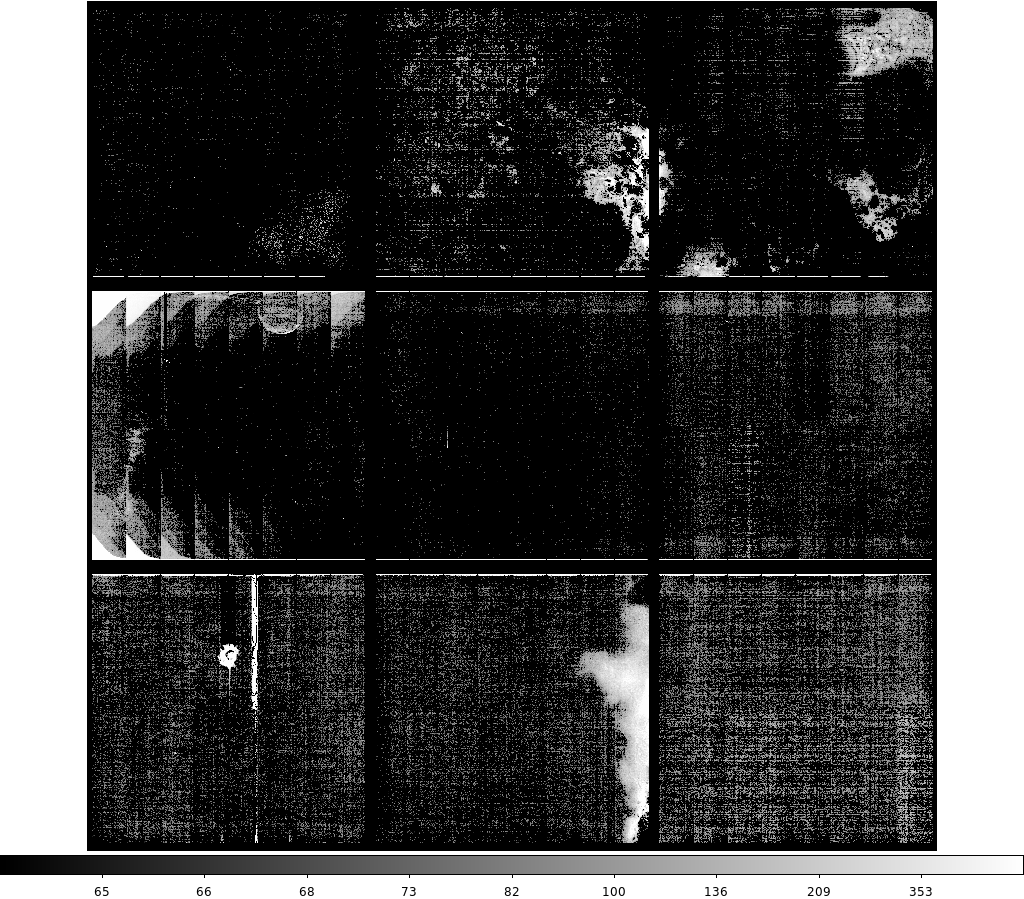
\includegraphics[width=0.9\textwidth]{figures/phosphorescence-survey/itl_fluor_R01_0-19_rb1_log.png}
\caption{Phosphorescence transients for the R01 RTM captured in the first 15\,s following {\it red} CCOB LED at 400\,ke$^-$/pix. With 8$\times$8 blocking, the upper end of the color scale (640) corresponds to 10 e$^-$/pixel when averaged over 64 pixels contributing.}
\label{fig:phos:R01}
\end{figure}

\begin{figure}[!htbp]
\centering
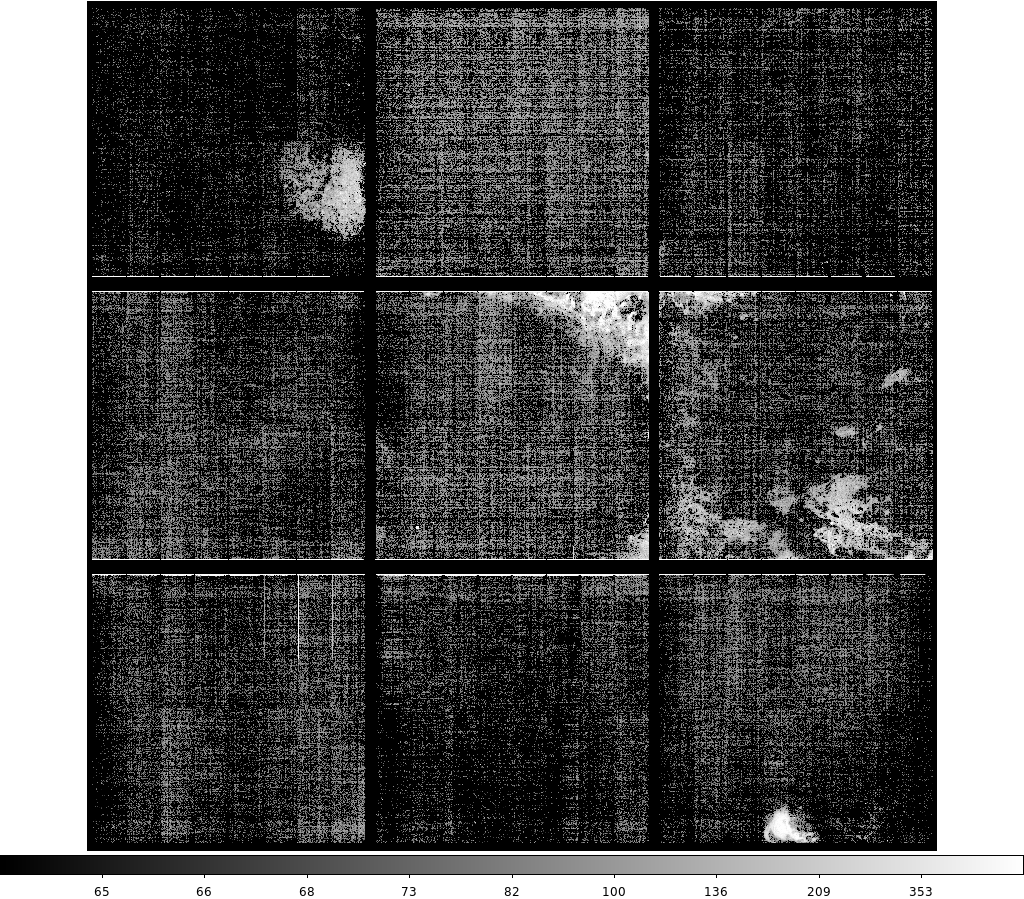
\includegraphics[width=0.9\textwidth]{figures/phosphorescence-survey/itl_fluor_R02_0-19_rb1_log.png}
\caption{Phosphorescence transients for the R02 RTM captured in the first 15\,s following {\it red} CCOB LED at 400\,ke$^-$/pix. With 8$\times$8 blocking, the upper end of the color scale (640) corresponds to 10 e$^-$/pixel when averaged over 64 pixels contributing.}
\label{fig:phos:R02}
\end{figure}

\begin{figure}[!htbp]
\centering
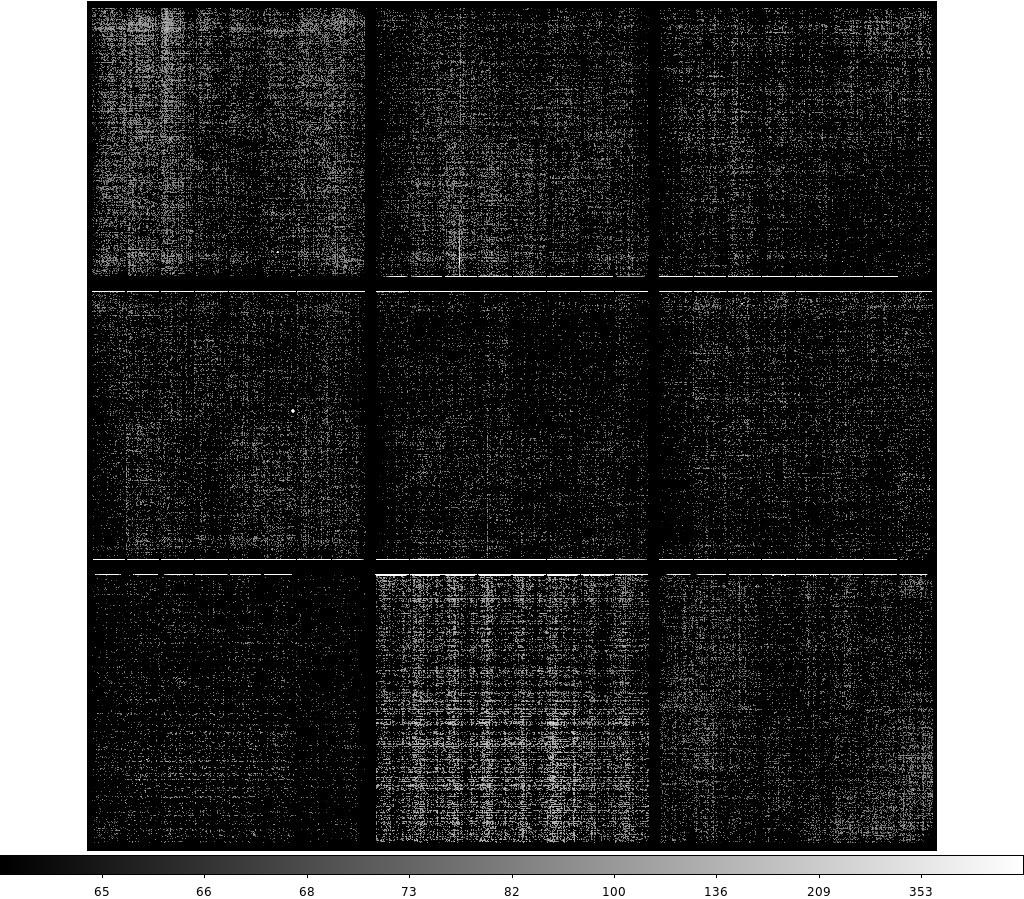
\includegraphics[width=0.9\textwidth]{figures/phosphorescence-survey/itl_fluor_R03_0-19_rb1_log.png}
\caption{Phosphorescence transients for the R03 RTM captured in the first 15\,s following {\it red} CCOB LED at 400\,ke$^-$/pix. With 8$\times$8 blocking, the upper end of the color scale (640) corresponds to 10 e$^-$/pixel when averaged over 64 pixels contributing.}
\label{fig:phos:R03}
\end{figure}

\begin{figure}[!htbp]
\centering
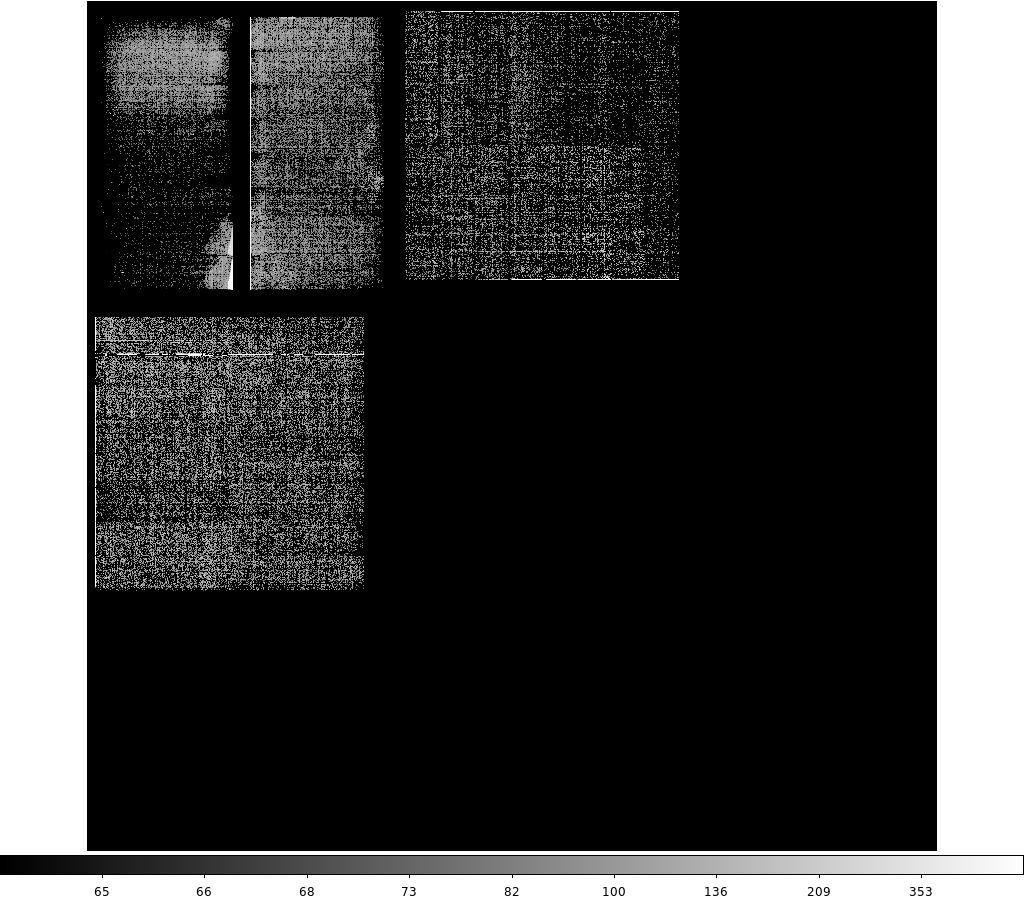
\includegraphics[width=0.9\textwidth]{figures/phosphorescence-survey/itl_fluor_R04_0-19_rb1_log.png}
\caption{Phosphorescence transients for the R04 CRTM captured in the first 15\,s following {\it red} CCOB LED at 400\,ke$^-$/pix. With 8$\times$8 blocking, the upper end of the color scale (640) corresponds to 10 e$^-$/pixel when averaged over 64 pixels contributing.}
\label{fig:phos:R04}
\end{figure}

\begin{figure}[!htbp]
\centering
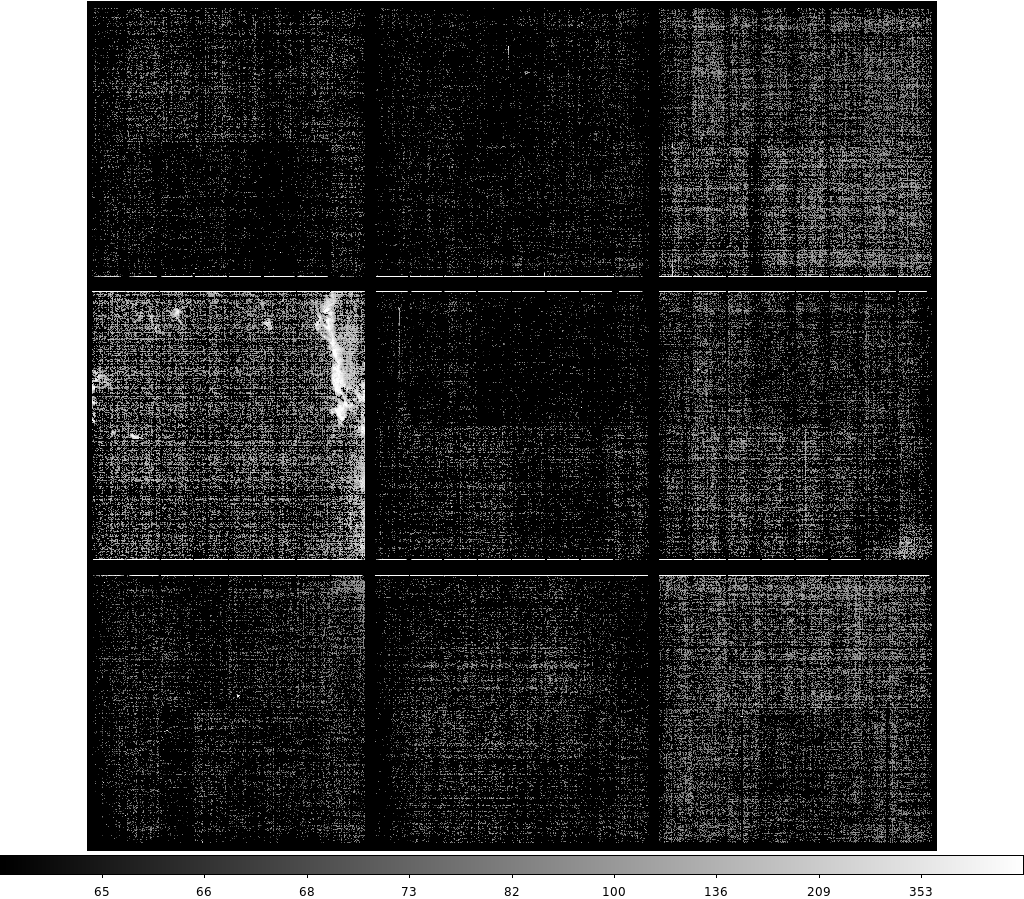
\includegraphics[width=0.9\textwidth]{figures/phosphorescence-survey/itl_fluor_R10_0-19_rb1_log.png}
\caption{Phosphorescence transients for the R10 RTM captured in the first 15\,s following {\it red} CCOB LED at 400\,ke$^-$. With 8$\times$8 blocking, the upper end of the color scale (640) corresponds to 10 e$^-$/pixel when averaged over 64 pixels contributing.}
\label{fig:phos:R10}
\end{figure}

\begin{figure}[!htbp]
\centering
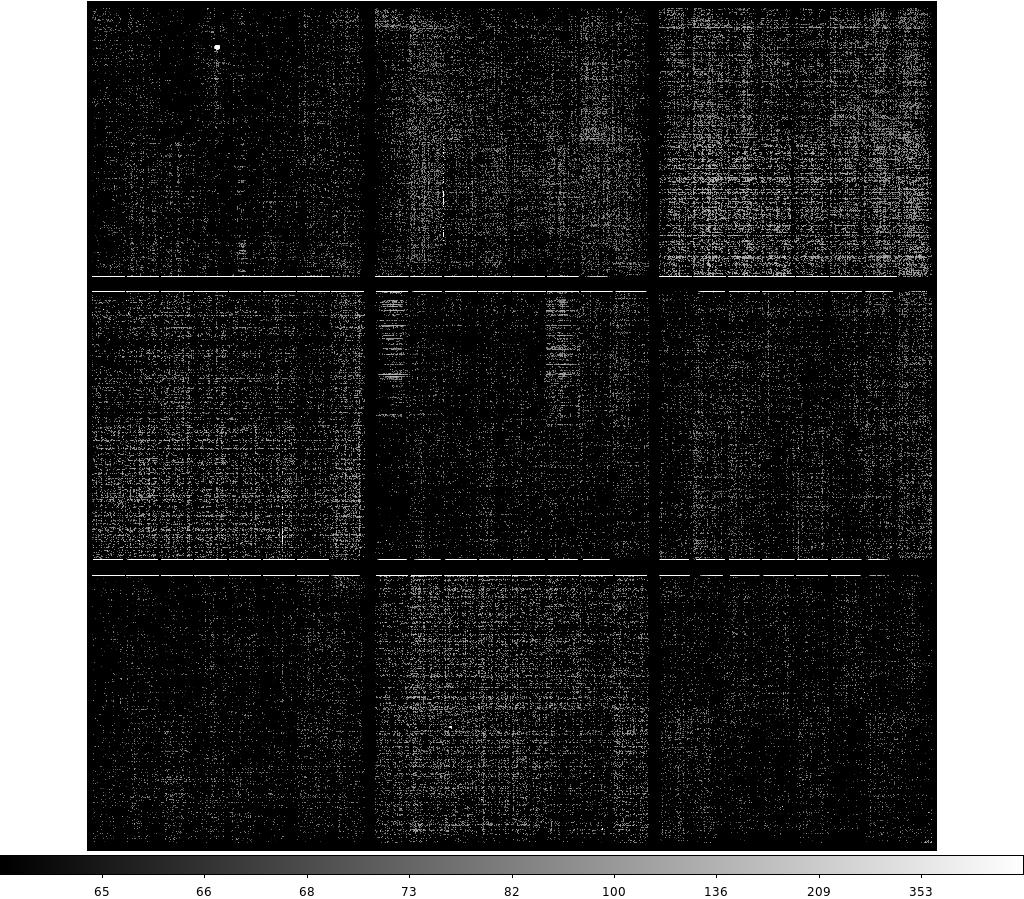
\includegraphics[width=0.9\textwidth]{figures/phosphorescence-survey/itl_fluor_R20_0-19_rb1_log.png}
\caption{Phosphorescence transients for the R20 RTM captured in the first 15\,s following {\it red} CCOB LED at 400\,ke$^-$/pix. With 8$\times$8 blocking, the upper end of the color scale (640) corresponds to 10 e$^-$/pixel when averaged over 64 pixels contributing.}
\label{fig:phos:R20}
\end{figure}

\begin{figure}[!htbp]
\centering
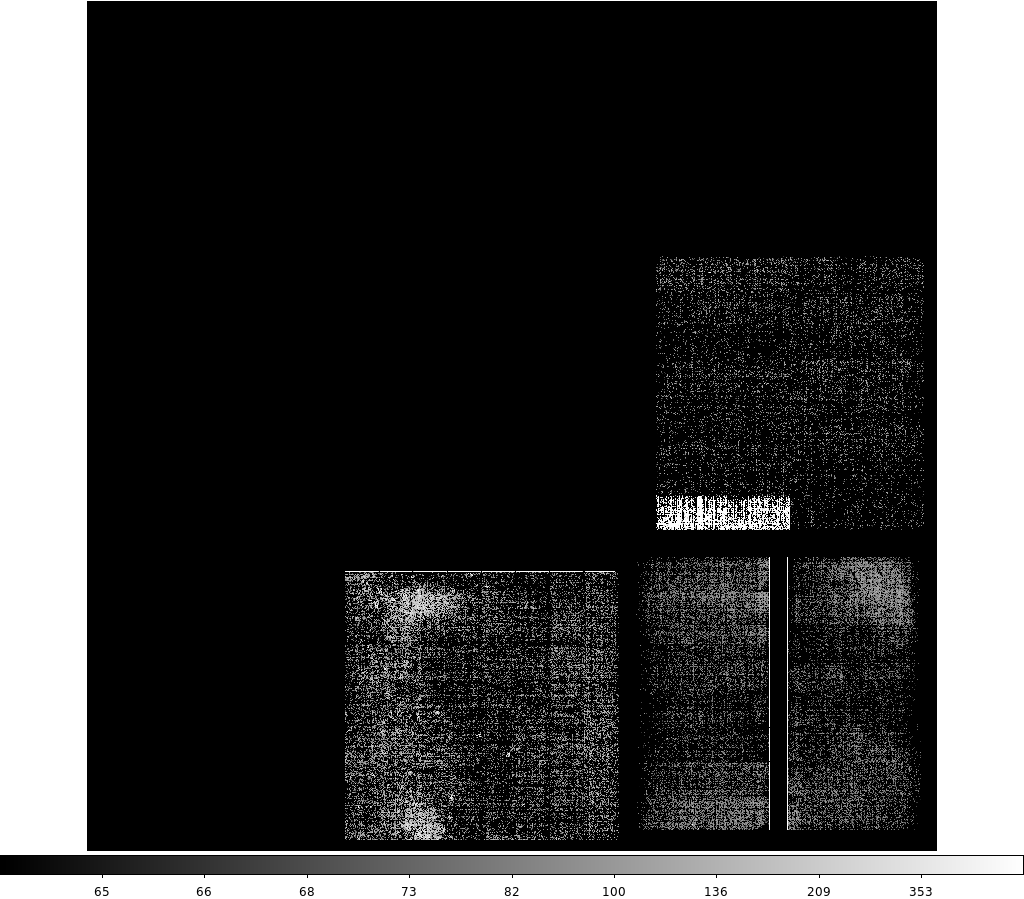
\includegraphics[width=0.9\textwidth]{figures/phosphorescence-survey/itl_fluor_R40_0-19_rb1_log.png}
\caption{Phosphorescence transients for the R40 CRTM captured in the first 15\,s following {\it red} CCOB LED at 400\,ke$^-$/pix. With 8$\times$8 blocking, the upper end of the color scale (640) corresponds to 10 e$^-$/pixel when averaged over 64 pixels contributing.}
\label{fig:phos:R40}
\end{figure}

\begin{figure}[!htbp]
\centering
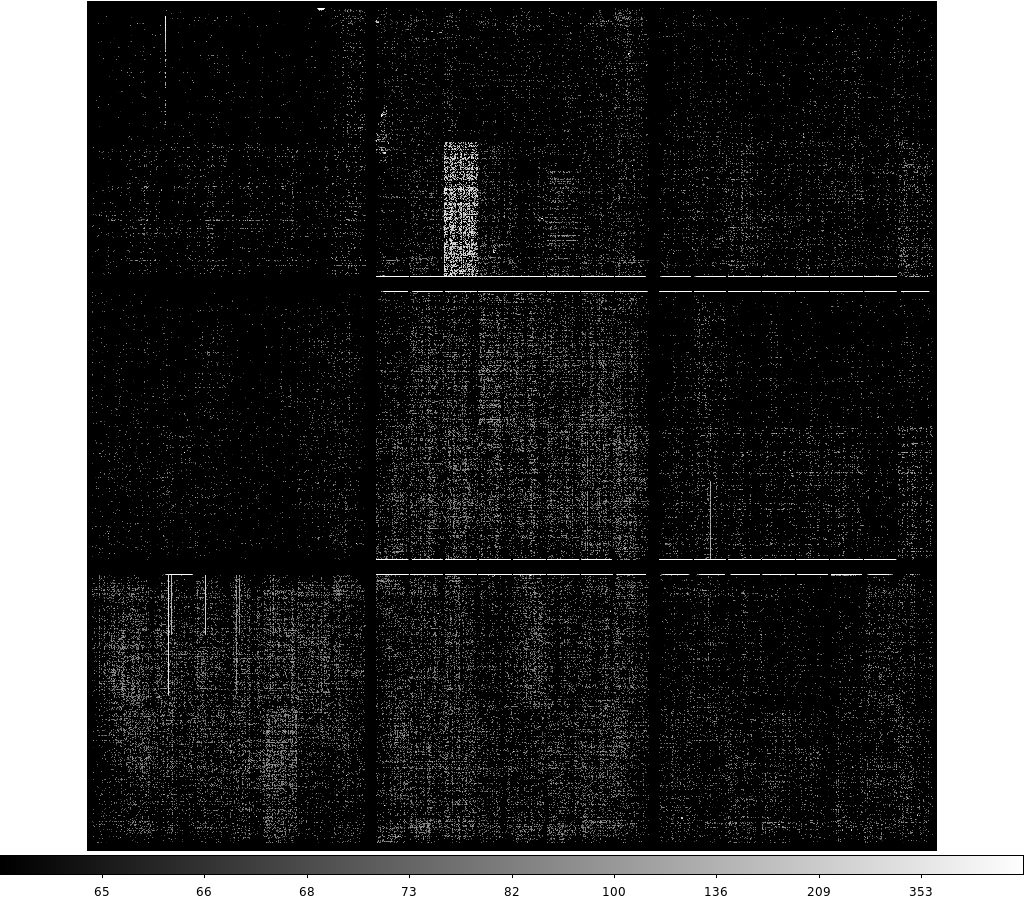
\includegraphics[width=0.9\textwidth]{figures/phosphorescence-survey/itl_fluor_R41_0-19_rb1_log.png}
\caption{Phosphorescence transients for the R41 RTM captured in the first 15\,s following {\it red} CCOB LED at 400\,ke$^-$/pix. With 8$\times$8 blocking, the upper end of the color scale (640) corresponds to 10 e$^-$/pixel when averaged over 64 pixels contributing.}
\label{fig:phos:R41}
\end{figure}

\begin{figure}[!htbp]
\centering
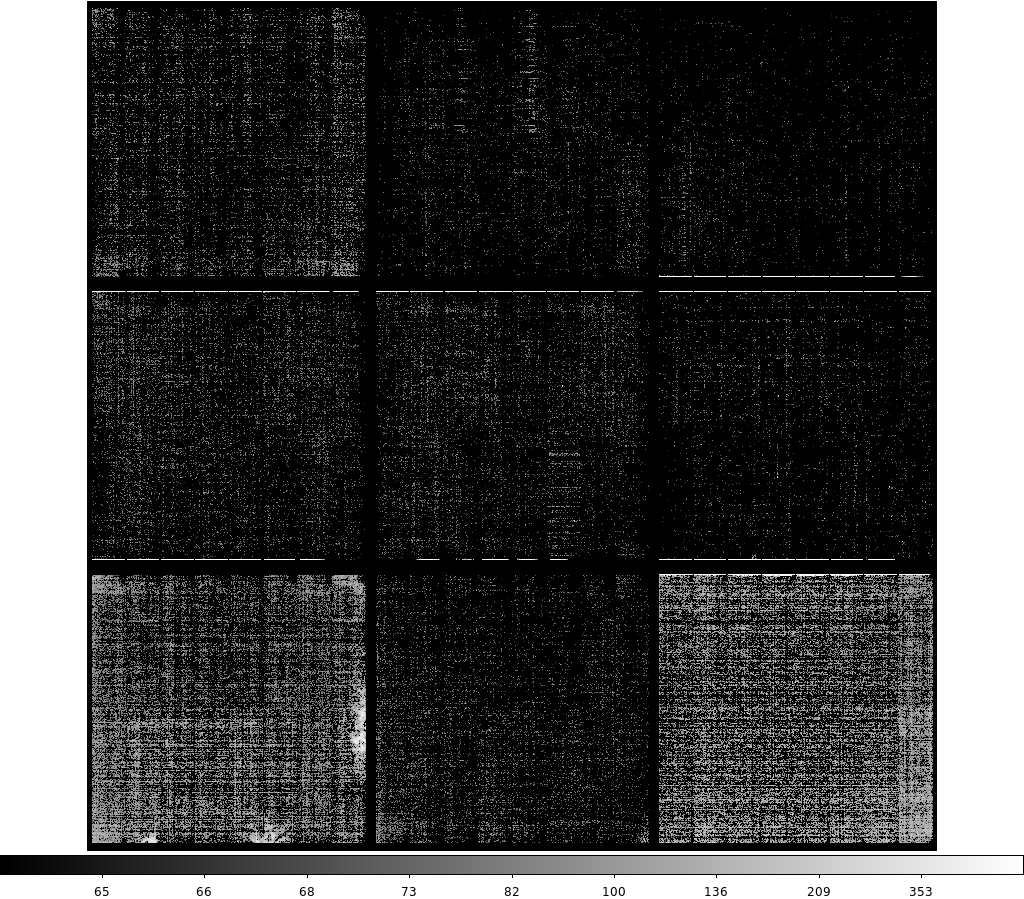
\includegraphics[width=0.9\textwidth]{figures/phosphorescence-survey/itl_fluor_R42_0-19_rb1_log.png}
\caption{Phosphorescence transients for the R42 RTM captured in the first 15\,s following {\it red} CCOB LED at 400\,ke$^-$/pix. With 8$\times$8 blocking, the upper end of the color scale (640) corresponds to 10 e$^-$/pixel when averaged over 64 pixels contributing.}
\label{fig:phos:R42}
\end{figure}

\begin{figure}[!htbp]
\centering
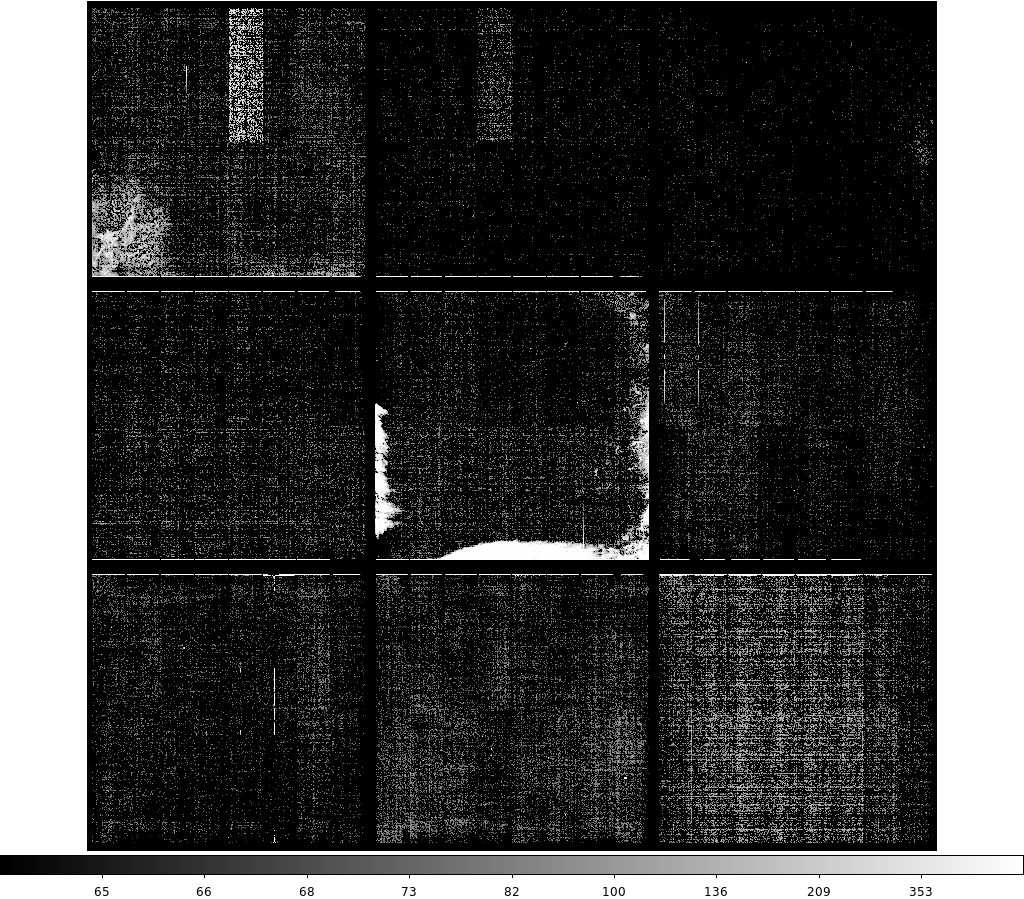
\includegraphics[width=0.9\textwidth]{figures/phosphorescence-survey/itl_fluor_R43_0-19_rb1_log.png}
\caption{Phosphorescence transients for the R43 RTM captured in the first 15\,s following {\it red} CCOB LED at 400\,ke$^-$/pix. With 8$\times$8 blocking, the upper end of the color scale (640) corresponds to 10 e$^-$/pixel when averaged over 64 pixels contributing.}
\label{fig:phos:R43}
\end{figure}

\begin{figure}[!htbp]
\centering
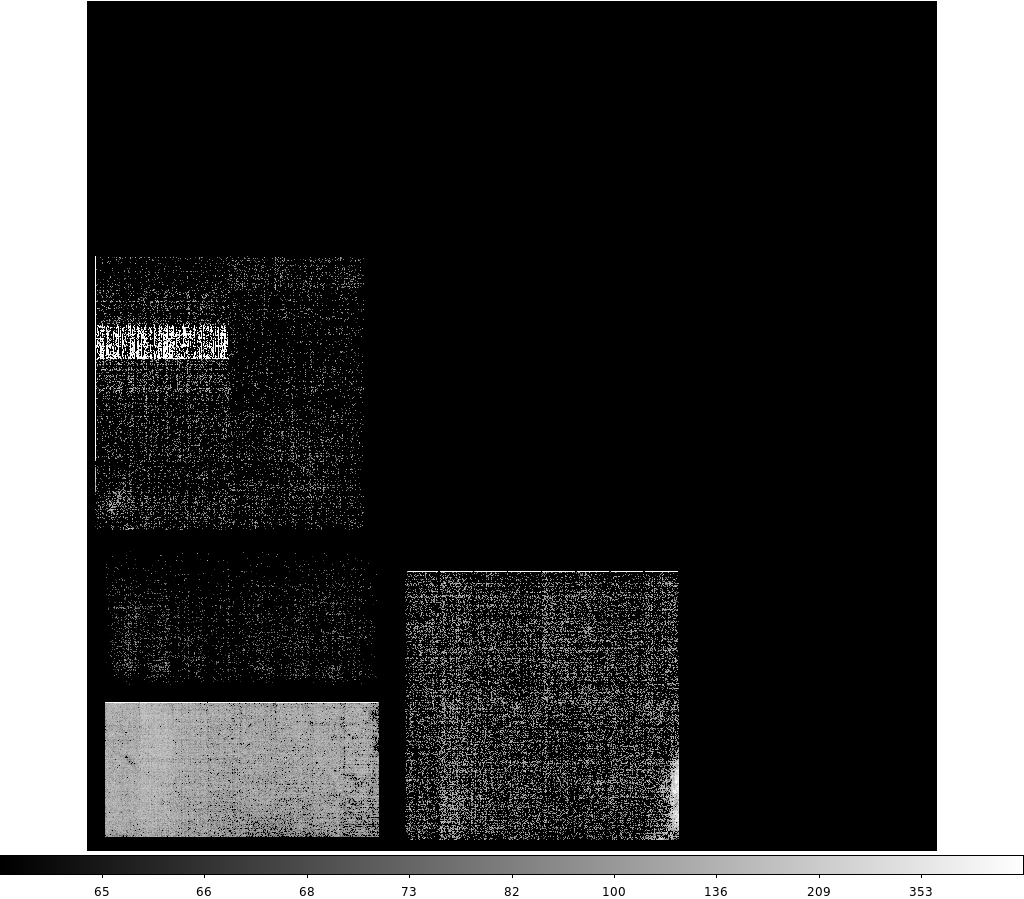
\includegraphics[width=0.9\textwidth]{figures/phosphorescence-survey/itl_fluor_R44_0-19_rb1_log.png}
\caption{Phosphorescence transients for the R44 CRTM captured in the first 15\,s following {\it red} CCOB LED at 400\,ke$^-$/pix. With 8$\times$8 blocking, the upper end of the color scale (640) corresponds to 10 e$^-$/pixel when averaged over 64 pixels contributing.}
\label{fig:phos:R44}
\end{figure}

\clearpage
\section{Phosphorescence morphological comparisons with features seen in {\it blue} flat field response}

The following images (Figures~\ref{fig:phos:stains:R01S00} through \ref{fig:phos:stains:R43S20}) are an incomplete selection of ITL sensors with phosphorescence. They compare expressed phosphorescence (transient term) with the {\it blue} CCOB LED flat response.

\begin{figure}[!htbp]
\centering
\begin{minipage}{1.0\textwidth}    
  \centering
  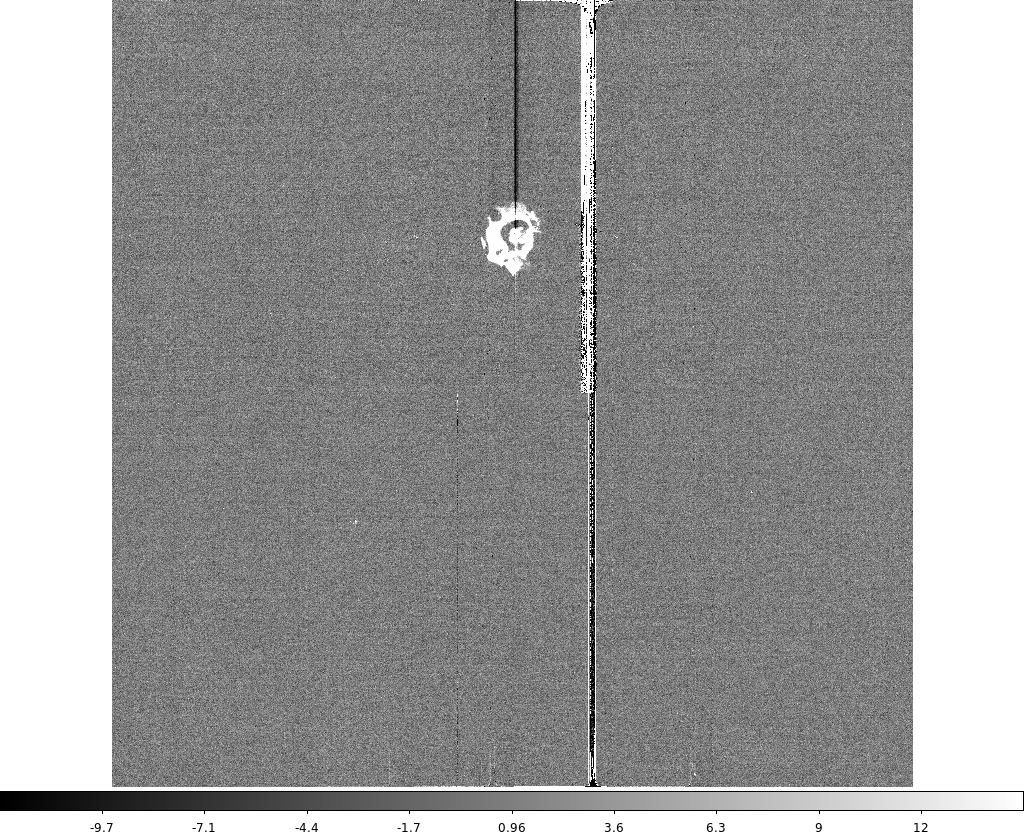
\includegraphics[width=.6\linewidth]{figures/phosphorescence-survey/stains_phos_R01_S00.png}    
\end{minipage}
\begin{minipage}{1.0\textwidth}
  \centering
  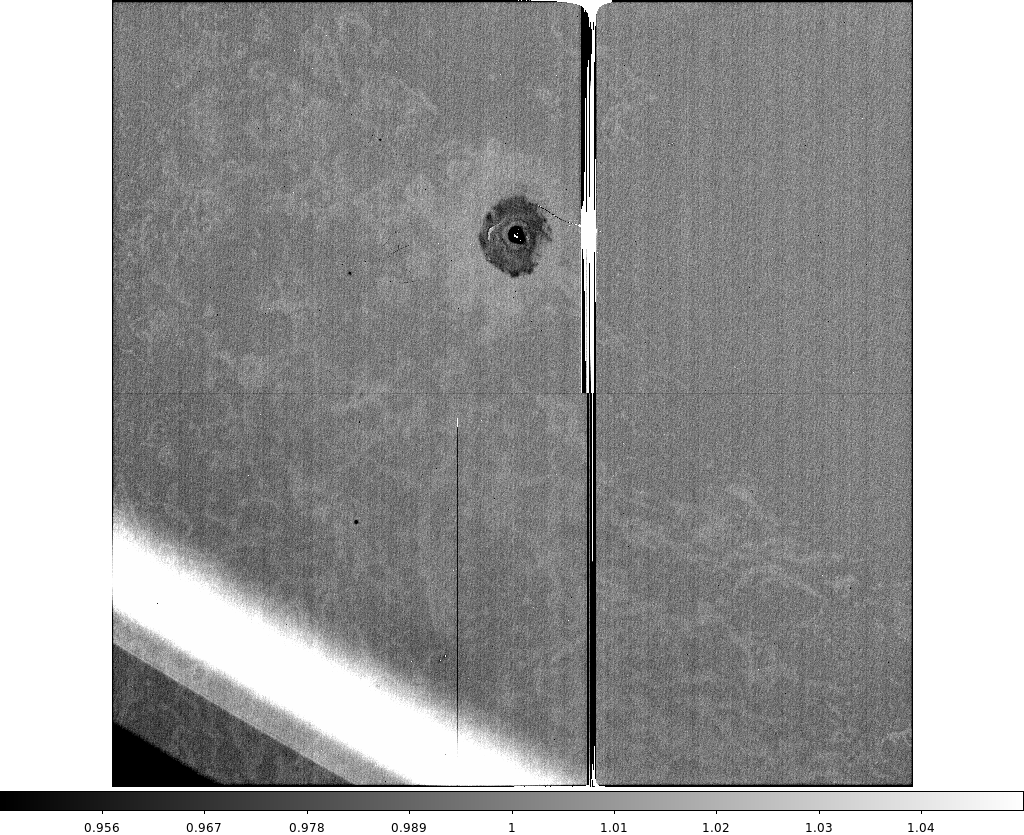
\includegraphics[width=.6\linewidth]{figures/phosphorescence-survey/stains_abs_R01_S00.png}
\end{minipage}
\caption{The ITL sensor R01\_S00. Top: the transient phosphorescence term. Bottom: the {\it blue} flat response. The large, extended spot appears to be centered on a {\it vampire pixel}, which also expresses a large amplitude of phosphorescence, which emits enough current to contaminate the parallel overscan in at least the first 15\,s exposure following trigger. The flat response feature has opposite polarity from the phosphorescence.}
\label{fig:phos:stains:R01S00}
\end{figure}


\begin{figure}[!htbp]
\centering
\begin{minipage}{1.0\textwidth}    
  \centering
  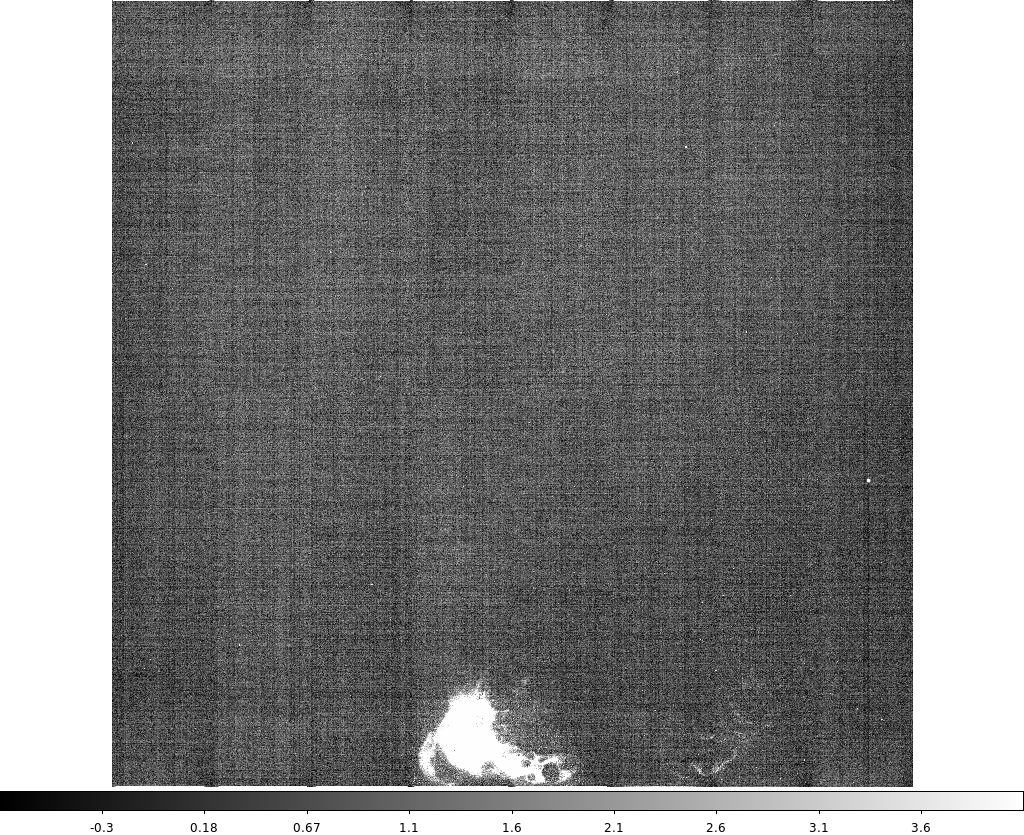
\includegraphics[width=.6\linewidth]{figures/phosphorescence-survey/stains_phos_R02_S02.png}    
\end{minipage}
\begin{minipage}{1.0\textwidth}
  \centering
  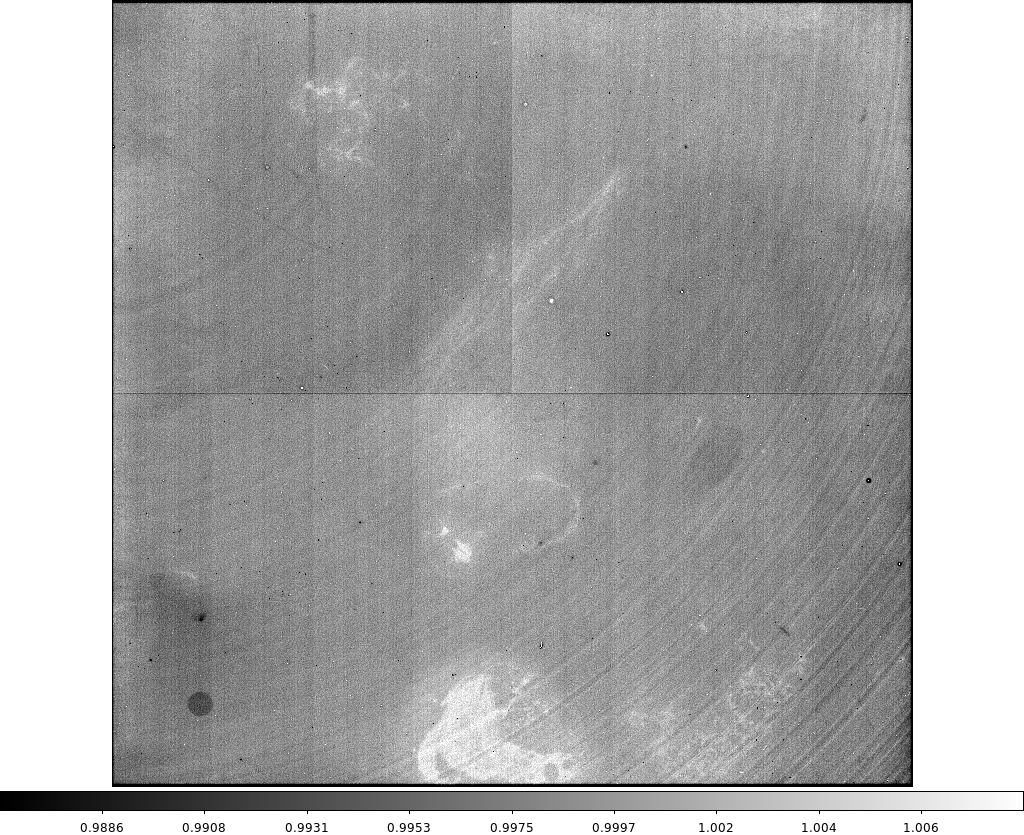
\includegraphics[width=.6\linewidth]{figures/phosphorescence-survey/stains_abs_R02_S02.png}
\end{minipage}
\caption{The ITL sensor R02\_S02. Top: the transient phosphorescence term. Bottom: the {\it blue} flat response. The {\it coffee stain} feature in the flat response has the same polarity as the phosphorescence. A phosphorescent {\it vampire pixel} is seen in segment R02\_S02\_C07.}
\label{fig:phos:stains:R02S02}
\end{figure}

\begin{figure}[!htbp]
\centering
\begin{minipage}{1.0\textwidth}    
  \centering
  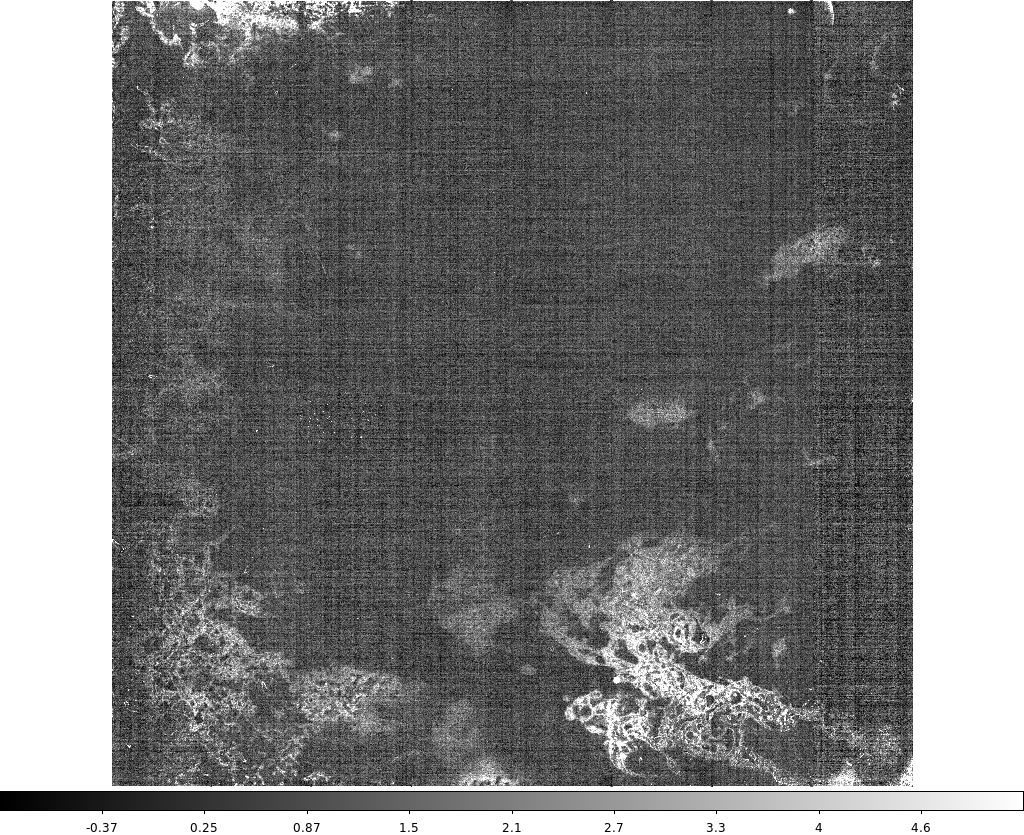
\includegraphics[width=.6\linewidth]{figures/phosphorescence-survey/stains_phos_R02_S12.png}    
\end{minipage}
\begin{minipage}{1.0\textwidth}
  \centering
  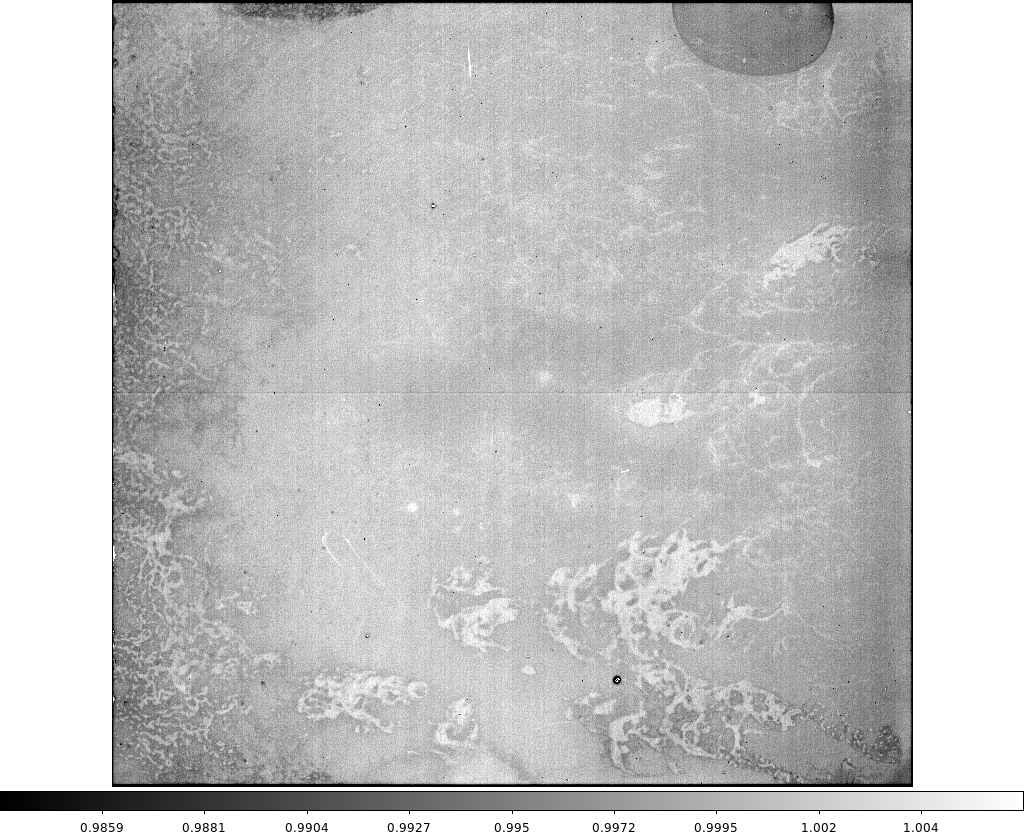
\includegraphics[width=.6\linewidth]{figures/phosphorescence-survey/stains_abs_R02_S12.png}
\end{minipage}
\caption{The ITL sensor R02\_S12. Top: the transient phosphorescence term. Bottom: the {\it blue} flat response. Generally the polarity of the phosphorescence matches that of the {\it coffee stain} in the flat field response, but exceptions include the {\it vampire pixel} seen in segment R02\_S12\_C05.}
\label{fig:phos:stains:R02S12}
\end{figure}


\begin{figure}[!htbp]
\centering
\begin{minipage}{1.0\textwidth}    
  \centering
  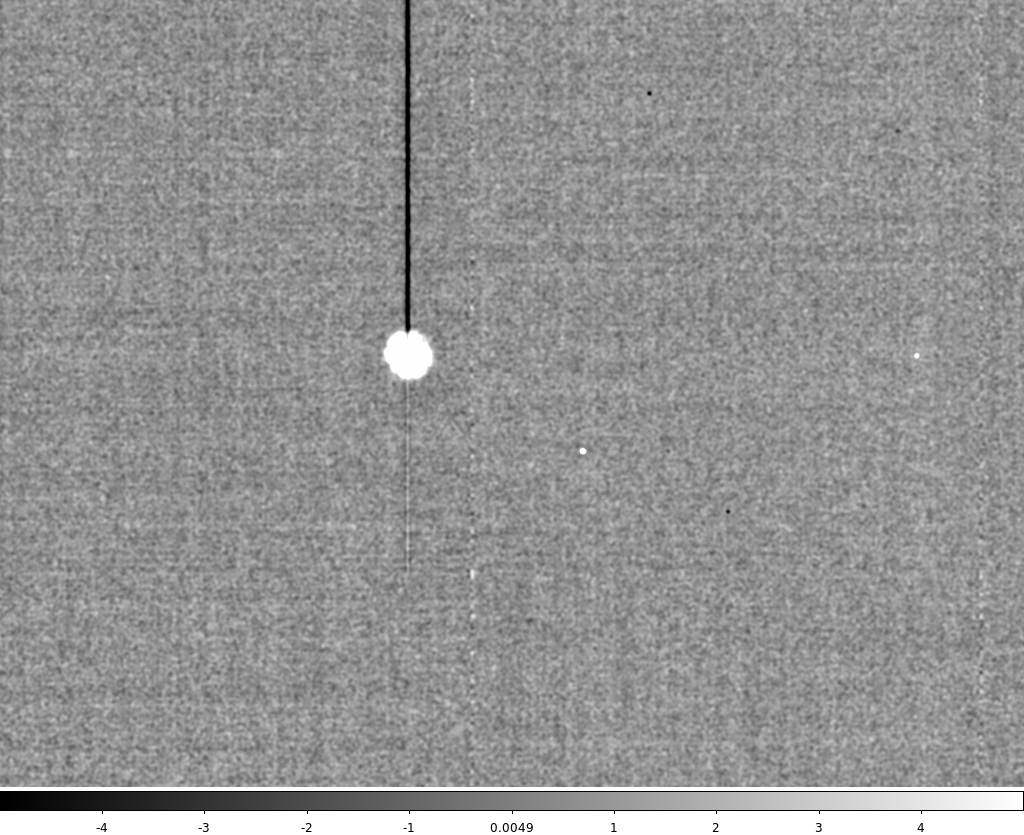
\includegraphics[width=.6\linewidth]{figures/phosphorescence-survey/stains_phos_R03_S10.png}    
\end{minipage}
\begin{minipage}{1.0\textwidth}
  \centering
  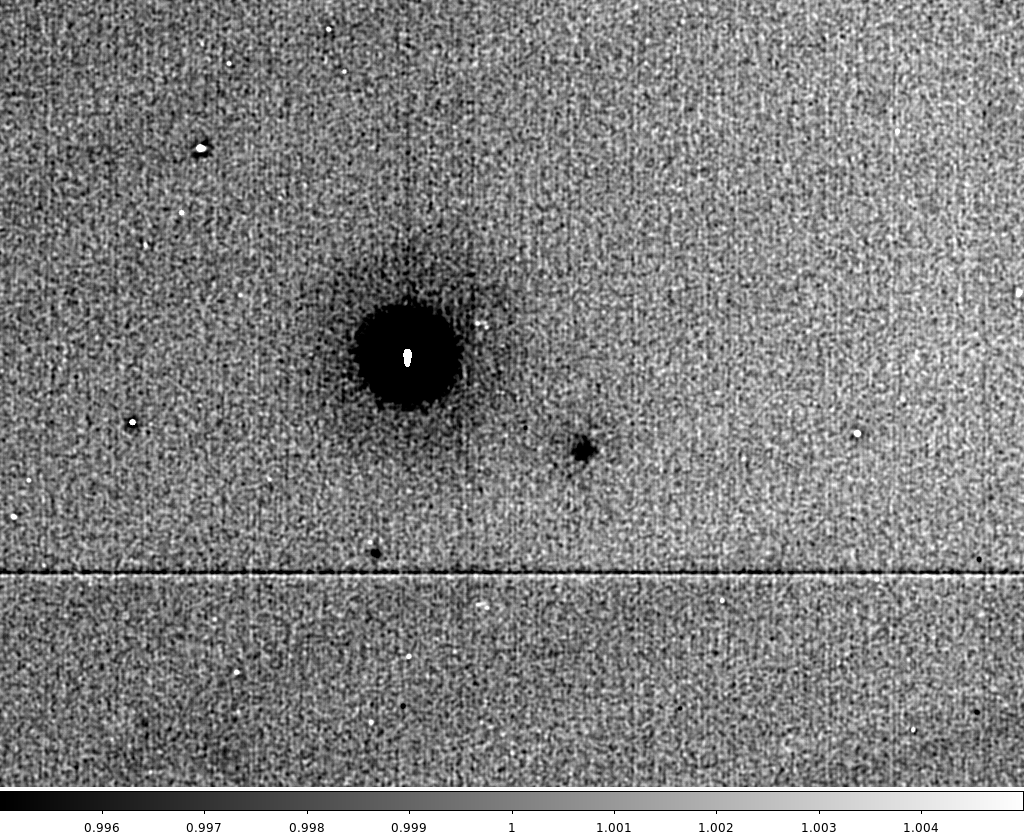
\includegraphics[width=.6\linewidth]{figures/phosphorescence-survey/stains_abs_R03_S10.png}
\end{minipage}
\caption{The ITL sensor R03\_S10, detail of the {\it vampire pixel} of R03\_S10\_C15. Top: the transient phosphorescence term. Bottom: the {\it blue} flat response. As in previous examples, this {\it vampire pixel}'s transient term is large enough to contaminate the parallel overscan even after the first 15\,s following trigger.}
\label{fig:phos:stains:R03S10}
\end{figure}


\begin{figure}[!htbp]
\centering
\begin{minipage}{1.0\textwidth}    
  \centering
  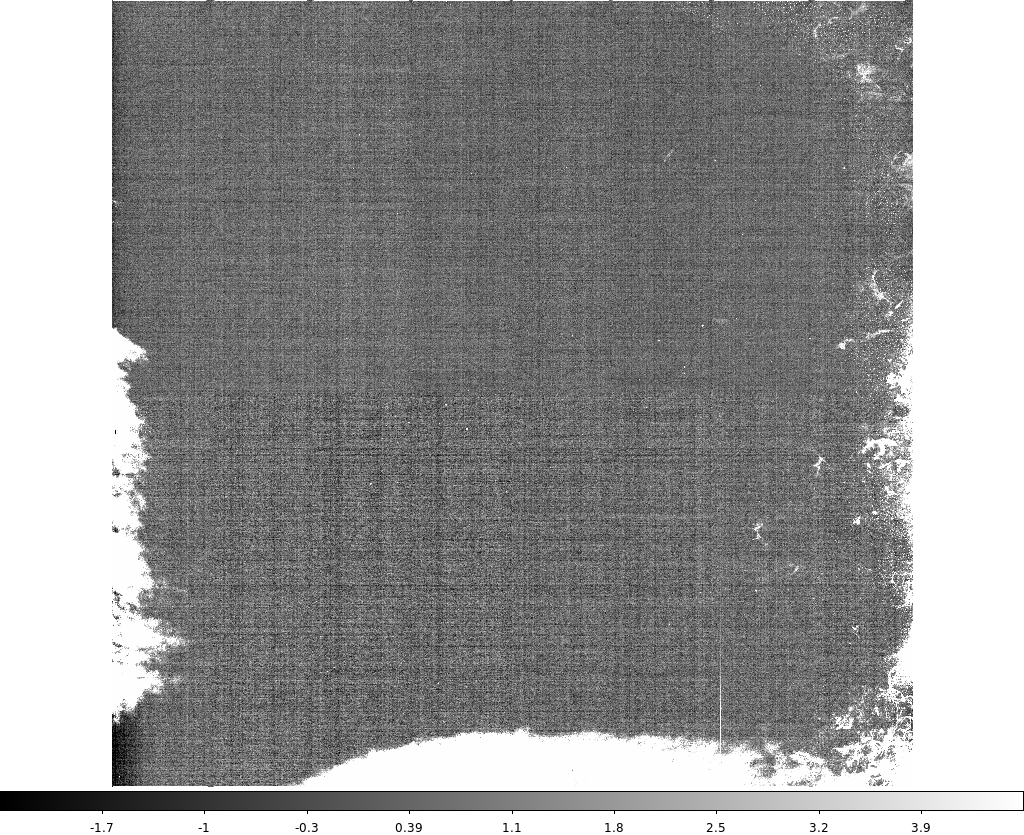
\includegraphics[width=.6\linewidth]{figures/phosphorescence-survey/stains_phos_R43_S11.png}    
\end{minipage}
\begin{minipage}{1.0\textwidth}
  \centering
  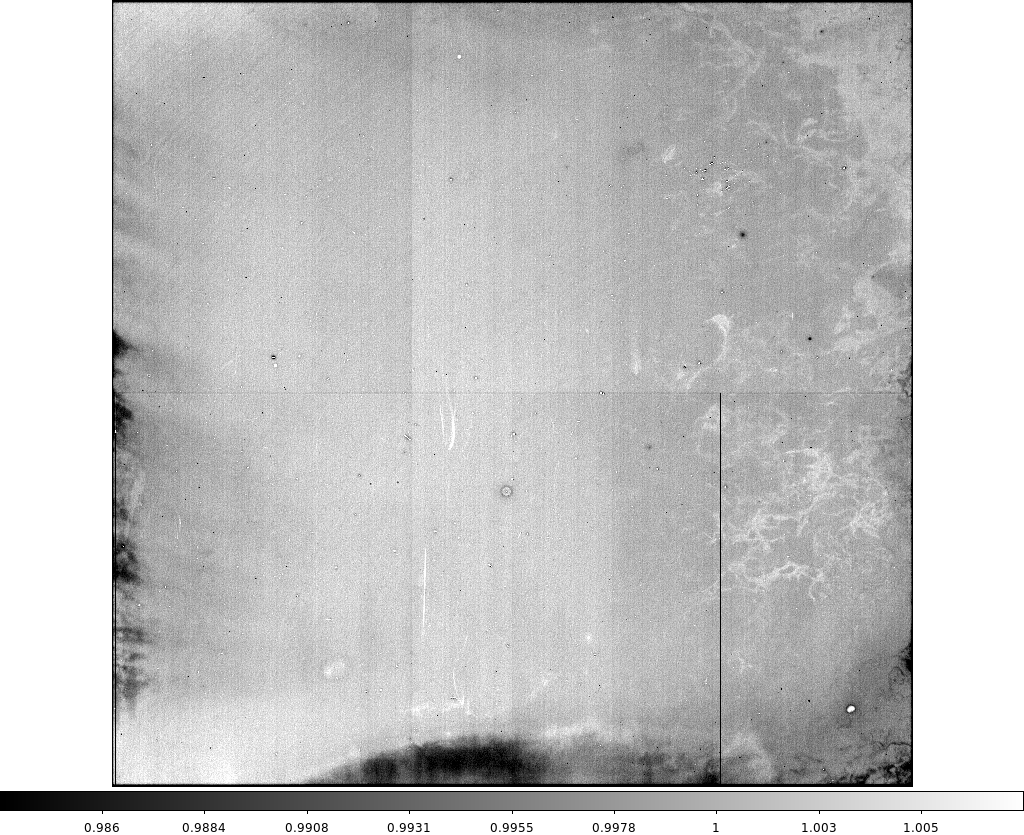
\includegraphics[width=.6\linewidth]{figures/phosphorescence-survey/stains_abs_R43_S11.png}
\end{minipage}
\caption{The ITL sensor R43\_S11. Top: the transient phosphorescence term. Bottom: the {\it blue} flat response. This sensor appears to have the largest integrated phosphorescence among ITL sensors studied. The flat response feature has opposite polarity from the phosphorescence.}
\label{fig:phos:stains:R43S11}
\end{figure}


\begin{figure}[!htbp]
\centering
\begin{minipage}{1.0\textwidth}    
  \centering
  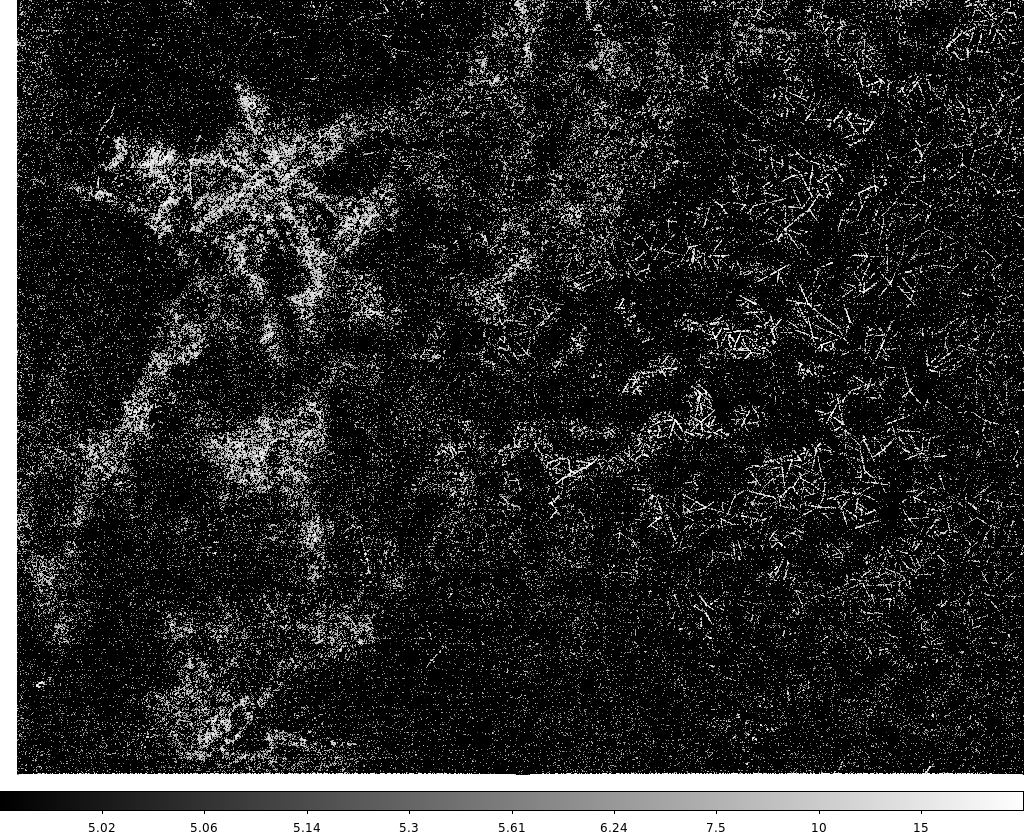
\includegraphics[width=.6\linewidth]{figures/phosphorescence-survey/stains_phos_R43_S20_detail.png}    
\end{minipage}
\begin{minipage}{1.0\textwidth}
  \centering
  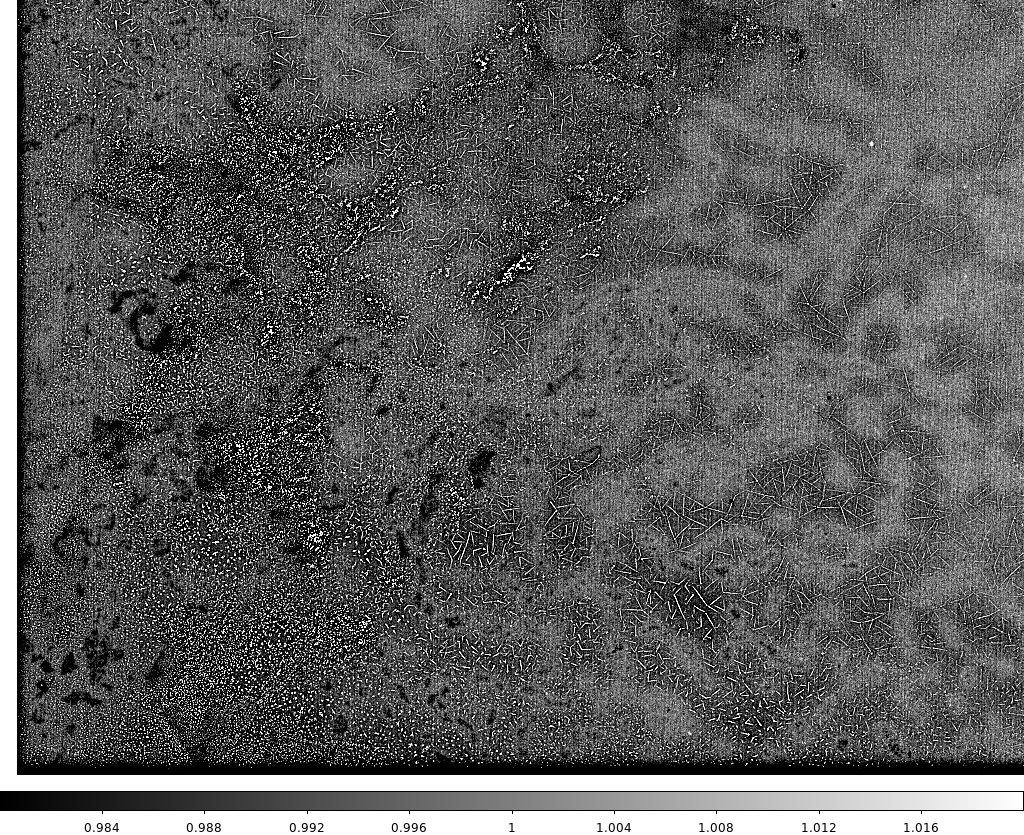
\includegraphics[width=.6\linewidth]{figures/phosphorescence-survey/stains_abs_R43_S20_detail.png}
\end{minipage}
\caption{The ITL sensor R43\_S20, segments C00 through C03. Top: the transient phosphorescence term. Bottom: the {\it blue} flat response. This sensor apparently exhibits peculiar radial crazing patterns seen in both phosphorescence as well as in flat field response, with polarities aligned.}
\label{fig:phos:stains:R43S20}
\end{figure}

\clearpage
\section{Phosphorescence kinetics characterization}
\label{sect:kinetics}
Figures~\ref{fig:phos:kinetics:R01S00} through \ref{fig:phos:kinetics:R43S20} quantify the expressed phosphorescence distributions in ROIs on seven of the problematic ITL sensors. Previously, we had captured the phosphorescence {\it transient term} across the ITL sensors ({\it cf.} Figs.~\ref{fig:phos:R00} thru \ref{fig:phos:R44}); here we track ROI pixel distribution parameters of individual median images constructed from the selection of specific images acquired across the 20 B-protocol datasets available (listed in Table~\ref{tab:phosphorescence:datasets}). 

By fitting decay models to these persistence curves, it is immediately clear that there are multiple (>2) timescales at play for the pixels in each ROI. An example of such a fit is given in Figure~\ref{fig:phos:kinetics:fit:R20S20C13} where a 3-population relaxation model is used to characterize evolution of the 99\% quantile level of the distribution. In this case, there are three different exponential timescales determined: $(\tau_1,\tau_2,\tau_3) = (0.62,2.5,18.3)$ in image units (10.9, 43.8 \& 320 seconds, respectively). The corresponding ratio of these populations works out to 4.5\% (fast), 21.5\% (medium) and 74\% (slow), respectively. Inspection of the more detailed parameters plotted generally indicate skewed distributions from mismatches between medians and means; the choice of the 99\% quantile level to characterize was mainly to estimate the degree to which images would need to be phosphorescence-corrected (and/or the variance plane modified, given the asymmetric impact of the position specific, phosphorescence contribution in recorded images). 

\begin{figure}[!htbp]
\centering
\begin{subfigure}{0.8\textwidth}    
  \centering
  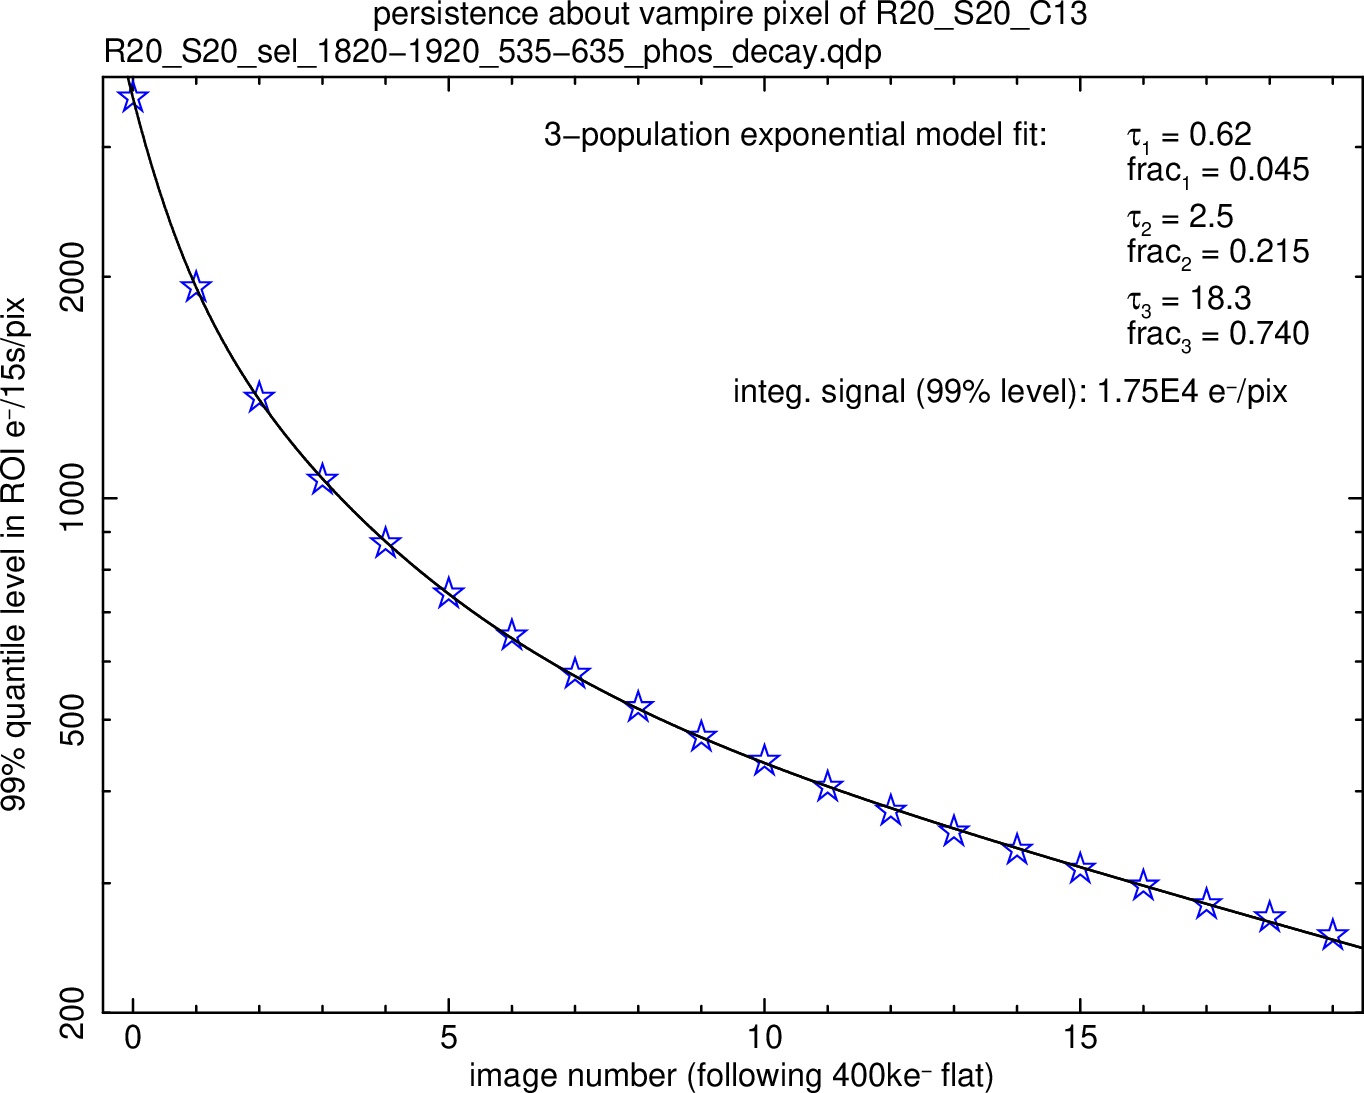
\includegraphics[width=\textwidth]{figures/phosphorescence-survey/phos_kinetics/R20_S20_sel_1820-1920_535-635_phos_decay_fit.png}    
\end{subfigure}
\caption{A three-population fit of the phosphorescence expressed by the vapire pixel region of R20\_S20\_C13. The fit was performed on the 99\% quantile level where signal levels are well above the $3\sigma$ level of the noise distribution. Here, image numbers are parasitically used as time units, with roughly 17.5 seconds per image.}
\label{fig:phos:kinetics:fit:R20S20C13}
\end{figure}

\begin{figure}[!htbp]
\begin{subfigure}{0.45\textwidth}    
  \centering
  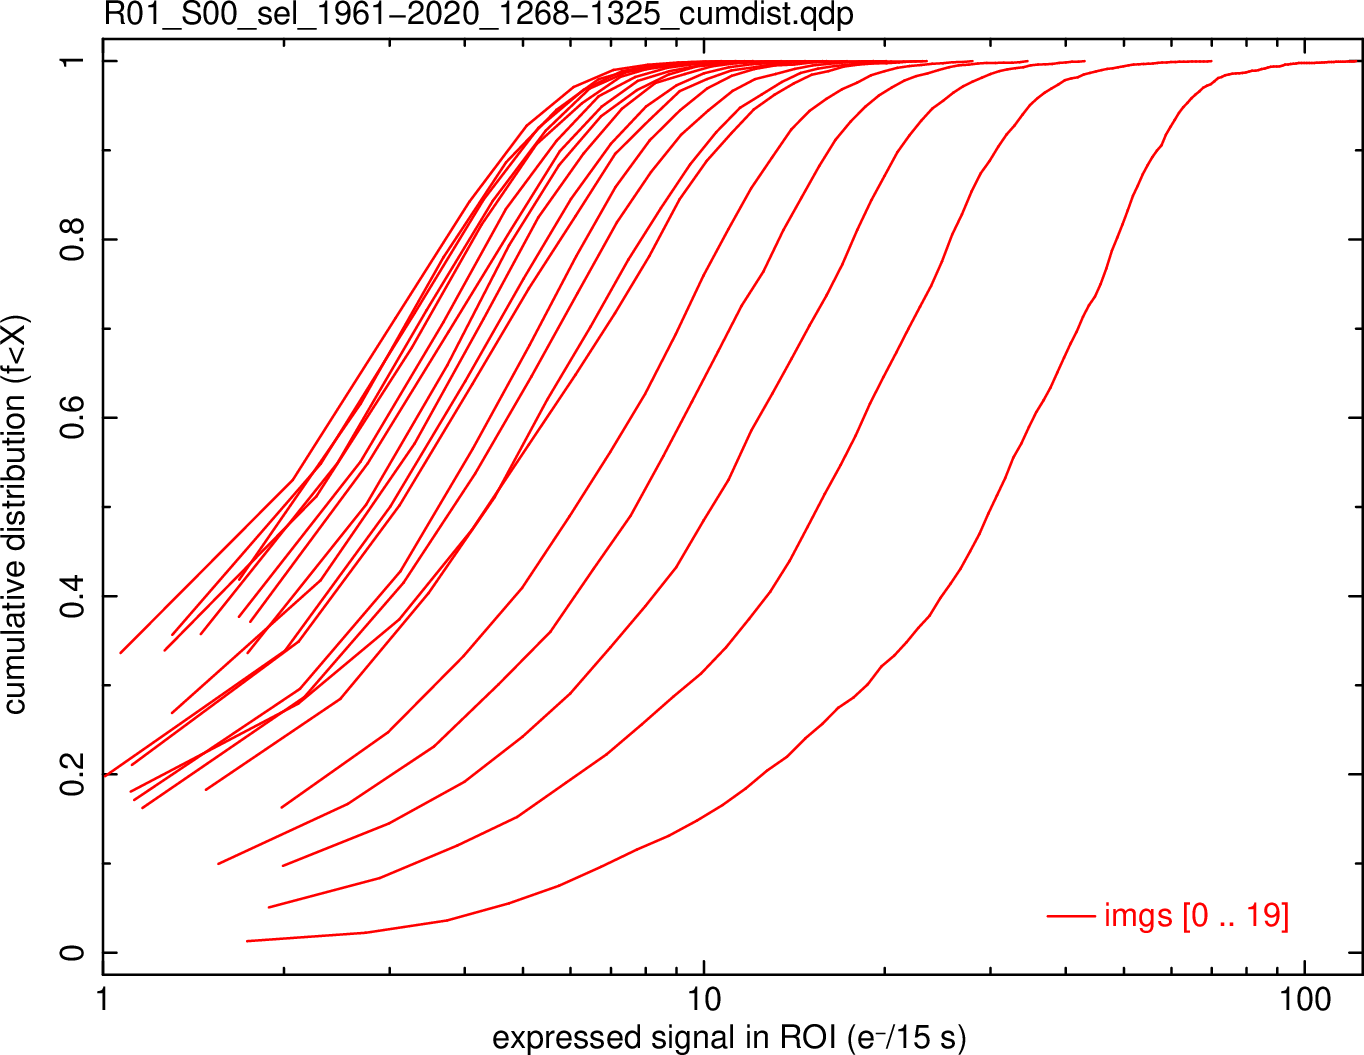
\includegraphics[width=\textwidth]{figures/phosphorescence-survey/phos_kinetics/R01_S00_sel_1961-2020_1268-1325_cumdist.png}    
\end{subfigure}
\hfil
\begin{subfigure}{0.45\textwidth}
  \centering
  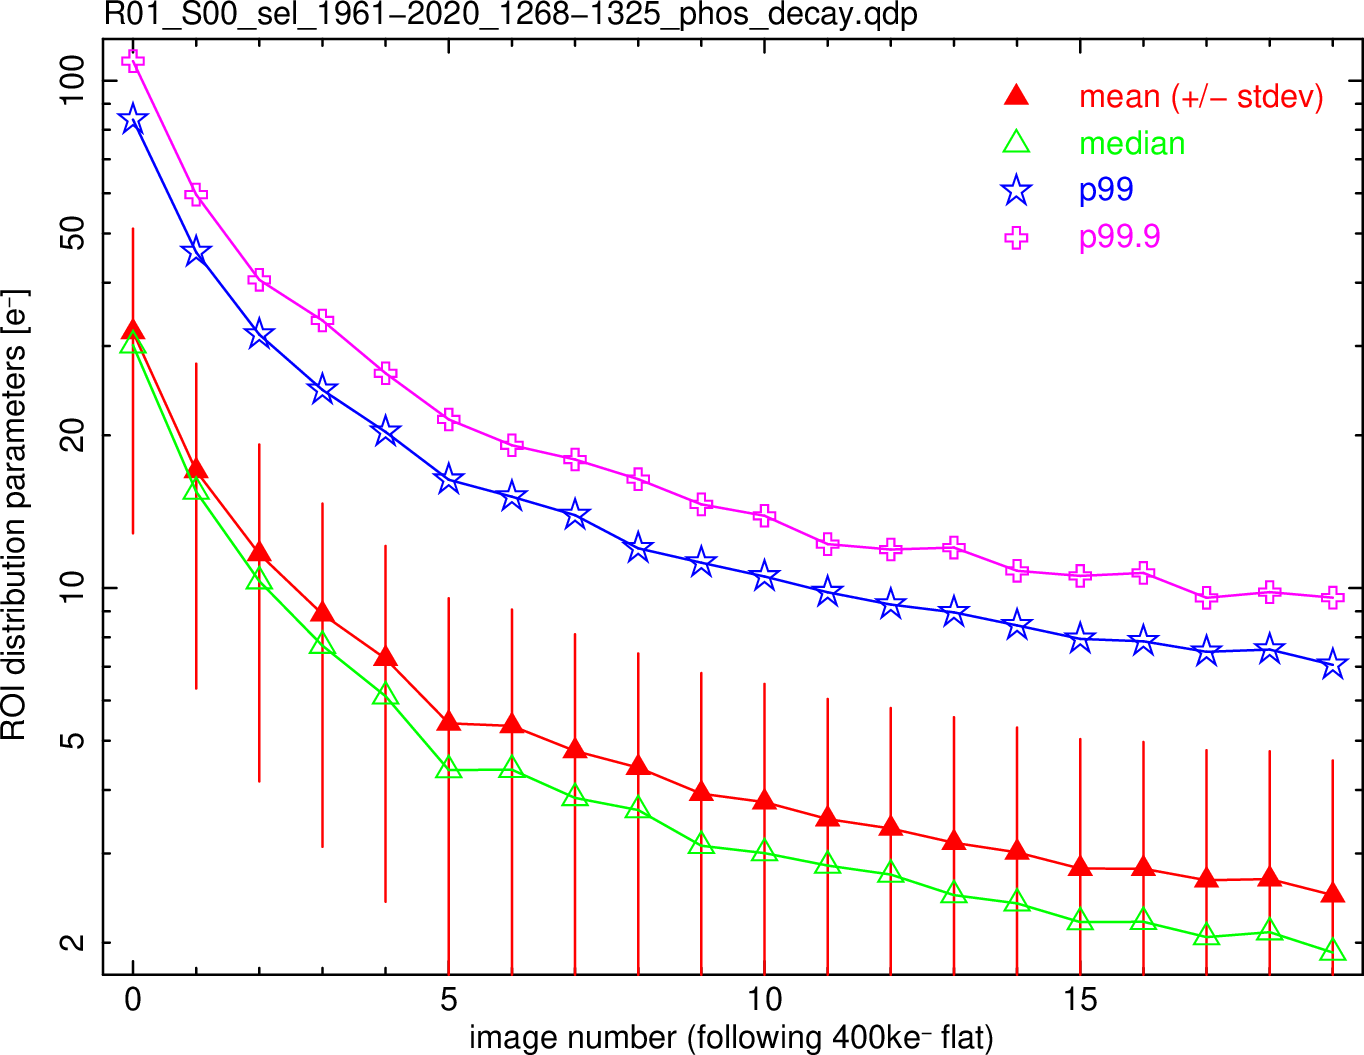
\includegraphics[width=\textwidth]{figures/phosphorescence-survey/phos_kinetics/R01_S00_sel_1961-2020_1268-1325_phos_decay.png}
\end{subfigure}
\newline
\begin{subfigure}{0.45\textwidth}    
  \centering
  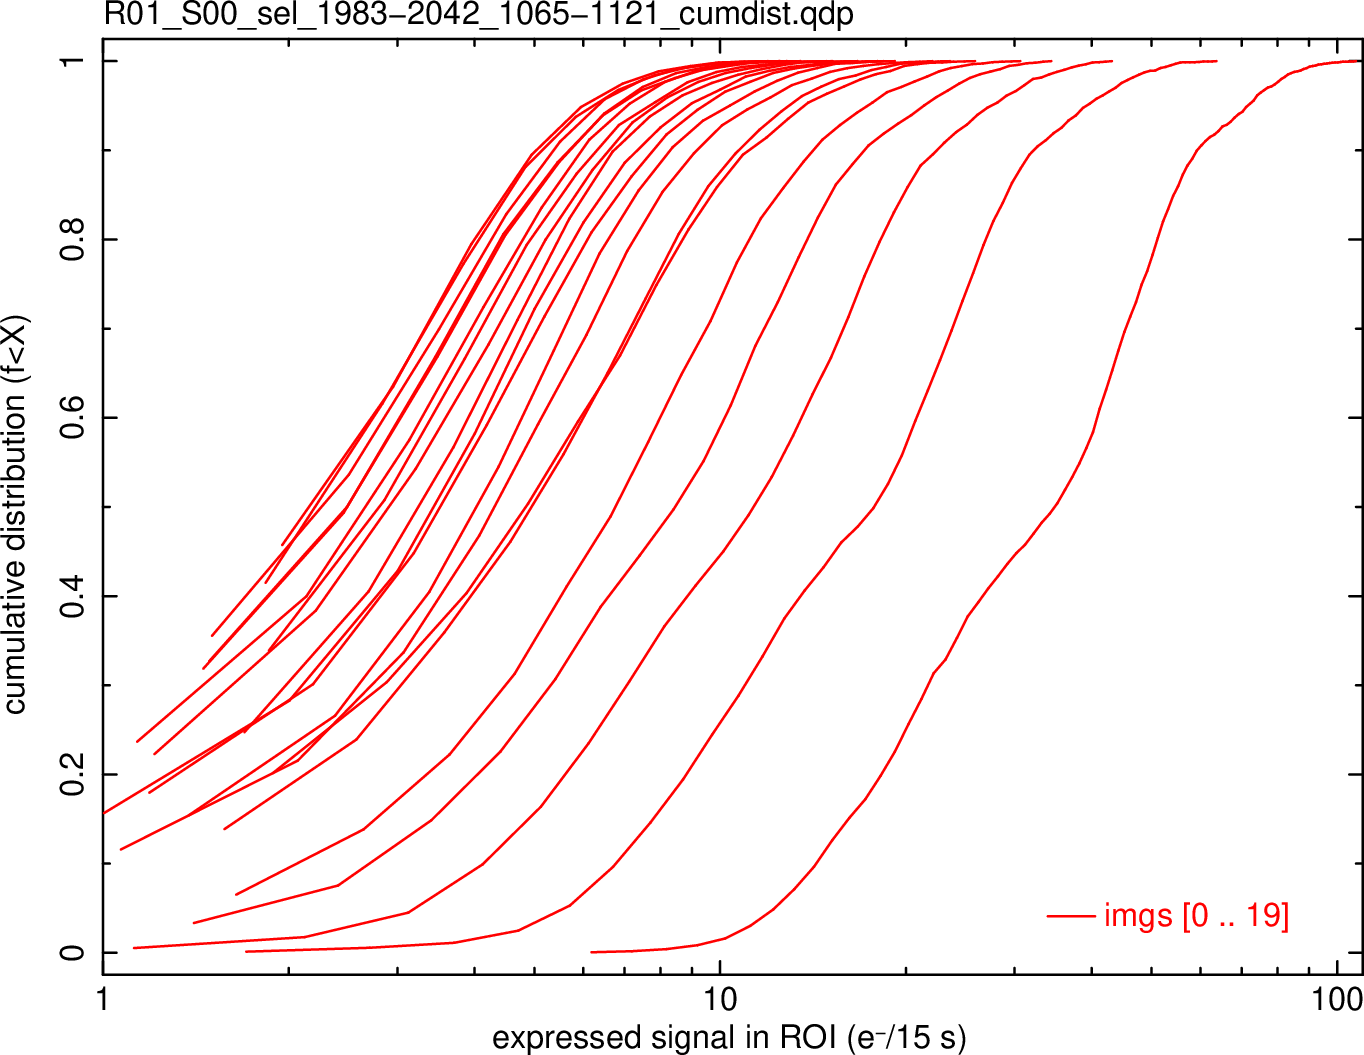
\includegraphics[width=\textwidth]{figures/phosphorescence-survey/phos_kinetics/R01_S00_sel_1983-2042_1065-1121_cumdist.png}    
\end{subfigure}
\hfil
\begin{subfigure}{0.45\textwidth}
  \centering
  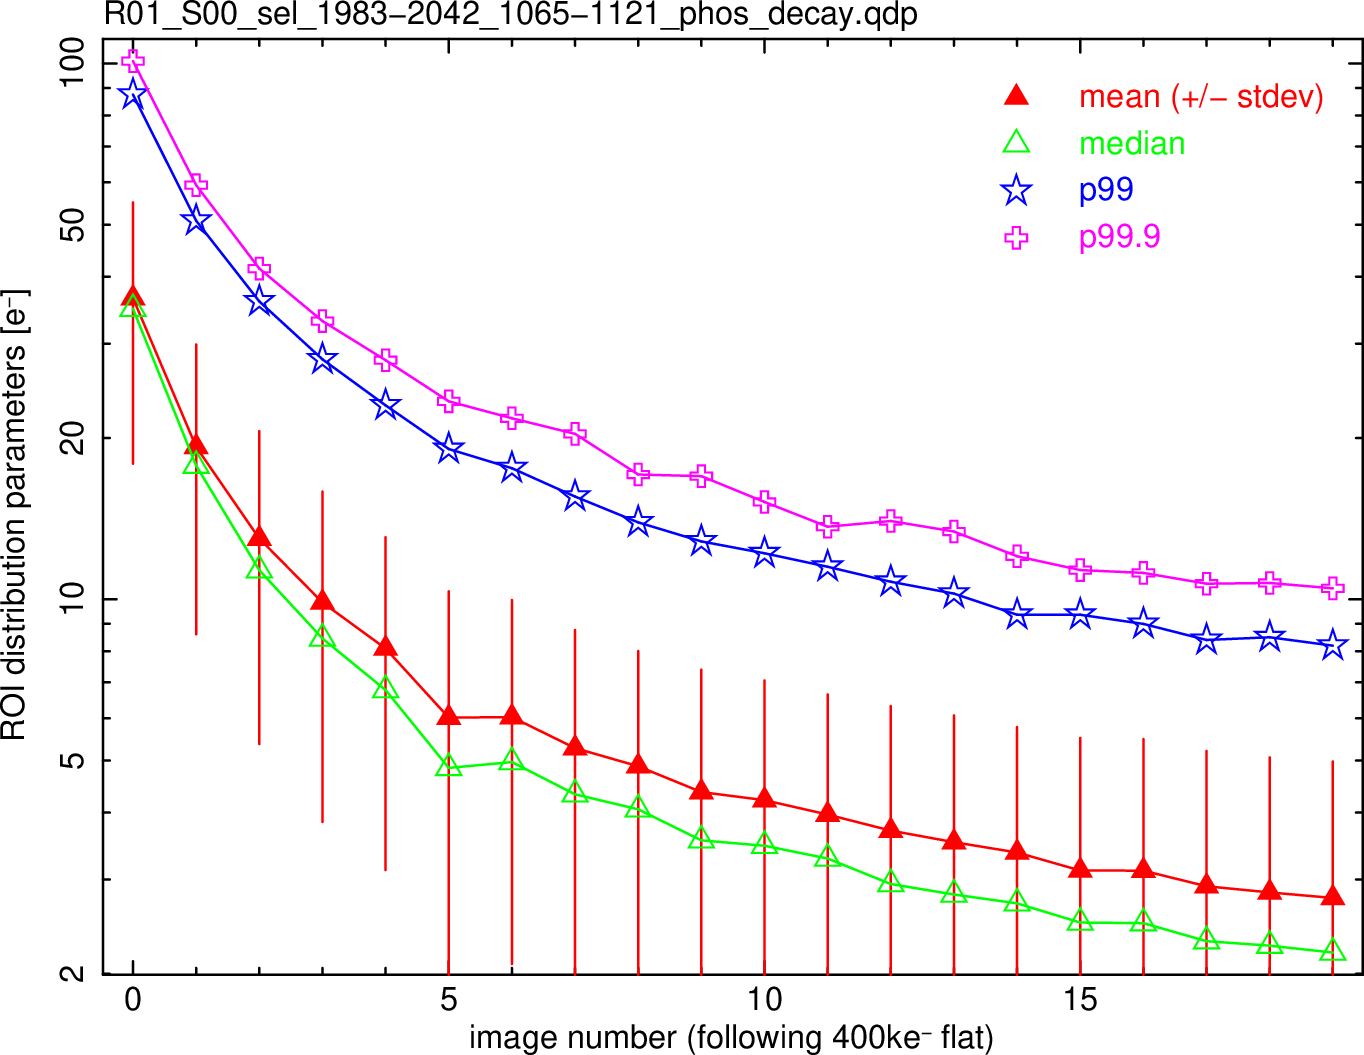
\includegraphics[width=\textwidth]{figures/phosphorescence-survey/phos_kinetics/R01_S00_sel_1983-2042_1065-1121_phos_decay.png}
\end{subfigure}
\newline
\begin{subfigure}{0.45\textwidth}    
  \centering
  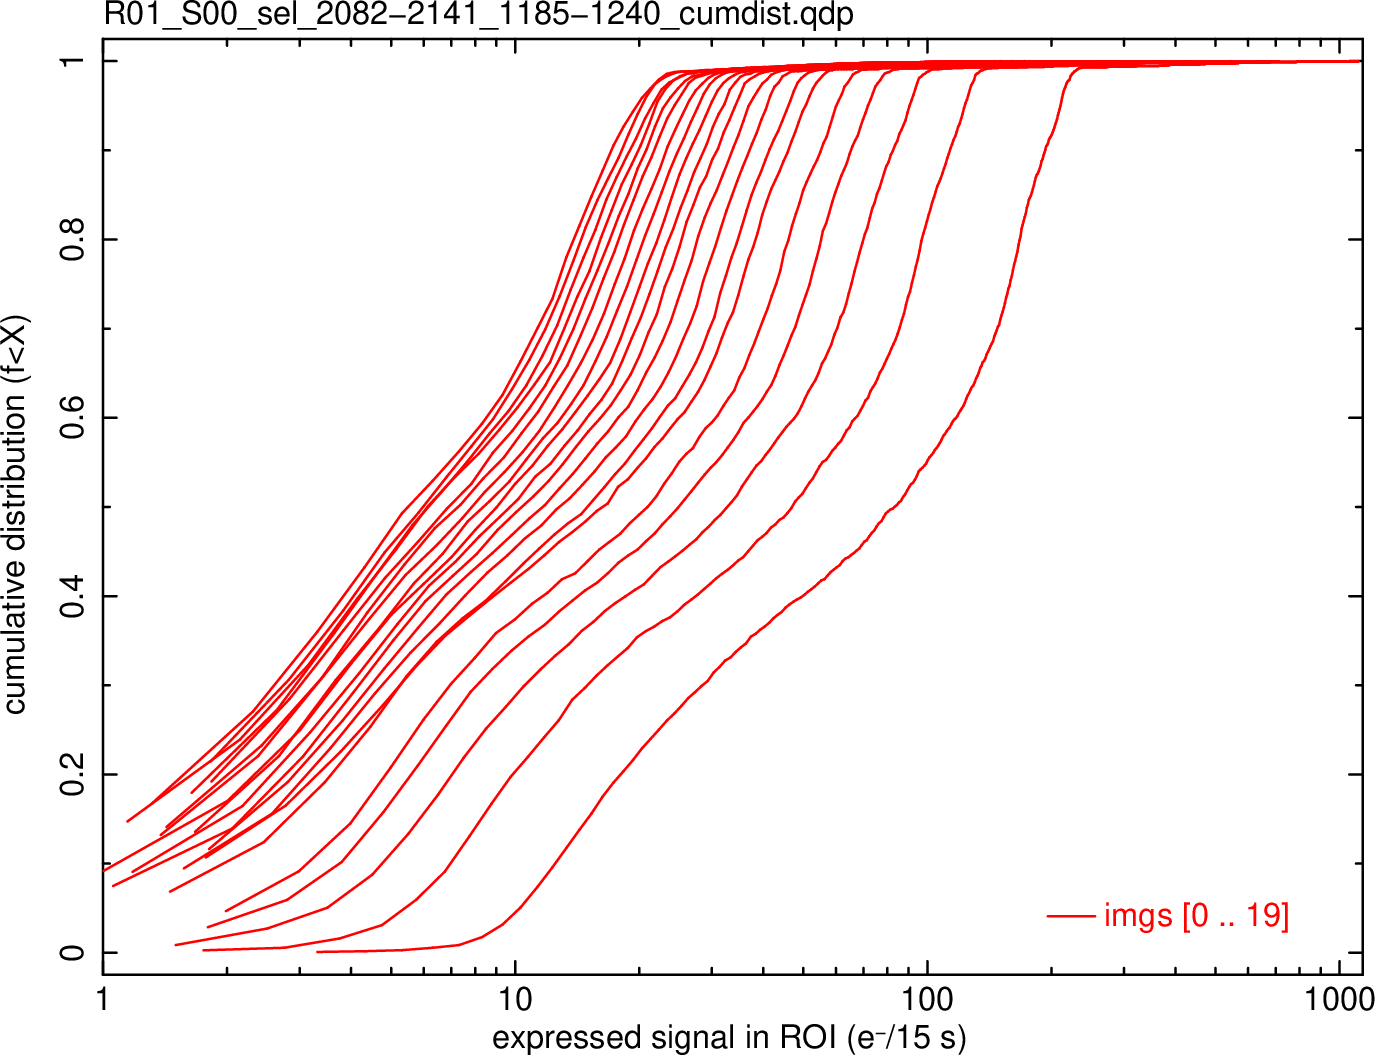
\includegraphics[width=\textwidth]{figures/phosphorescence-survey/phos_kinetics/R01_S00_sel_2082-2141_1185-1240_cumdist.png}    
\end{subfigure}
\hfil
\begin{subfigure}{0.45\textwidth}
  \centering
  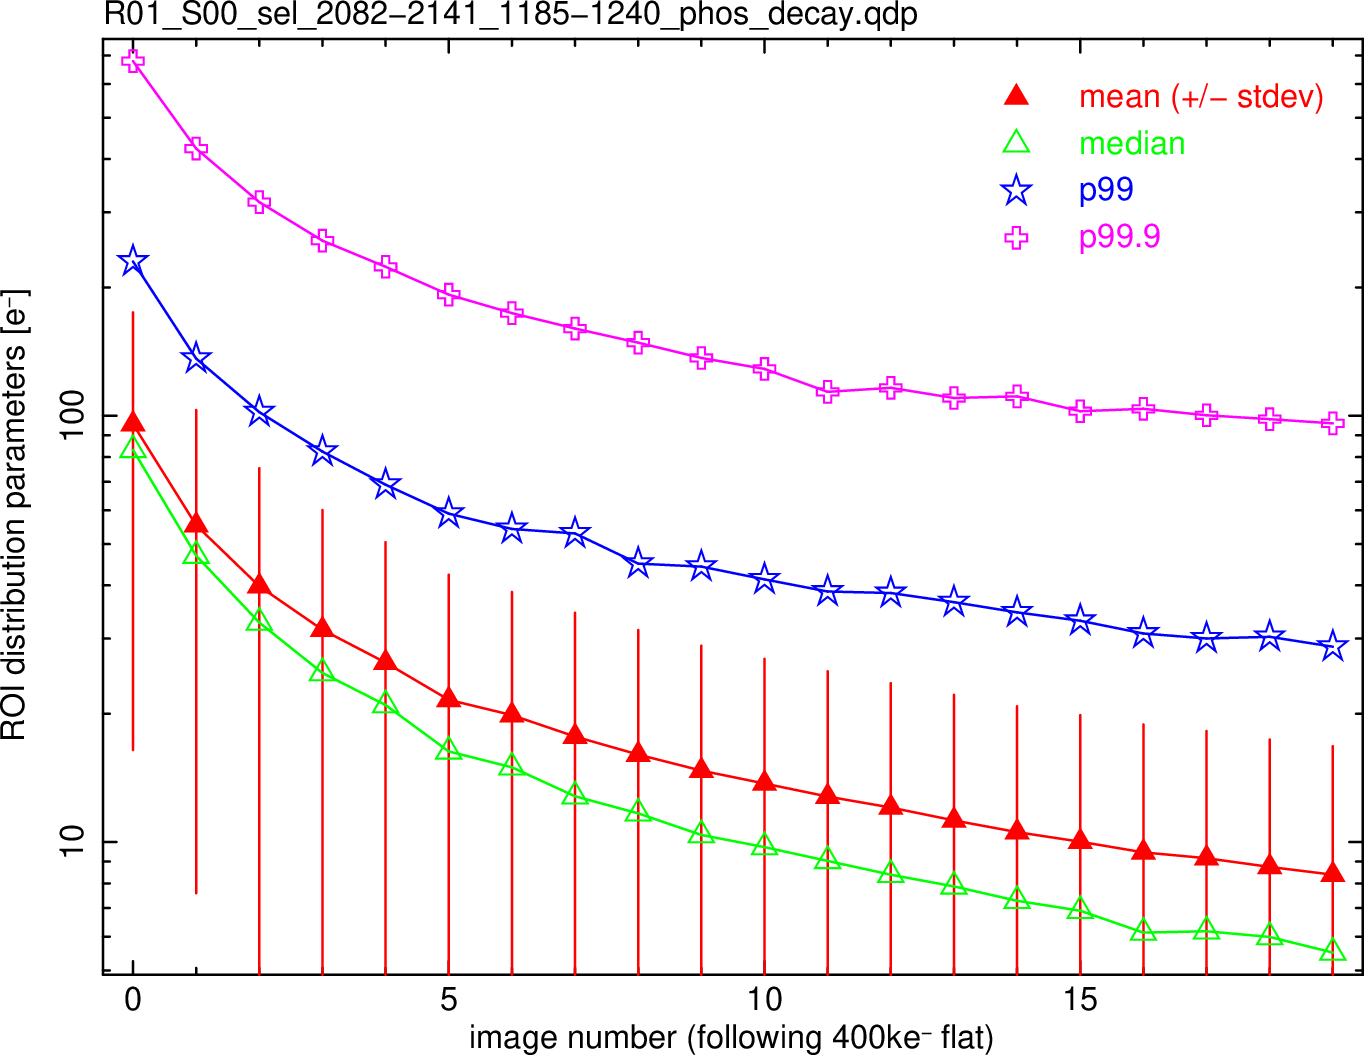
\includegraphics[width=\textwidth]{figures/phosphorescence-survey/phos_kinetics/R01_S00_sel_2082-2141_1185-1240_phos_decay.png}
\end{subfigure}
\newline
\caption{Kinetics for phosphorescence expression in ROIs of images for R01\_S00. This is the prominent cosmetic seen in Fig.~\ref{fig:phos:stains:R01S00}, which is apparently a {\it vampire} pixel.}
\label{fig:phos:kinetics:R01S00}
\end{figure}

\begin{figure}[!htbp]
\begin{subfigure}{0.45\textwidth}    
  \centering
  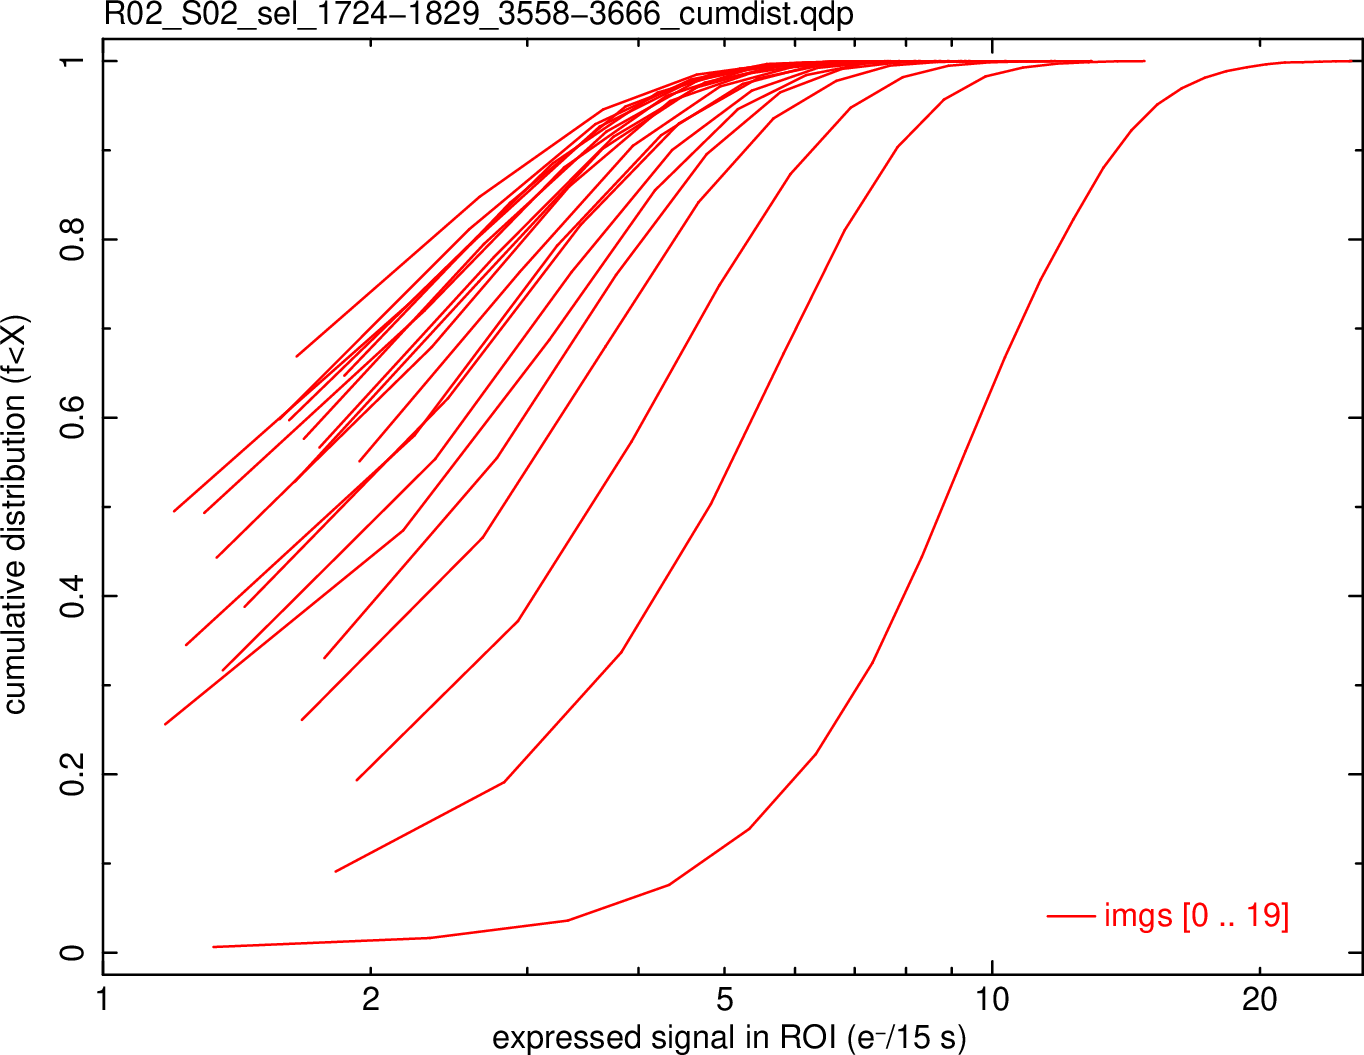
\includegraphics[width=\textwidth]{figures/phosphorescence-survey/phos_kinetics/R02_S02_sel_1724-1829_3558-3666_cumdist.png}    
\end{subfigure}
\hfil
\begin{subfigure}{0.45\textwidth}
  \centering
  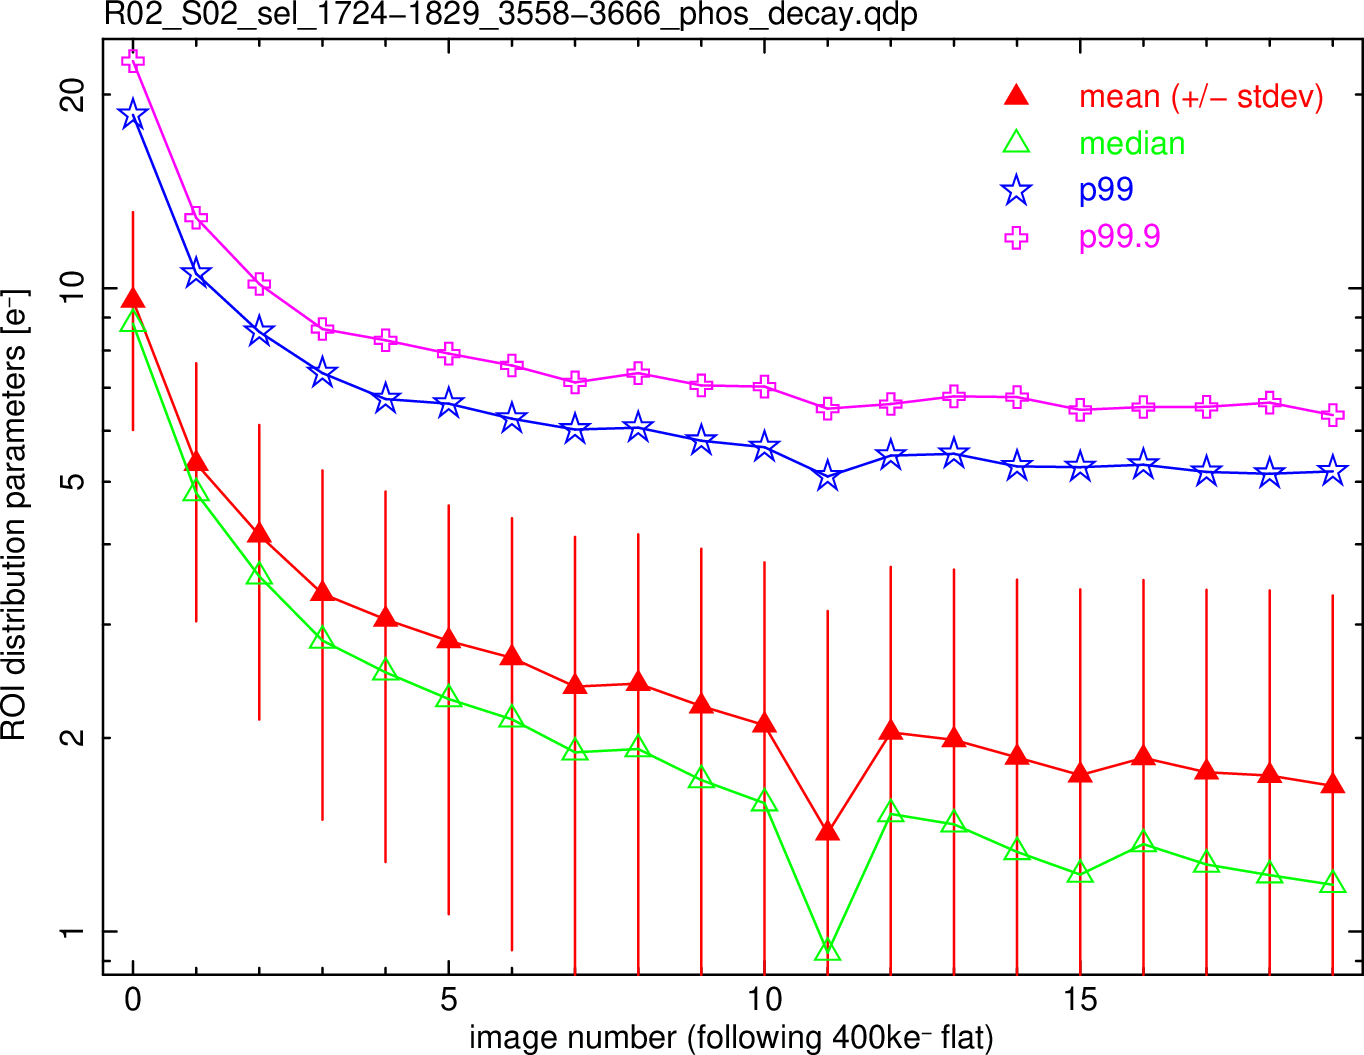
\includegraphics[width=\textwidth]{figures/phosphorescence-survey/phos_kinetics/R02_S02_sel_1724-1829_3558-3666_phos_decay.png}
\end{subfigure}
\newline
\begin{subfigure}{0.45\textwidth}    
  \centering
  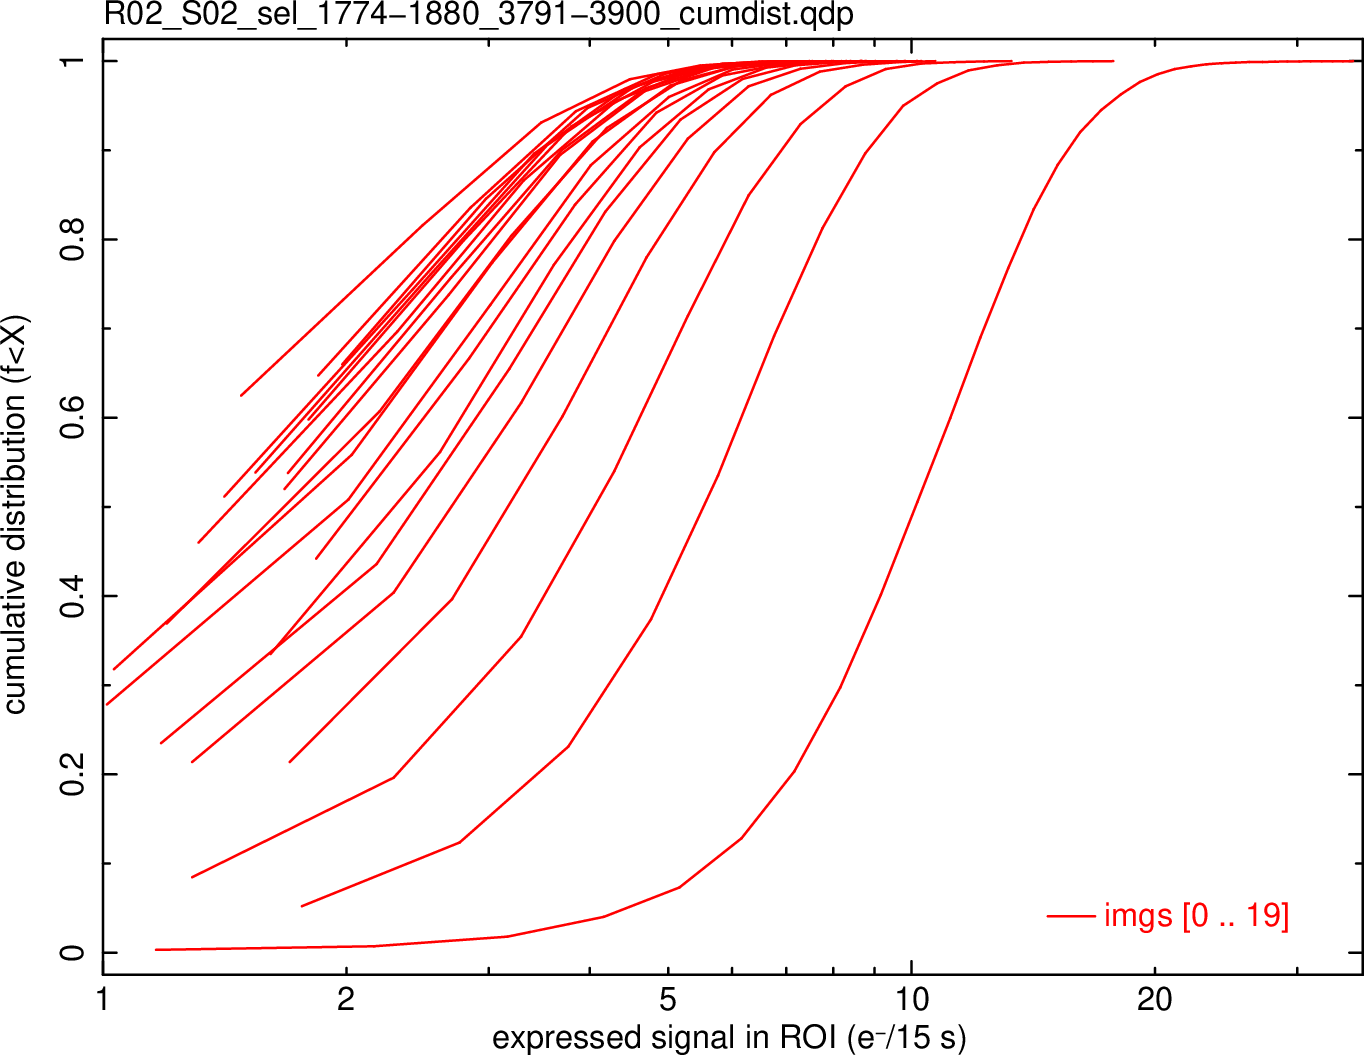
\includegraphics[width=\textwidth]{figures/phosphorescence-survey/phos_kinetics/R02_S02_sel_1774-1880_3791-3900_cumdist.png}    
\end{subfigure}
\hfil
\begin{subfigure}{0.45\textwidth}
  \centering
  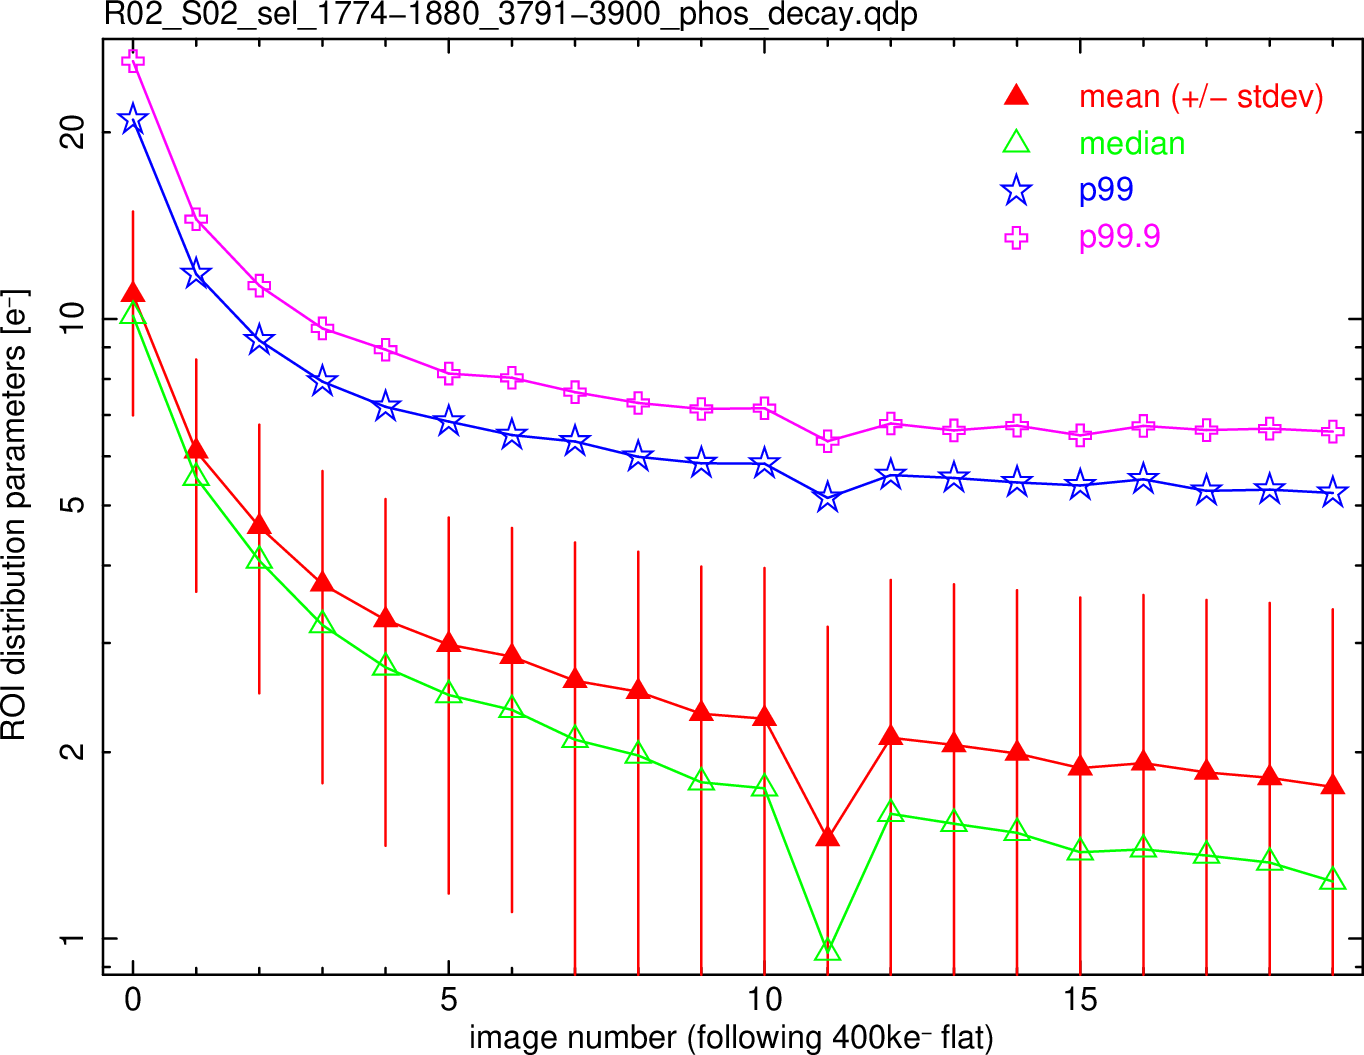
\includegraphics[width=\textwidth]{figures/phosphorescence-survey/phos_kinetics/R02_S02_sel_1774-1880_3791-3900_phos_decay.png}
\end{subfigure}
\newline
\begin{subfigure}{0.45\textwidth}    
  \centering
  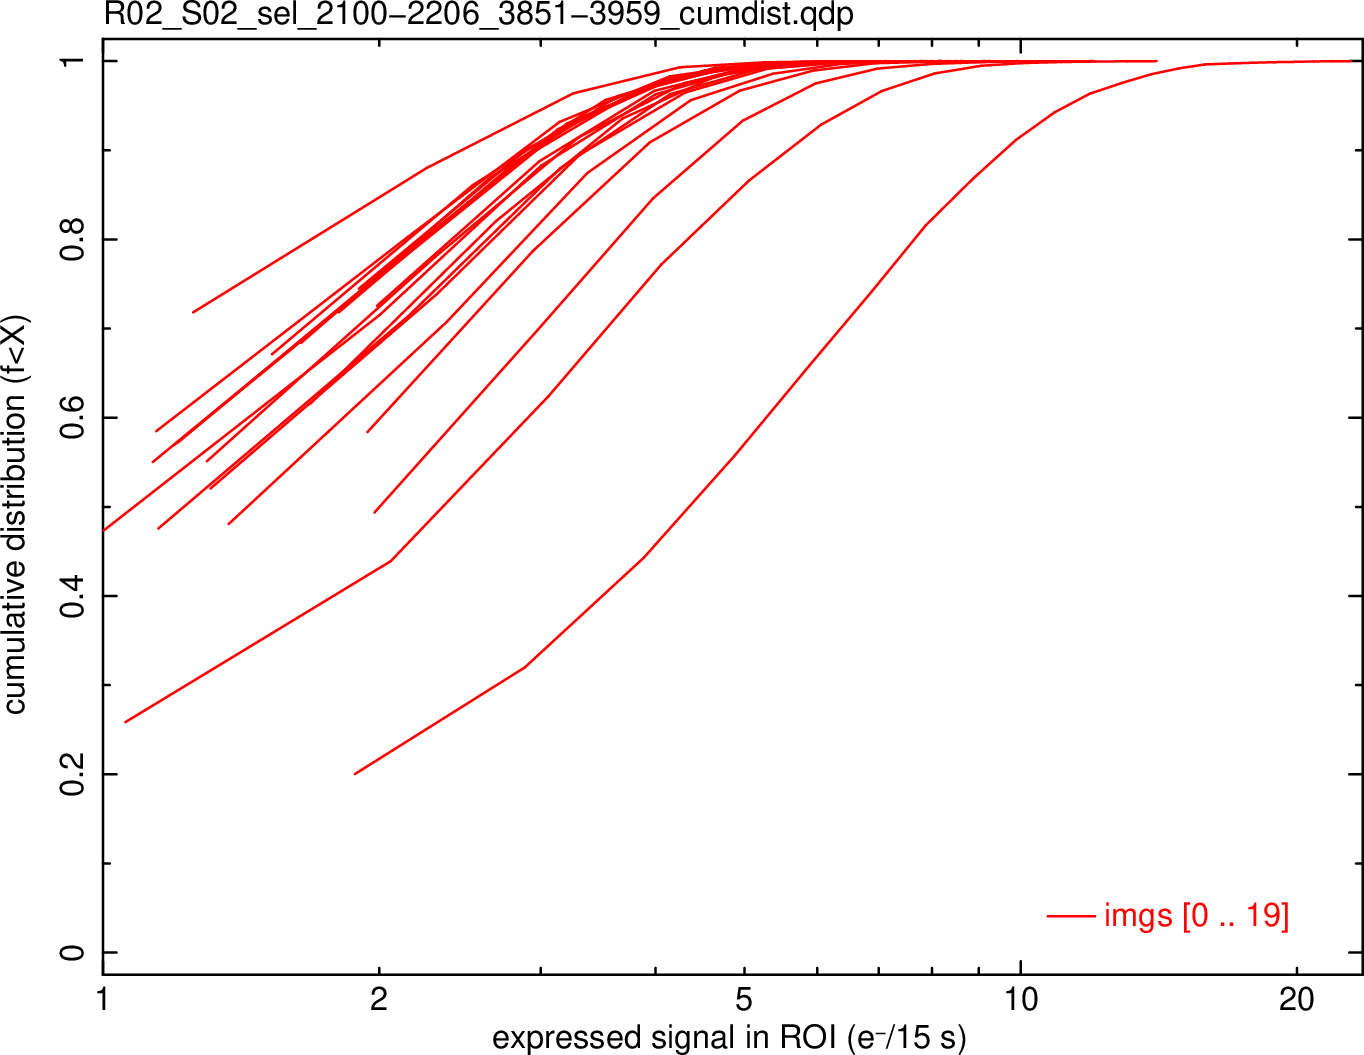
\includegraphics[width=\textwidth]{figures/phosphorescence-survey/phos_kinetics/R02_S02_sel_2100-2206_3851-3959_cumdist.png}    
\end{subfigure}
\hfil
\begin{subfigure}{0.45\textwidth}
  \centering
  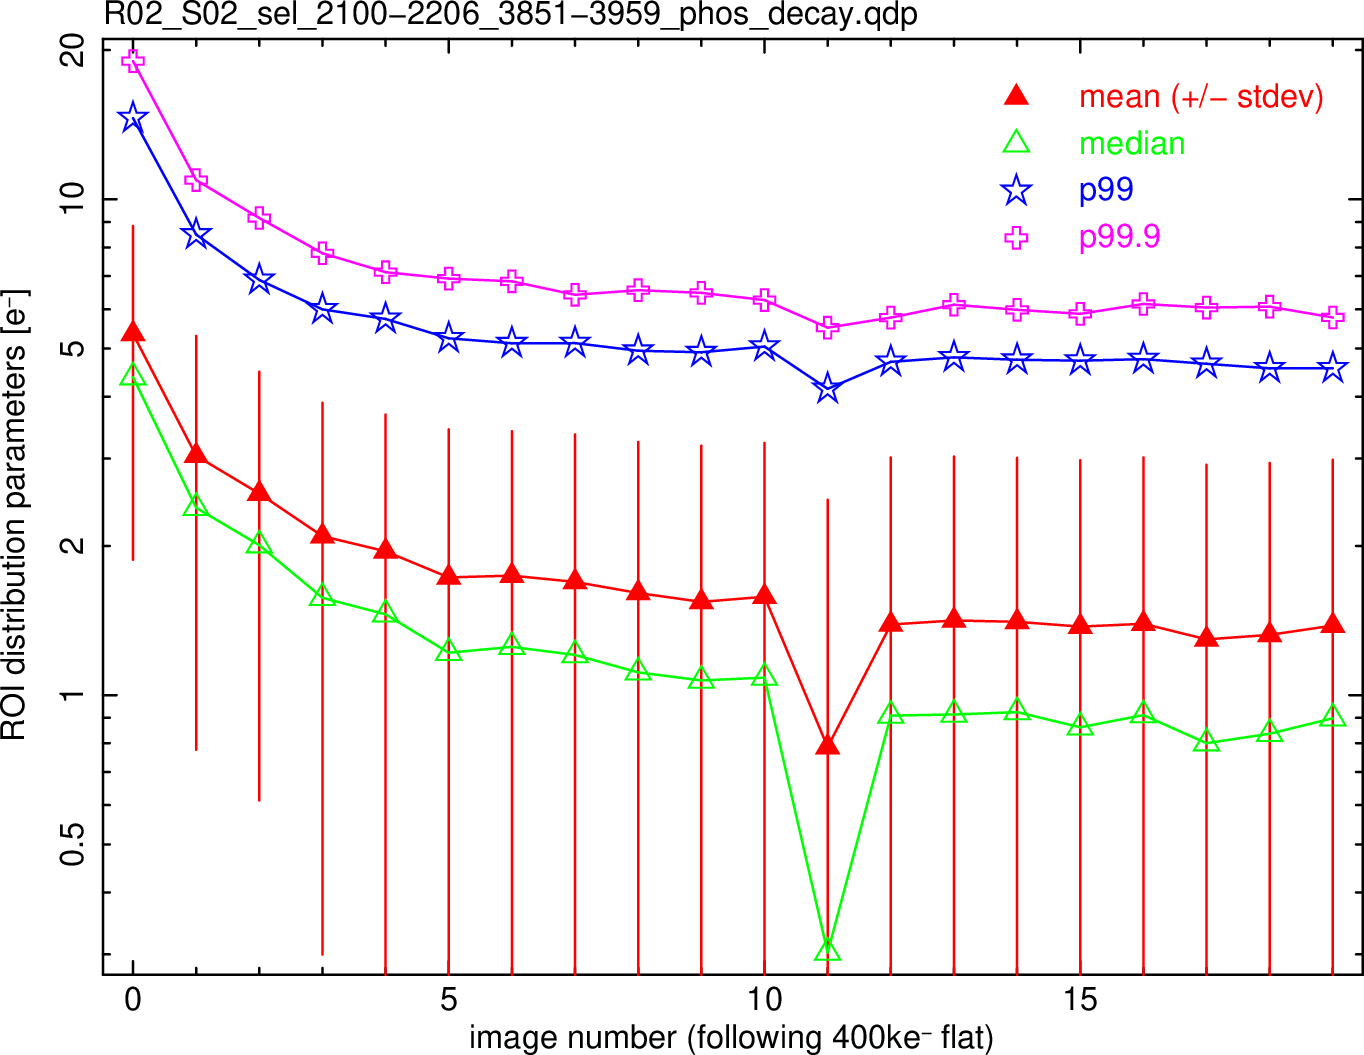
\includegraphics[width=\textwidth]{figures/phosphorescence-survey/phos_kinetics/R02_S02_sel_2100-2206_3851-3959_phos_decay.png}
\end{subfigure}
\newline
\caption{Kinetics for phosphorescence expression in ROIs of images for R02\_S02. This is the diffuse phosphorescence that correlates with the coffee stains seen in Fig.~\ref{fig:phos:stains:R02S02}. No extraction was performed on the {\it vampire pixel} found on the same sensor (R02\_S02\_C07).}
\label{fig:phos:kinetics:R02S02}
\end{figure}

\begin{figure}[!htbp]
\begin{subfigure}{0.45\textwidth}    
  \centering
  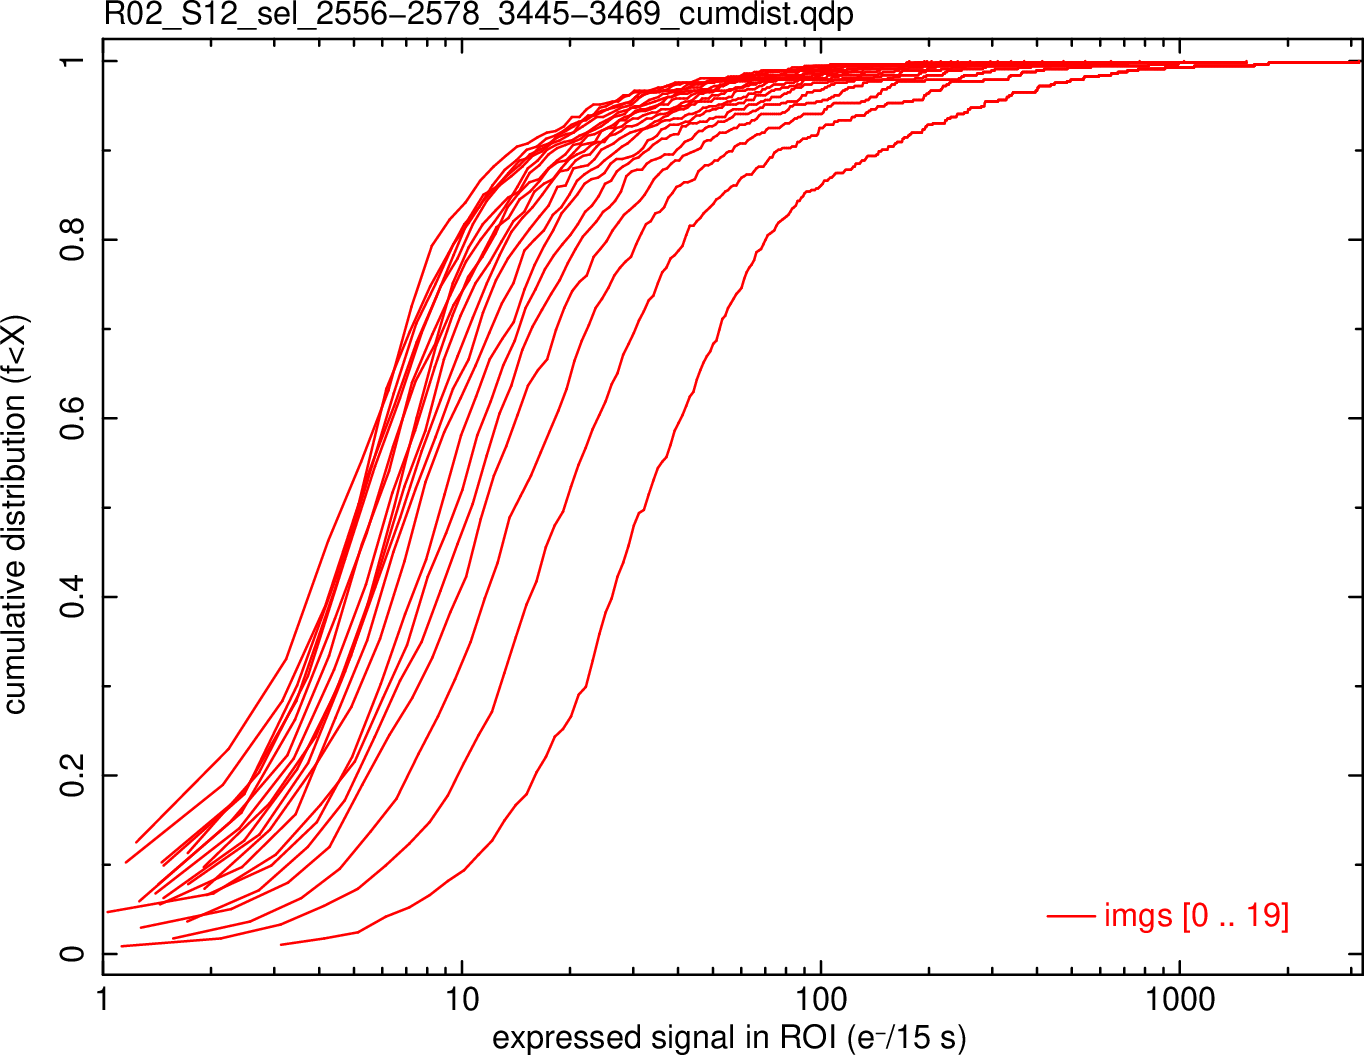
\includegraphics[width=\textwidth]{figures/phosphorescence-survey/phos_kinetics/R02_S12_sel_2556-2578_3445-3469_cumdist.png}    
\end{subfigure}
\hfil
\begin{subfigure}{0.45\textwidth}
  \centering
  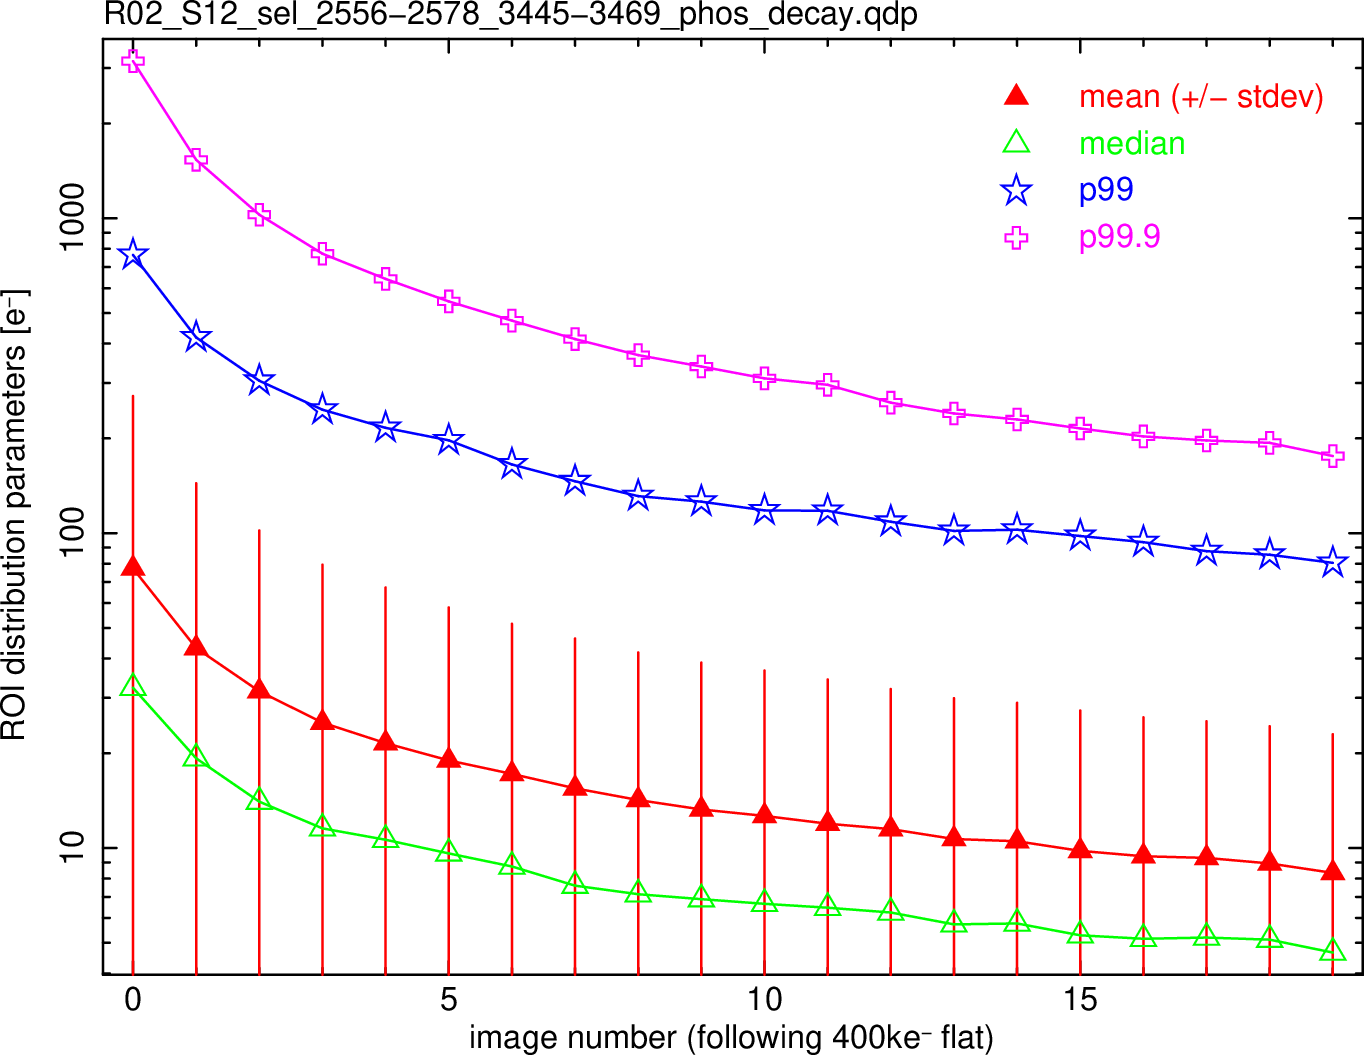
\includegraphics[width=\textwidth]{figures/phosphorescence-survey/phos_kinetics/R02_S12_sel_2556-2578_3445-3469_phos_decay.png}
\end{subfigure}
\newline
\begin{subfigure}{0.45\textwidth}    
  \centering
  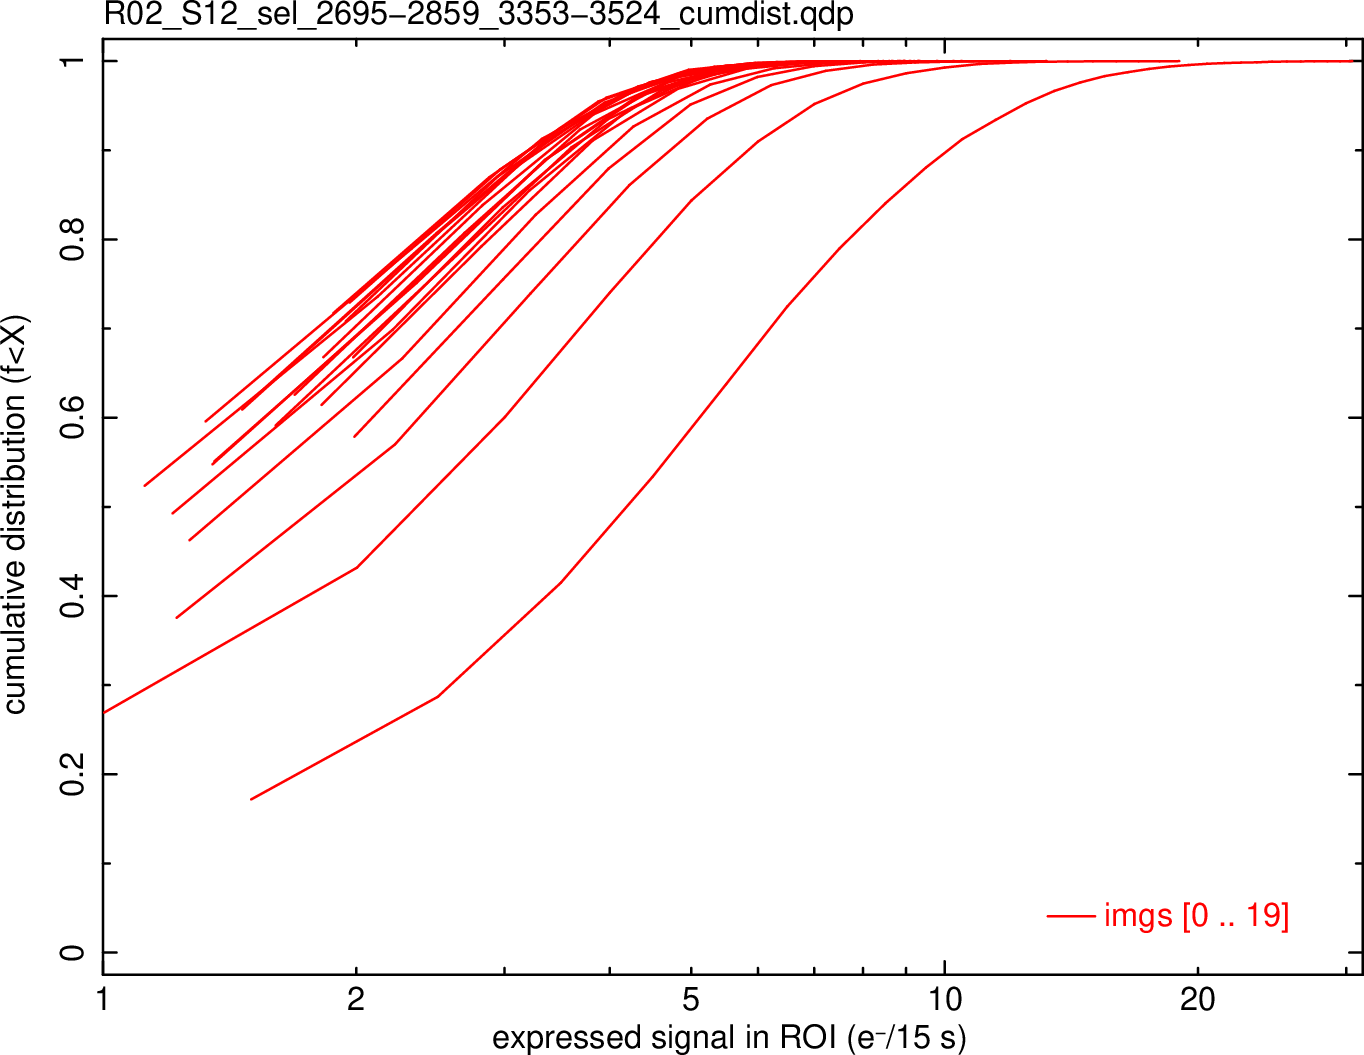
\includegraphics[width=\textwidth]{figures/phosphorescence-survey/phos_kinetics/R02_S12_sel_2695-2859_3353-3524_cumdist.png}    
\end{subfigure}
\hfil
\begin{subfigure}{0.45\textwidth}
  \centering
  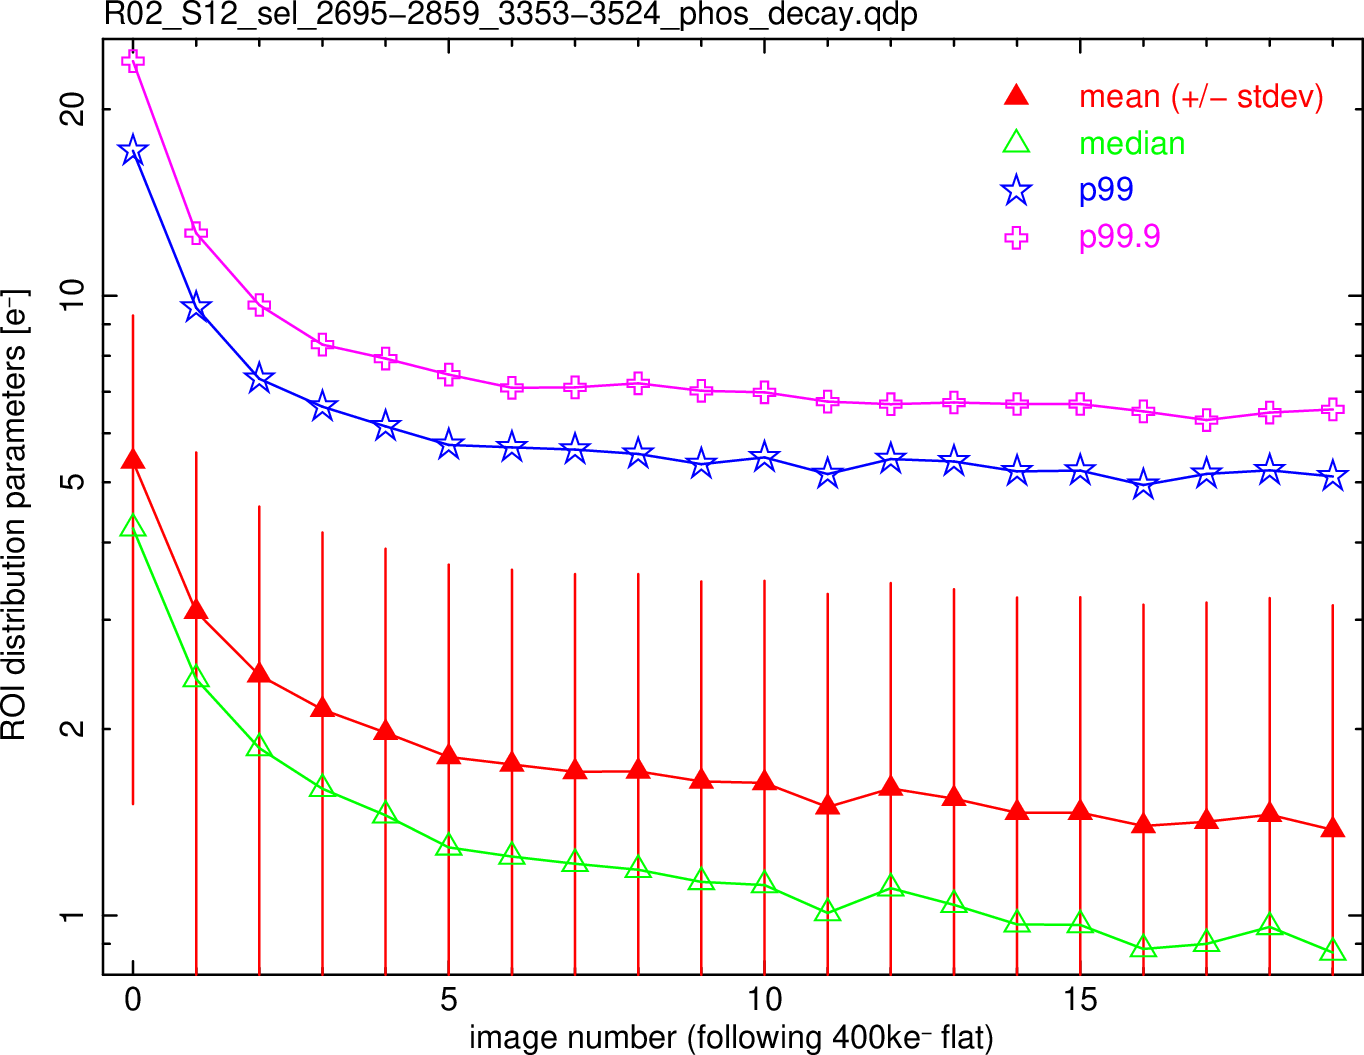
\includegraphics[width=\textwidth]{figures/phosphorescence-survey/phos_kinetics/R02_S12_sel_2695-2859_3353-3524_phos_decay.png}
\end{subfigure}
\newline
\begin{subfigure}{0.45\textwidth}    
  \centering
  \includegraphics[width=\textwidth]{figures/phosphorescence-survey/phos_kinetics/R02_S12_sel_523-676_9-129_cumdist.png}    
\end{subfigure}
\hfil
\begin{subfigure}{0.45\textwidth}
  \centering
  \includegraphics[width=\textwidth]{figures/phosphorescence-survey/phos_kinetics/R02_S12_sel_523-676_9-129_phos_decay.png}
\end{subfigure}
\newline
\caption{Kinetics for phosphorescence expression in ROIs of images for R02\_S12. This is the structured phosphorescence that correlates with the coffee stains seen in Fig.~\ref{fig:phos:stains:R02S12}.}
\label{fig:phos:kinetics:R02S12}
\end{figure}

\begin{figure}[!htbp]
\begin{subfigure}{0.45\textwidth}    
  \centering
  \includegraphics[width=\textwidth]{figures/phosphorescence-survey/phos_kinetics/R03_S10_sel_2969-3010_1763-1800_cumdist.png}    
\end{subfigure}
\hfil
\begin{subfigure}{0.45\textwidth}
  \centering
  \includegraphics[width=\textwidth]{figures/phosphorescence-survey/phos_kinetics/R03_S10_sel_2969-3010_1763-1800_phos_decay.png}
\end{subfigure}
\newline
\begin{subfigure}{0.45\textwidth}    
  \centering
  \includegraphics[width=\textwidth]{figures/phosphorescence-survey/phos_kinetics/R03_S10_sel_2970-2985_1767-1797_cumdist.png}    
\end{subfigure}
\hfil
\begin{subfigure}{0.45\textwidth}
  \centering
  \includegraphics[width=\textwidth]{figures/phosphorescence-survey/phos_kinetics/R03_S10_sel_2970-2985_1767-1797_phos_decay.png}
\end{subfigure}
\newline
\begin{subfigure}{0.45\textwidth}    
  \centering
  \includegraphics[width=\textwidth]{figures/phosphorescence-survey/phos_kinetics/R03_S10_sel_2995-3009_1767-1797_cumdist.png}    
\end{subfigure}
\hfil
\begin{subfigure}{0.45\textwidth}
  \centering
  \includegraphics[width=\textwidth]{figures/phosphorescence-survey/phos_kinetics/R03_S10_sel_2995-3009_1767-1797_phos_decay.png}
\end{subfigure}
\newline
\caption{Kinetics for phosphorescence expression in ROIs of images for R03\_S10. These describe regions including or near the bright/focusing {\it vampire pixel} seen in Figs.~\ref{fig:phos:stains:R03S10}, \ref{subfig:phosresp_R03_S10} and \ref{subfig:hvb_on_R03_S10}.}
\label{fig:phos:kinetics:R03S10}
\end{figure}

\begin{figure}[!htbp]
\begin{subfigure}{0.45\textwidth}    
  \centering
  \includegraphics[width=\textwidth]{figures/phosphorescence-survey/phos_kinetics/R20_S20_sel_1820-1920_535-635_cumdist.png}    
\end{subfigure}
\hfil
\begin{subfigure}{0.45\textwidth}
  \centering
  \includegraphics[width=\textwidth]{figures/phosphorescence-survey/phos_kinetics/R20_S20_sel_1820-1920_535-635_phos_decay.png}
\end{subfigure}
\newline
\caption{Kinetics for phosphorescence expression in ROIs of images for R20\_S20. These describe the prominent non-focusing {\it vampire pixel} seen in Figs.~\ref{subfig:phosresp_R20_S20} and \ref{subfig:hvb_on_R20_S20}.}
\label{fig:phos:kinetics:R20S20}
\end{figure}

\begin{figure}[!htbp]
\begin{subfigure}{0.45\textwidth}    
  \centering
  \includegraphics[width=\textwidth]{figures/phosphorescence-survey/phos_kinetics/R43_S11_sel_1741-1955_3754-3806_cumdist.png}    
\end{subfigure}
\hfil
\begin{subfigure}{0.45\textwidth}
  \centering
  \includegraphics[width=\textwidth]{figures/phosphorescence-survey/phos_kinetics/R43_S11_sel_1741-1955_3754-3806_phos_decay.png}
\end{subfigure}
\newline
\begin{subfigure}{0.45\textwidth}    
  \centering
  \includegraphics[width=\textwidth]{figures/phosphorescence-survey/phos_kinetics/R43_S11_sel_1763-1976_3826-3878_cumdist.png}    
\end{subfigure}
\hfil
\begin{subfigure}{0.45\textwidth}
  \centering
  \includegraphics[width=\textwidth]{figures/phosphorescence-survey/phos_kinetics/R43_S11_sel_1763-1976_3826-3878_phos_decay.png}
\end{subfigure}
\newline
\begin{subfigure}{0.45\textwidth}    
  \centering
  \includegraphics[width=\textwidth]{figures/phosphorescence-survey/phos_kinetics/R43_S11_sel_40-90_2751-2957_cumdist.png}    
\end{subfigure}
\hfil
\begin{subfigure}{0.45\textwidth}
  \centering
  \includegraphics[width=\textwidth]{figures/phosphorescence-survey/phos_kinetics/R43_S11_sel_40-90_2751-2957_phos_decay.png}
\end{subfigure}
\newline
\caption{Kinetics for phosphorescence expression in ROIs of images for R43\_S11. These describe bright, diffuse transient regions seen in Figs.~\ref{fig:phos:stains:R43S11} and \ref{subfig:hvb_on_R43_S11}, which apparently turn off completely when the HV Bias is {\it off}.}
\label{fig:phos:kinetics:R43S11}
\end{figure}

\begin{figure}[!htbp]
\begin{subfigure}{0.45\textwidth}    
  \centering
  \includegraphics[width=\textwidth]{figures/phosphorescence-survey/phos_kinetics/R43_S20_sel_207-292_3352-3435_cumdist.png}    
\end{subfigure}
\hfil
\begin{subfigure}{0.45\textwidth}
  \centering
  \includegraphics[width=\textwidth]{figures/phosphorescence-survey/phos_kinetics/R43_S20_sel_207-292_3352-3435_phos_decay.png}
\end{subfigure}
\newline
\begin{subfigure}{0.45\textwidth}    
  \centering
  \includegraphics[width=\textwidth]{figures/phosphorescence-survey/phos_kinetics/R43_S20_sel_547-633_3346-3430_cumdist.png}    
\end{subfigure}
\hfil
\begin{subfigure}{0.45\textwidth}
  \centering
  \includegraphics[width=\textwidth]{figures/phosphorescence-survey/phos_kinetics/R43_S20_sel_547-633_3346-3430_phos_decay.png}
\end{subfigure}
\newline
\begin{subfigure}{0.45\textwidth}    
  \centering
  \includegraphics[width=\textwidth]{figures/phosphorescence-survey/phos_kinetics/R43_S20_sel_707-816_3373-3589_cumdist.png}    
\end{subfigure}
\hfil
\begin{subfigure}{0.45\textwidth}
  \centering
  \includegraphics[width=\textwidth]{figures/phosphorescence-survey/phos_kinetics/R43_S20_sel_707-816_3373-3589_phos_decay.png}
\end{subfigure}
\newline
\caption{Kinetics for phosphorescence expression in ROIs of images for R43\_S20. These include some of the the highly structured {\it snowflake-like} transient regions seen in Figs.~\ref{subfig:hvb_on_R43_S20} and \ref{fig:phos:stains:R43S20}.}
\label{fig:phos:kinetics:R43S20}
\end{figure}

\clearpage
\section{Phosphorescence response characterization}
\label{sect:response}
Figures~\ref{fig:phos:resp:R01S00} through \ref{fig:phos:resp:R43S20} attempt to quantify the expressed phosphorescence response in ROIs on seven of the problematic ITL sensors. Previously, we had captured the phosphorescence {\it transient term} across the ITL sensors ({\it cf.} Figs.~\ref{fig:phos:R00} thru \ref{fig:phos:R44}); we also tracked ROI pixel distribution parameters of individual median images constructed from the selection of specific images acquired across the 20 B-protocol datasets available (listed in Table~\ref{tab:phosphorescence:datasets}). Here we analyze the signal level- and wavelength-dependences of the expressed phosphorescence captured in the first dark image following flat exposure. Table~XX provides the image numbers.. 

Because these runs were performed to sample a two dimensional parameter space,  that would lead to 

By fitting decay models to these persistence curves, it is immediately clear that there are multiple (>2) timescales at play for the pixels in each ROI. An example of such a fit is given in Figure~\ref{fig:phos:kinetics:fit:R20S20C13} where a 3-population relaxation model is used to characterize evolution of the 99\% quantile level of the distribution. In this case, there are three different exponential timescales determined: $(\tau_1,\tau_2,\tau_3) = (0.62,2.5,18.3)$ in image units (10.9, 43.8 \& 320 seconds, respectively). The corresponding ratio of these populations works out to 4.5\% (fast), 21.5\% (medium) and 74\% (slow), respectively. Inspection of the more detailed parameters plotted generally indicate skewed distributions from mismatches between medians and means; the choice of the 99\% quantile level to characterize was mainly to estimate the degree to which images would need to be phosphorescence-corrected (and/or the variance plane modified, given the asymmetric impact of the position specific, phosphorescence contribution in recorded images). 

%\begin{figure}[!htbp]
%\centering
%\begin{subfigure}{0.8\textwidth}    
%  \centering
%  \includegraphics[width=\textwidth]{figures/phosphorescence-%survey/phos_kinetics/R20_S20_sel_1820-1920_535-635_phos_decay_fit.png}    
%\end{subfigure}
%\caption{A three-population fit of the phosphorescence expressed by the %vapire pixel region of R20\_S20\_C13. The fit was performed on the 99\% %quantile level where signal levels are well above the $3\sigma$ level of %the noise distribution. Here, image numbers are parasitically used as %time units, with roughly 17.5 seconds per image.}
%\label{fig:phos:resp:fit:R20S20C13}
%\end{figure}

\begin{figure}[!htbp]
\centering
\begin{subfigure}{0.45\textwidth}    
  \centering
  \includegraphics[width=\textwidth]{figures/phosphorescence-survey/phos_resp/resp_99_R01_S00_1961-2020_1268-1325.png}    
\end{subfigure}
\newline
\centering
\begin{subfigure}{0.45\textwidth}    
  \centering
  \includegraphics[width=\textwidth]{figures/phosphorescence-survey/phos_resp/resp_99_R01_S00_1983-2042_1065-1121.png}    
\end{subfigure}
\newline
\centering
\begin{subfigure}{0.45\textwidth}    
  \centering
  \includegraphics[width=\textwidth]{figures/phosphorescence-survey/phos_resp/resp_99_R01_S00_2082-2141_1185-1240.png}    
\end{subfigure}
\newline
\caption{Signal and wavelength response for phosphorescence expression (99\% level) in ROIs of images for R01\_S00. This is the prominent cosmetic seen in Fig.~\ref{fig:phos:stains:R01S00}, which is apparently a {\it vampire} pixel.}
\label{fig:phos:resp:R01S00}
\end{figure}

\begin{figure}[!htbp]
\centering
\begin{subfigure}{0.45\textwidth}    
  \centering
  \includegraphics[width=\textwidth]{figures/phosphorescence-survey/phos_resp/resp_99_R02_S02_1724-1829_3558-3666.png}    
\end{subfigure}
\newline
\centering
\begin{subfigure}{0.45\textwidth}    
  \centering
  \includegraphics[width=\textwidth]{figures/phosphorescence-survey/phos_resp/resp_99_R02_S02_1774-1880_3791-3900.png}    
\end{subfigure}
\newline
\centering
\begin{subfigure}{0.45\textwidth}    
  \centering
  \includegraphics[width=\textwidth]{figures/phosphorescence-survey/phos_resp/resp_99_R02_S02_2100-2206_3851-3959.png}    
\end{subfigure}
\newline
\caption{Signal and wavelength response for phosphorescence expression (99\% level) in ROIs of images for R02\_S02. This is the diffuse phosphorescence that correlates with the coffee stains seen in Fig.~\ref{fig:phos:stains:R02S02}. No extractions were performed on the {\it vampire pixels} found on the same sensor (R02\_S02\_C15 and R02\_S02\_C07).}
\label{fig:phos:resp:R02S02}
\end{figure}

\begin{figure}[!htbp]
\centering
\begin{subfigure}{0.45\textwidth}    
  \centering
  \includegraphics[width=\textwidth]{figures/phosphorescence-survey/phos_resp/resp_99_R02_S12_2556-2578_3445-3469.png}    
\end{subfigure}
\newline
\centering
\begin{subfigure}{0.45\textwidth}    
  \centering
  \includegraphics[width=\textwidth]{figures/phosphorescence-survey/phos_resp/resp_99_R02_S12_2695-2859_3353-3524.png}    
\end{subfigure}
\newline
\centering
\begin{subfigure}{0.45\textwidth}    
  \centering
  \includegraphics[width=\textwidth]{figures/phosphorescence-survey/phos_resp/resp_99_R02_S12_523-676_9-129.png}    
\end{subfigure}
\newline
\caption{Signal and wavelength response for phosphorescence expression (99\% level) in ROIs of images for R02\_S12. This is the structured phosphorescence that correlates with the coffee stains seen in Fig.~\ref{fig:phos:stains:R02S12}.}
\label{fig:phos:resp:R02S12}
\end{figure}

\begin{figure}[!htbp]
\centering
\begin{subfigure}{0.45\textwidth}    
  \centering
  \includegraphics[width=\textwidth]{figures/phosphorescence-survey/phos_resp/resp_99_R03_S10_2969-3010_1763-1800.png}    
\end{subfigure}
\newline
\centering
\begin{subfigure}{0.45\textwidth}    
  \centering
  \includegraphics[width=\textwidth]{figures/phosphorescence-survey/phos_resp/resp_99_R03_S10_2970-2985_1767-1797.png}    
\end{subfigure}
\newline
\centering
\begin{subfigure}{0.45\textwidth}    
  \centering
  \includegraphics[width=\textwidth]{figures/phosphorescence-survey/phos_resp/resp_99_R03_S10_2995-3009_1767-1797.png}    
\end{subfigure}
\newline
\caption{Signal and wavelength response for phosphorescence expression (99\% level) in ROIs of images for R03\_S10. These describe regions including or near the bright/focusing {\it vampire pixel} seen in Figs.~\ref{fig:phos:stains:R03S10}, \ref{subfig:phosresp_R03_S10} and \ref{subfig:hvb_on_R03_S10}.}
\label{fig:phos:resp:R03S10}
\end{figure}

\begin{figure}[!htbp]
\centering
\begin{subfigure}{0.45\textwidth}    
  \centering
  \includegraphics[width=\textwidth]{figures/phosphorescence-survey/phos_resp/resp_99_R20_S20_1820-1920_535-635.png}    
\end{subfigure}
\newline
\caption{Signal and wavelength response for phosphorescence expression (99\% level) in an ROI of images for R20\_S20. These describe the prominent non-focusing {\it vampire pixel} seen in Figs.~\ref{subfig:phosresp_R20_S20} and \ref{subfig:hvb_on_R20_S20}.}
\label{fig:phos:kinetics:R20S20}
\end{figure}

\begin{figure}[!htbp]
\centering
\begin{subfigure}{0.45\textwidth}    
  \centering
  \includegraphics[width=\textwidth]{figures/phosphorescence-survey/phos_resp/resp_99_R43_S11_1741-1955_3754-3806.png}    
\end{subfigure}
\newline
\centering
\begin{subfigure}{0.45\textwidth}    
  \centering
  \includegraphics[width=\textwidth]{figures/phosphorescence-survey/phos_resp/resp_99_R43_S11_1763-1976_3826-3878.png}    
\end{subfigure}
\newline
\centering
\begin{subfigure}{0.45\textwidth}    
  \centering
  \includegraphics[width=\textwidth]{figures/phosphorescence-survey/phos_resp/resp_99_R43_S11_40-90_2751-2957.png}    
\end{subfigure}
\newline
\caption{Signal and wavelength response for phosphorescence expression (99\% level) in ROIs of images for R43\_S11. These describe bright, diffuse transient regions seen in Figs.~\ref{fig:phos:stains:R43S11} and \ref{subfig:hvb_on_R43_S11}, which apparently turn off completely when the HV Bias is {\it off}.}
\label{fig:phos:resp:R43S11}
\end{figure}

\begin{figure}[!htbp]
\centering
\begin{subfigure}{0.45\textwidth}    
  \centering
  \includegraphics[width=\textwidth]{figures/phosphorescence-survey/phos_resp/resp_99_R43_S20_207-292_3352-3435.png}    
\end{subfigure}
\newline
\centering
\begin{subfigure}{0.45\textwidth}    
  \centering
  \includegraphics[width=\textwidth]{figures/phosphorescence-survey/phos_resp/resp_99_R43_S20_547-633_3346-3430.png}    
\end{subfigure}
\newline
\centering
\begin{subfigure}{0.45\textwidth}    
  \centering
  \includegraphics[width=\textwidth]{figures/phosphorescence-survey/phos_resp/resp_99_R43_S20_707-816_3373-3589.png}    
\end{subfigure}
\newline
\caption{Signal and wavelength response for phosphorescence expression (99\% level) in ROIs of images for R43\_S20. These include some of the the highly structured {\it snowflake-like} transient regions seen in Figs.~\ref{subfig:hvb_on_R43_S20} and \ref{fig:phos:stains:R43S20}.}
\label{fig:phos:resp:R43S20}
\end{figure}

\clearpage
